% Options for packages loaded elsewhere
\PassOptionsToPackage{unicode}{hyperref}
\PassOptionsToPackage{hyphens}{url}
\PassOptionsToPackage{dvipsnames,svgnames,x11names}{xcolor}
%
\documentclass[
  letterpaper,
  DIV=11,
  numbers=noendperiod]{scrreprt}

\usepackage{amsmath,amssymb}
\usepackage{lmodern}
\usepackage{iftex}
\ifPDFTeX
  \usepackage[T1]{fontenc}
  \usepackage[utf8]{inputenc}
  \usepackage{textcomp} % provide euro and other symbols
\else % if luatex or xetex
  \usepackage{unicode-math}
  \defaultfontfeatures{Scale=MatchLowercase}
  \defaultfontfeatures[\rmfamily]{Ligatures=TeX,Scale=1}
\fi
% Use upquote if available, for straight quotes in verbatim environments
\IfFileExists{upquote.sty}{\usepackage{upquote}}{}
\IfFileExists{microtype.sty}{% use microtype if available
  \usepackage[]{microtype}
  \UseMicrotypeSet[protrusion]{basicmath} % disable protrusion for tt fonts
}{}
\makeatletter
\@ifundefined{KOMAClassName}{% if non-KOMA class
  \IfFileExists{parskip.sty}{%
    \usepackage{parskip}
  }{% else
    \setlength{\parindent}{0pt}
    \setlength{\parskip}{6pt plus 2pt minus 1pt}}
}{% if KOMA class
  \KOMAoptions{parskip=half}}
\makeatother
\usepackage{xcolor}
\setlength{\emergencystretch}{3em} % prevent overfull lines
\setcounter{secnumdepth}{5}
% Make \paragraph and \subparagraph free-standing
\ifx\paragraph\undefined\else
  \let\oldparagraph\paragraph
  \renewcommand{\paragraph}[1]{\oldparagraph{#1}\mbox{}}
\fi
\ifx\subparagraph\undefined\else
  \let\oldsubparagraph\subparagraph
  \renewcommand{\subparagraph}[1]{\oldsubparagraph{#1}\mbox{}}
\fi

\usepackage{color}
\usepackage{fancyvrb}
\newcommand{\VerbBar}{|}
\newcommand{\VERB}{\Verb[commandchars=\\\{\}]}
\DefineVerbatimEnvironment{Highlighting}{Verbatim}{commandchars=\\\{\}}
% Add ',fontsize=\small' for more characters per line
\usepackage{framed}
\definecolor{shadecolor}{RGB}{241,243,245}
\newenvironment{Shaded}{\begin{snugshade}}{\end{snugshade}}
\newcommand{\AlertTok}[1]{\textcolor[rgb]{0.68,0.00,0.00}{#1}}
\newcommand{\AnnotationTok}[1]{\textcolor[rgb]{0.37,0.37,0.37}{#1}}
\newcommand{\AttributeTok}[1]{\textcolor[rgb]{0.40,0.45,0.13}{#1}}
\newcommand{\BaseNTok}[1]{\textcolor[rgb]{0.68,0.00,0.00}{#1}}
\newcommand{\BuiltInTok}[1]{\textcolor[rgb]{0.00,0.23,0.31}{#1}}
\newcommand{\CharTok}[1]{\textcolor[rgb]{0.13,0.47,0.30}{#1}}
\newcommand{\CommentTok}[1]{\textcolor[rgb]{0.37,0.37,0.37}{#1}}
\newcommand{\CommentVarTok}[1]{\textcolor[rgb]{0.37,0.37,0.37}{\textit{#1}}}
\newcommand{\ConstantTok}[1]{\textcolor[rgb]{0.56,0.35,0.01}{#1}}
\newcommand{\ControlFlowTok}[1]{\textcolor[rgb]{0.00,0.23,0.31}{#1}}
\newcommand{\DataTypeTok}[1]{\textcolor[rgb]{0.68,0.00,0.00}{#1}}
\newcommand{\DecValTok}[1]{\textcolor[rgb]{0.68,0.00,0.00}{#1}}
\newcommand{\DocumentationTok}[1]{\textcolor[rgb]{0.37,0.37,0.37}{\textit{#1}}}
\newcommand{\ErrorTok}[1]{\textcolor[rgb]{0.68,0.00,0.00}{#1}}
\newcommand{\ExtensionTok}[1]{\textcolor[rgb]{0.00,0.23,0.31}{#1}}
\newcommand{\FloatTok}[1]{\textcolor[rgb]{0.68,0.00,0.00}{#1}}
\newcommand{\FunctionTok}[1]{\textcolor[rgb]{0.28,0.35,0.67}{#1}}
\newcommand{\ImportTok}[1]{\textcolor[rgb]{0.00,0.46,0.62}{#1}}
\newcommand{\InformationTok}[1]{\textcolor[rgb]{0.37,0.37,0.37}{#1}}
\newcommand{\KeywordTok}[1]{\textcolor[rgb]{0.00,0.23,0.31}{#1}}
\newcommand{\NormalTok}[1]{\textcolor[rgb]{0.00,0.23,0.31}{#1}}
\newcommand{\OperatorTok}[1]{\textcolor[rgb]{0.37,0.37,0.37}{#1}}
\newcommand{\OtherTok}[1]{\textcolor[rgb]{0.00,0.23,0.31}{#1}}
\newcommand{\PreprocessorTok}[1]{\textcolor[rgb]{0.68,0.00,0.00}{#1}}
\newcommand{\RegionMarkerTok}[1]{\textcolor[rgb]{0.00,0.23,0.31}{#1}}
\newcommand{\SpecialCharTok}[1]{\textcolor[rgb]{0.37,0.37,0.37}{#1}}
\newcommand{\SpecialStringTok}[1]{\textcolor[rgb]{0.13,0.47,0.30}{#1}}
\newcommand{\StringTok}[1]{\textcolor[rgb]{0.13,0.47,0.30}{#1}}
\newcommand{\VariableTok}[1]{\textcolor[rgb]{0.07,0.07,0.07}{#1}}
\newcommand{\VerbatimStringTok}[1]{\textcolor[rgb]{0.13,0.47,0.30}{#1}}
\newcommand{\WarningTok}[1]{\textcolor[rgb]{0.37,0.37,0.37}{\textit{#1}}}

\providecommand{\tightlist}{%
  \setlength{\itemsep}{0pt}\setlength{\parskip}{0pt}}\usepackage{longtable,booktabs,array}
\usepackage{calc} % for calculating minipage widths
% Correct order of tables after \paragraph or \subparagraph
\usepackage{etoolbox}
\makeatletter
\patchcmd\longtable{\par}{\if@noskipsec\mbox{}\fi\par}{}{}
\makeatother
% Allow footnotes in longtable head/foot
\IfFileExists{footnotehyper.sty}{\usepackage{footnotehyper}}{\usepackage{footnote}}
\makesavenoteenv{longtable}
\usepackage{graphicx}
\makeatletter
\def\maxwidth{\ifdim\Gin@nat@width>\linewidth\linewidth\else\Gin@nat@width\fi}
\def\maxheight{\ifdim\Gin@nat@height>\textheight\textheight\else\Gin@nat@height\fi}
\makeatother
% Scale images if necessary, so that they will not overflow the page
% margins by default, and it is still possible to overwrite the defaults
% using explicit options in \includegraphics[width, height, ...]{}
\setkeys{Gin}{width=\maxwidth,height=\maxheight,keepaspectratio}
% Set default figure placement to htbp
\makeatletter
\def\fps@figure{htbp}
\makeatother
\newlength{\cslhangindent}
\setlength{\cslhangindent}{1.5em}
\newlength{\csllabelwidth}
\setlength{\csllabelwidth}{3em}
\newlength{\cslentryspacingunit} % times entry-spacing
\setlength{\cslentryspacingunit}{\parskip}
\newenvironment{CSLReferences}[2] % #1 hanging-ident, #2 entry spacing
 {% don't indent paragraphs
  \setlength{\parindent}{0pt}
  % turn on hanging indent if param 1 is 1
  \ifodd #1
  \let\oldpar\par
  \def\par{\hangindent=\cslhangindent\oldpar}
  \fi
  % set entry spacing
  \setlength{\parskip}{#2\cslentryspacingunit}
 }%
 {}
\usepackage{calc}
\newcommand{\CSLBlock}[1]{#1\hfill\break}
\newcommand{\CSLLeftMargin}[1]{\parbox[t]{\csllabelwidth}{#1}}
\newcommand{\CSLRightInline}[1]{\parbox[t]{\linewidth - \csllabelwidth}{#1}\break}
\newcommand{\CSLIndent}[1]{\hspace{\cslhangindent}#1}

\usepackage{booktabs}
\usepackage{caption}
\usepackage{longtable}
\usepackage{colortbl}
\usepackage{array}
\usepackage{anyfontsize}
\usepackage{multirow}
\KOMAoption{captions}{tableheading}
\makeatletter
\makeatother
\makeatletter
\@ifpackageloaded{bookmark}{}{\usepackage{bookmark}}
\makeatother
\makeatletter
\@ifpackageloaded{caption}{}{\usepackage{caption}}
\AtBeginDocument{%
\ifdefined\contentsname
  \renewcommand*\contentsname{Table of contents}
\else
  \newcommand\contentsname{Table of contents}
\fi
\ifdefined\listfigurename
  \renewcommand*\listfigurename{List of Figures}
\else
  \newcommand\listfigurename{List of Figures}
\fi
\ifdefined\listtablename
  \renewcommand*\listtablename{List of Tables}
\else
  \newcommand\listtablename{List of Tables}
\fi
\ifdefined\figurename
  \renewcommand*\figurename{Figure}
\else
  \newcommand\figurename{Figure}
\fi
\ifdefined\tablename
  \renewcommand*\tablename{Table}
\else
  \newcommand\tablename{Table}
\fi
}
\@ifpackageloaded{float}{}{\usepackage{float}}
\floatstyle{ruled}
\@ifundefined{c@chapter}{\newfloat{codelisting}{h}{lop}}{\newfloat{codelisting}{h}{lop}[chapter]}
\floatname{codelisting}{Listing}
\newcommand*\listoflistings{\listof{codelisting}{List of Listings}}
\makeatother
\makeatletter
\@ifpackageloaded{caption}{}{\usepackage{caption}}
\@ifpackageloaded{subcaption}{}{\usepackage{subcaption}}
\makeatother
\makeatletter
\@ifpackageloaded{tcolorbox}{}{\usepackage[many]{tcolorbox}}
\makeatother
\makeatletter
\@ifundefined{shadecolor}{\definecolor{shadecolor}{rgb}{.97, .97, .97}}
\makeatother
\makeatletter
\makeatother
\ifLuaTeX
  \usepackage{selnolig}  % disable illegal ligatures
\fi
\IfFileExists{bookmark.sty}{\usepackage{bookmark}}{\usepackage{hyperref}}
\IfFileExists{xurl.sty}{\usepackage{xurl}}{} % add URL line breaks if available
\urlstyle{same} % disable monospaced font for URLs
\hypersetup{
  pdftitle={Apuntes Prácticas de la asignatura de Bioestadística},
  pdfauthor={Jesús Esteban Hernández y Jesús Martín Fernández},
  colorlinks=true,
  linkcolor={blue},
  filecolor={Maroon},
  citecolor={Blue},
  urlcolor={Blue},
  pdfcreator={LaTeX via pandoc}}

\title{Apuntes Prácticas de la asignatura de Bioestadística}
\usepackage{etoolbox}
\makeatletter
\providecommand{\subtitle}[1]{% add subtitle to \maketitle
  \apptocmd{\@title}{\par {\large #1 \par}}{}{}
}
\makeatother
\subtitle{Grado de Medicina - URJC. Primer curso}
\author{Jesús Esteban Hernández y Jesús Martín Fernández}
\date{4/9/25}

\begin{document}
\maketitle
\ifdefined\Shaded\renewenvironment{Shaded}{\begin{tcolorbox}[enhanced, interior hidden, boxrule=0pt, borderline west={3pt}{0pt}{shadecolor}, frame hidden, breakable, sharp corners]}{\end{tcolorbox}}\fi

\renewcommand*\contentsname{Table of contents}
{
\hypersetup{linkcolor=}
\setcounter{tocdepth}{2}
\tableofcontents
}
\bookmarksetup{startatroot}

\hypertarget{preface}{%
\chapter*{Preface}\label{preface}}
\addcontentsline{toc}{chapter}{Preface}

\markboth{Preface}{Preface}

This is a Quarto book.

To learn more about Quarto books visit
\url{https://quarto.org/docs/books}.

\begin{Shaded}
\begin{Highlighting}[]
\DecValTok{1} \SpecialCharTok{+} \DecValTok{1}
\end{Highlighting}
\end{Shaded}

\begin{verbatim}
[1] 2
\end{verbatim}

\bookmarksetup{startatroot}

\hypertarget{pr0-buenas-pruxe1cticas-en-recopilaciuxf3n-de-datos}{%
\chapter{PR0-Buenas prácticas en recopilación de
datos}\label{pr0-buenas-pruxe1cticas-en-recopilaciuxf3n-de-datos}}

Antes de comenzar\ldots{}

La crisis de la reproducibilidad..

Aunque con frecuencia se utilizan como sinónimos, en investigación
\textbf{reproducibilidad} y \textbf{replicabilidad} no significan lo
mismo.

\begin{quote}
Un estudio de investigación es \textbf{reproducible} si al repetir el
análisis utilizando los mismos métodos de investigación (no solo el
mismo análisis estadístico, pero también dicho análisis) \textbf{sobre
los mismos datos} obtenemos los mismos resultados. Indica que el estudio
fue realizado conforme se indica, incluyendo el análisis.
\end{quote}

\begin{quote}
Un estudio de investigación es \textbf{replicable} si repitiendo el
proceso de investigación con la misma metodología, pero \textbf{sobre
nuevos datos} obtenemos los mismos resultados, lo que indica que podemos
confiar en sus conclusiones. Las razones para la falta de replicabilidad
no son solo achacables
\end{quote}

\begin{itemize}
\tightlist
\item
  \textbf{Reproducibilidad (reproducibility)} y \textbf{replicabilidad
  (replicability)} condicionan la \textbf{fiabilidad (reliability)} de
  nuestros hallazgos.
\item
  La \textbf{reproducibilidad} es condición necesaria pero no suficiente
  para la \textbf{replicabilidad}.
\end{itemize}

\begin{figure}

{\centering 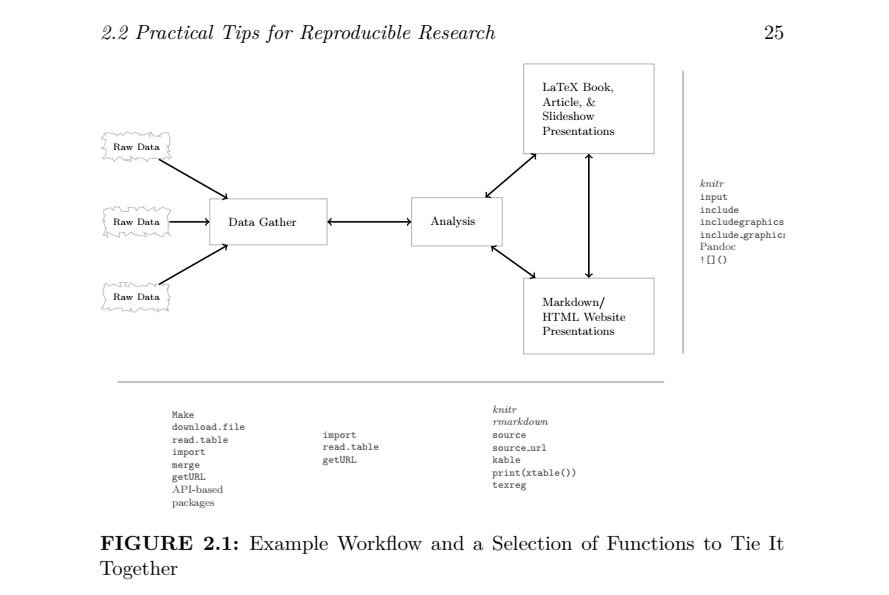
\includegraphics{./pics/tips_repro_res_gandrupbook.png}

}

\caption{Imagen tomada de Gandrud (2020)}

\end{figure}

Este documento no aborda aspectos como la instalación de R y RStudio,
aspectos bien cubiertos en muchos otros recursos, algunos mencionados en
la bibliografía.

El siguiente esquema trata de representar el flujo de trabajo habitual
en cualquier proyecto de data science independientemente de su
envergadura.

En la preparación de cualquier trabajo de investigación en el que
nosotros nos encarguemos del análisis pasaremos por todas o casi todas
estas fases.

En sentido estricto, el análisis estadístico sería el ciclo
Transform-Visualise-Model, pero es imposible llegar a estas fases si no
se completan los pasos anteriores. De igual manera, sería extraño
realizar un análisis para no comunicarlo, por lo que, aunque las
siguientes notas no siguen exactamente este esquema, es importante
tratar de pensar a qué fase corresponde todo lo que veremos en los
seminarios prácticos, por lo que con frecuencia recurriremos a este
esquema.

\begin{figure}

{\centering 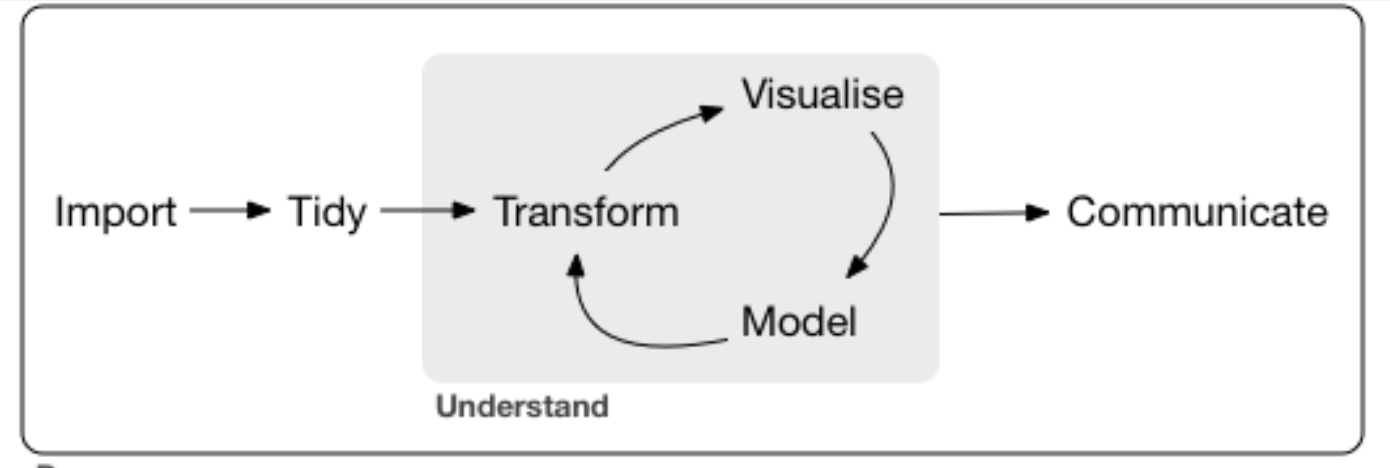
\includegraphics{./pics/datascience_proj.png}

}

\caption{Data Science WorkFlow}

\end{figure}

Como veremos al termina la sección, no siempre contamos con la mejor
solución a la hora de recoger los datos, pero esto no evita la necesidad
de recogerlos con la mayor calidad posible, tarea que comienza incluso
antes de su recogida. Siendo esencial, en esta sesión no hablaremos de
la importancia de la definición adecuada de las variables, algunos de
cuyos aspectos habrán sido ya comentados en las clases presenciales. En
este texto solo daremos algunas pautas para mejorar su introducción en
el primero soporte disponible antes a su importación al software de
análisis.

\hypertarget{buenas-pruxe1cticas-sobre-gestiuxf3n-de-datos.}{%
\section{Buenas prácticas sobre gestión de
datos.}\label{buenas-pruxe1cticas-sobre-gestiuxf3n-de-datos.}}

Poco textos sobre estadística incluyen un apartado sobre buenas
prácticas en la introducción de datos, posiblemente porque asumen que el
análisis empieza cuando los datos están \emph{listos}.

Sin embargo, cualquier persona dedicada al análisis de datos le dirá que
el 75\% de su trabajo consiste en \emph{``limpiar los datos''} Ruiz
(2017). Aquí no estamos hablando del diseño del estudio, de la ausencia
de sesgos, de la calidad (errores de medida) con la que se recogen las
variables, o de si el tamaño muestral es o no el adecuado para nuestro
fin. Hablamos de la cantidad de trabajo que hay que dedicar porque la
base de datos que recibimos no sigue algunos principios básicos para
poder analizarla con la mínima intervención.

Nunca será suficiente el tiempo invertido a esta cuestión, por eso
incluyo aquí algunos principios recogidos en este artículo Wickham
(2014) y por supuesto en el libro Grolemund and Wickham (2017) de
\href{https://www.rstudio.com/authors/garrett-grolemund/}{Grolemund} y
\href{https://hadley.nz/}{Hadley Wickham}, cofundador y científico jefe
de RStudio™ (ahora Posit™).

\hypertarget{recomendaciones.}{%
\subsection{Recomendaciones.}\label{recomendaciones.}}

Puede ampliar la información en el artículo de Broman and Woo (2018) y
en la web de datacarpentry The Carpentries (n.d.), donde encontrará
multitud de consejos sobre cómo no utilizar las hojas de cálculo para
recoger datos.

\hypertarget{spreadsheets}{%
\subsubsection{Spreadsheets}\label{spreadsheets}}

\begin{itemize}
\tightlist
\item
  Be consistent
\item
  Choose good names for things
\item
  Write dates as YYYY-MM-DD
\item
  No empty cells
\item
  Put just one thing in a cell
\item
  Don't use font color or highlighting as data
\item
  Save the data as plain text files
\end{itemize}

Carrie Wright, Shannon Ellis, Stephanie Hicks and Roger D. Peng.
Tidyverse Skills for Data Science in R (Posición en Kindle124-126).
leanpub.com.

\hypertarget{be-consistent-concretamente}{%
\paragraph{\texorpdfstring{\emph{Be consistent},
concretamente\ldots{}}{Be consistent, concretamente\ldots{}}}\label{be-consistent-concretamente}}

\begin{itemize}
\tightlist
\item
  ``Use consistent codes for categorical variables''-\textgreater{}
  avoid m, male, Male, mal\ldots{}
\item
  ``Use a consistent fixed code for any missing values.''
  -\textgreater{} NA. Avoide numbers (999), do not insert notes.
\item
  ``Use consistent variable names'': Chol\_1mth, then Chol\_6mth\ldots{}
\item
  ``Use consistent subject identifiers.'': (histclin, specimenid,\ldots)
  KeyField!
\item
  ``Use a consistent data layout in multiple files.'' : Evita trabajo
  extra al analista al combinarlos.
\item
  ``Use consistent file names.'' Ejemplo
  ``hiv\_tfgm\_2022\_03\_01.csv'', * ``hiv\_tfgm\_2022\_04\_03.csv''
\item
  ``Use a consistent format for all dates'' `YYYY-MM-DD' ISO8601 (si
  otro, siempre igual. Cuidado con Excel)
\item
  ``Use consistent phrases in your notes'' (Si las tienes, puede que
  quieras analizarla.
\item
  ``Be careful about extra spaces within cells.''
\end{itemize}

\hypertarget{good-variable-names.}{%
\paragraph{\texorpdfstring{\emph{Good variable
names}.}{Good variable names.}}\label{good-variable-names.}}

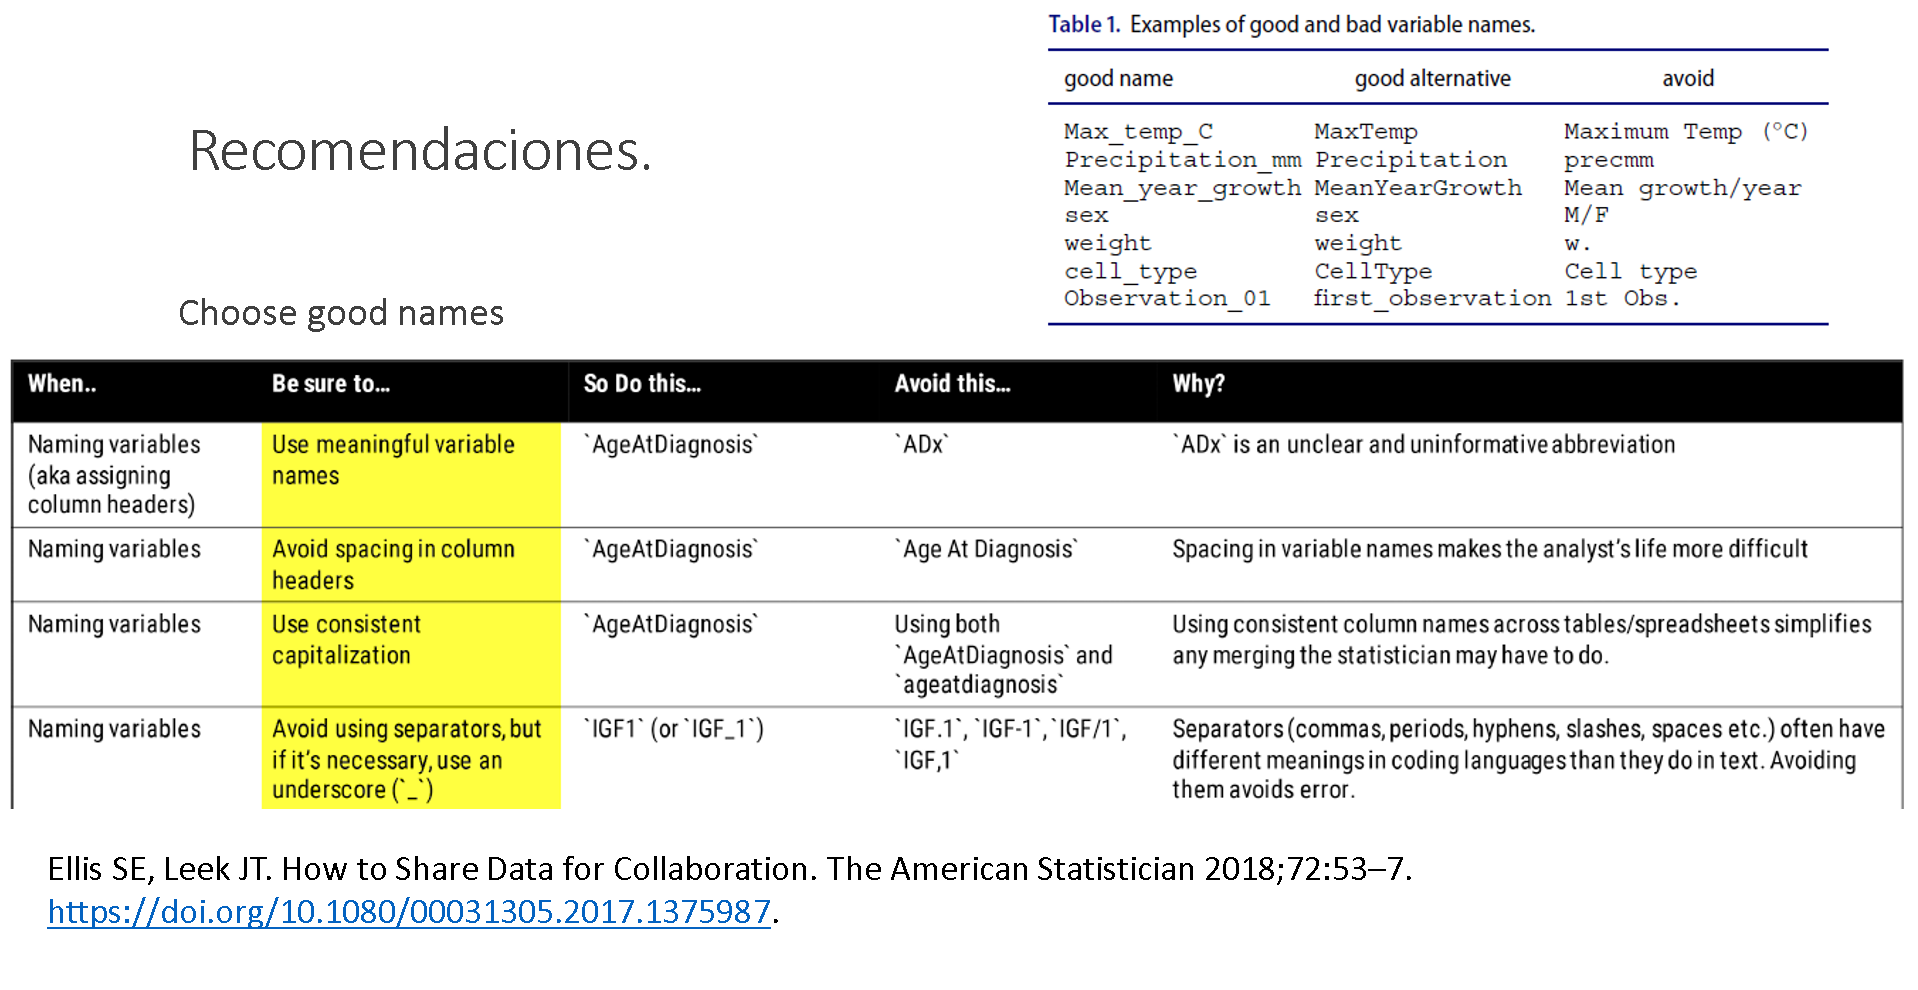
\includegraphics{./pics/Recom1.png}

\hypertarget{date-formatsnot-empty-cells.}{%
\paragraph{Date formats+not empty
cells.}\label{date-formatsnot-empty-cells.}}

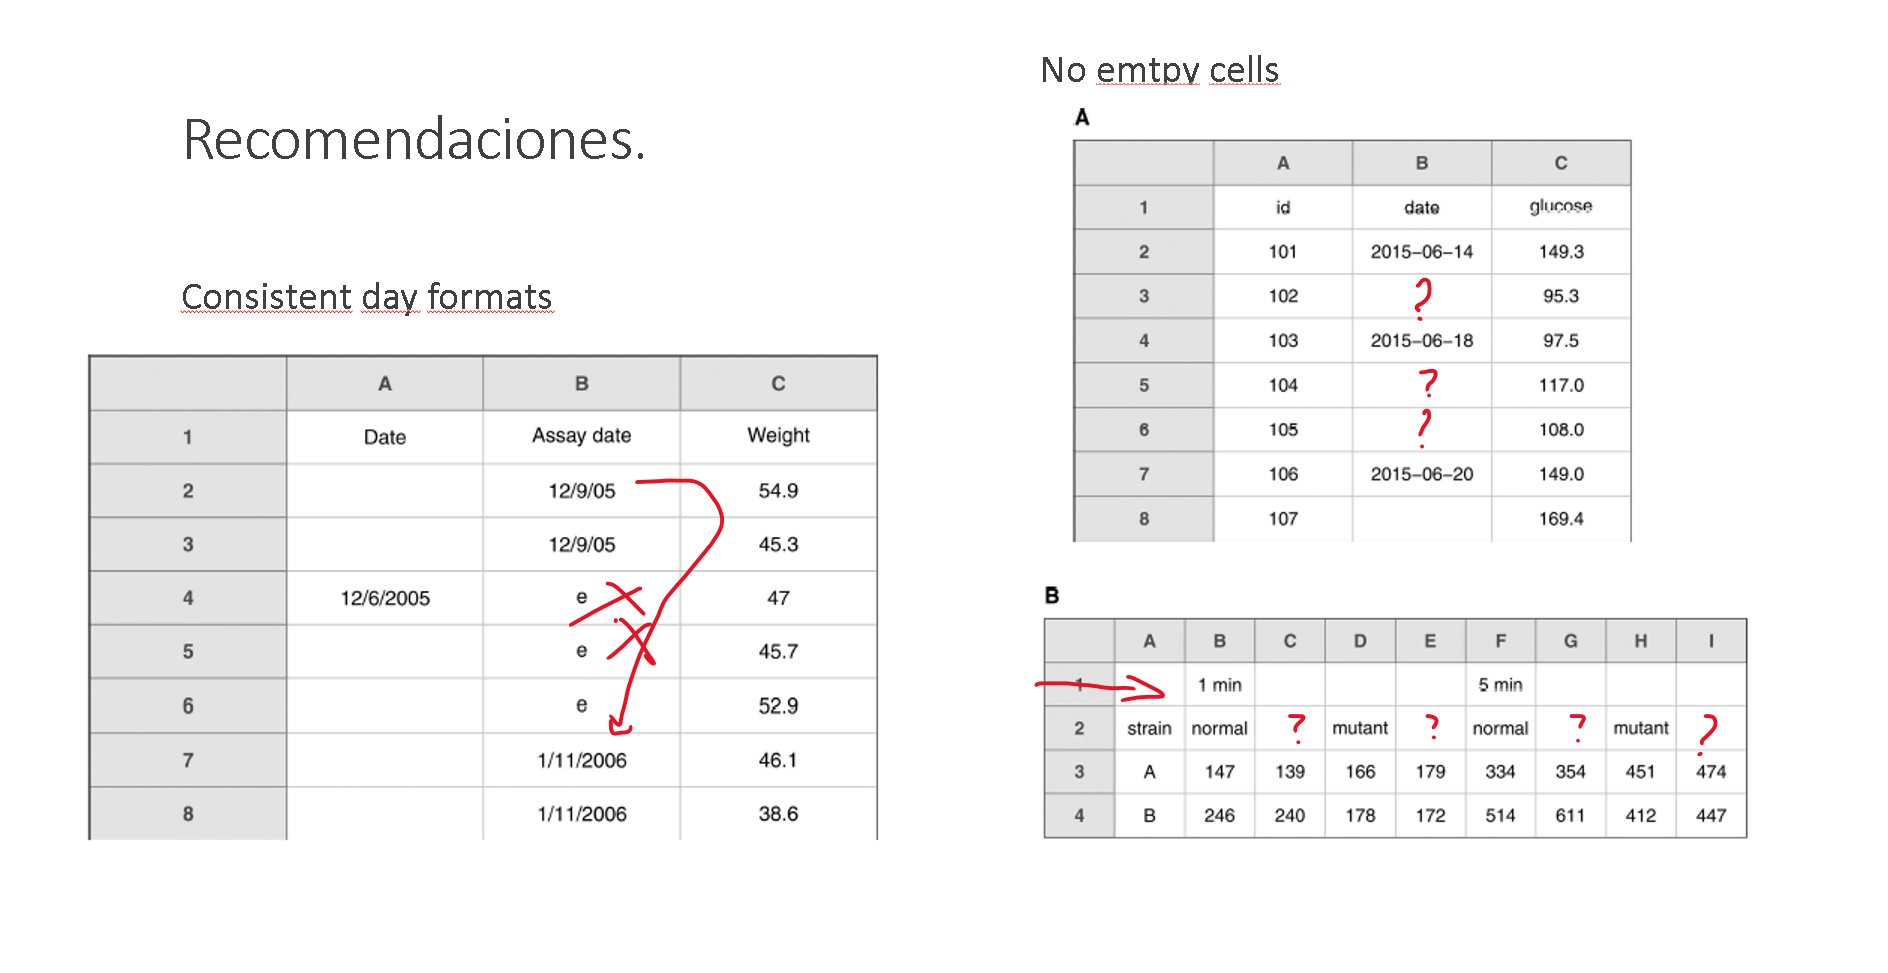
\includegraphics{./pics/Recom2.png}

\hypertarget{just-one-thing-in-a-cell-dont-use-highlighting-as-data.}{%
\paragraph{Just one thing in a cell + don´t use highlighting as
data.}\label{just-one-thing-in-a-cell-dont-use-highlighting-as-data.}}

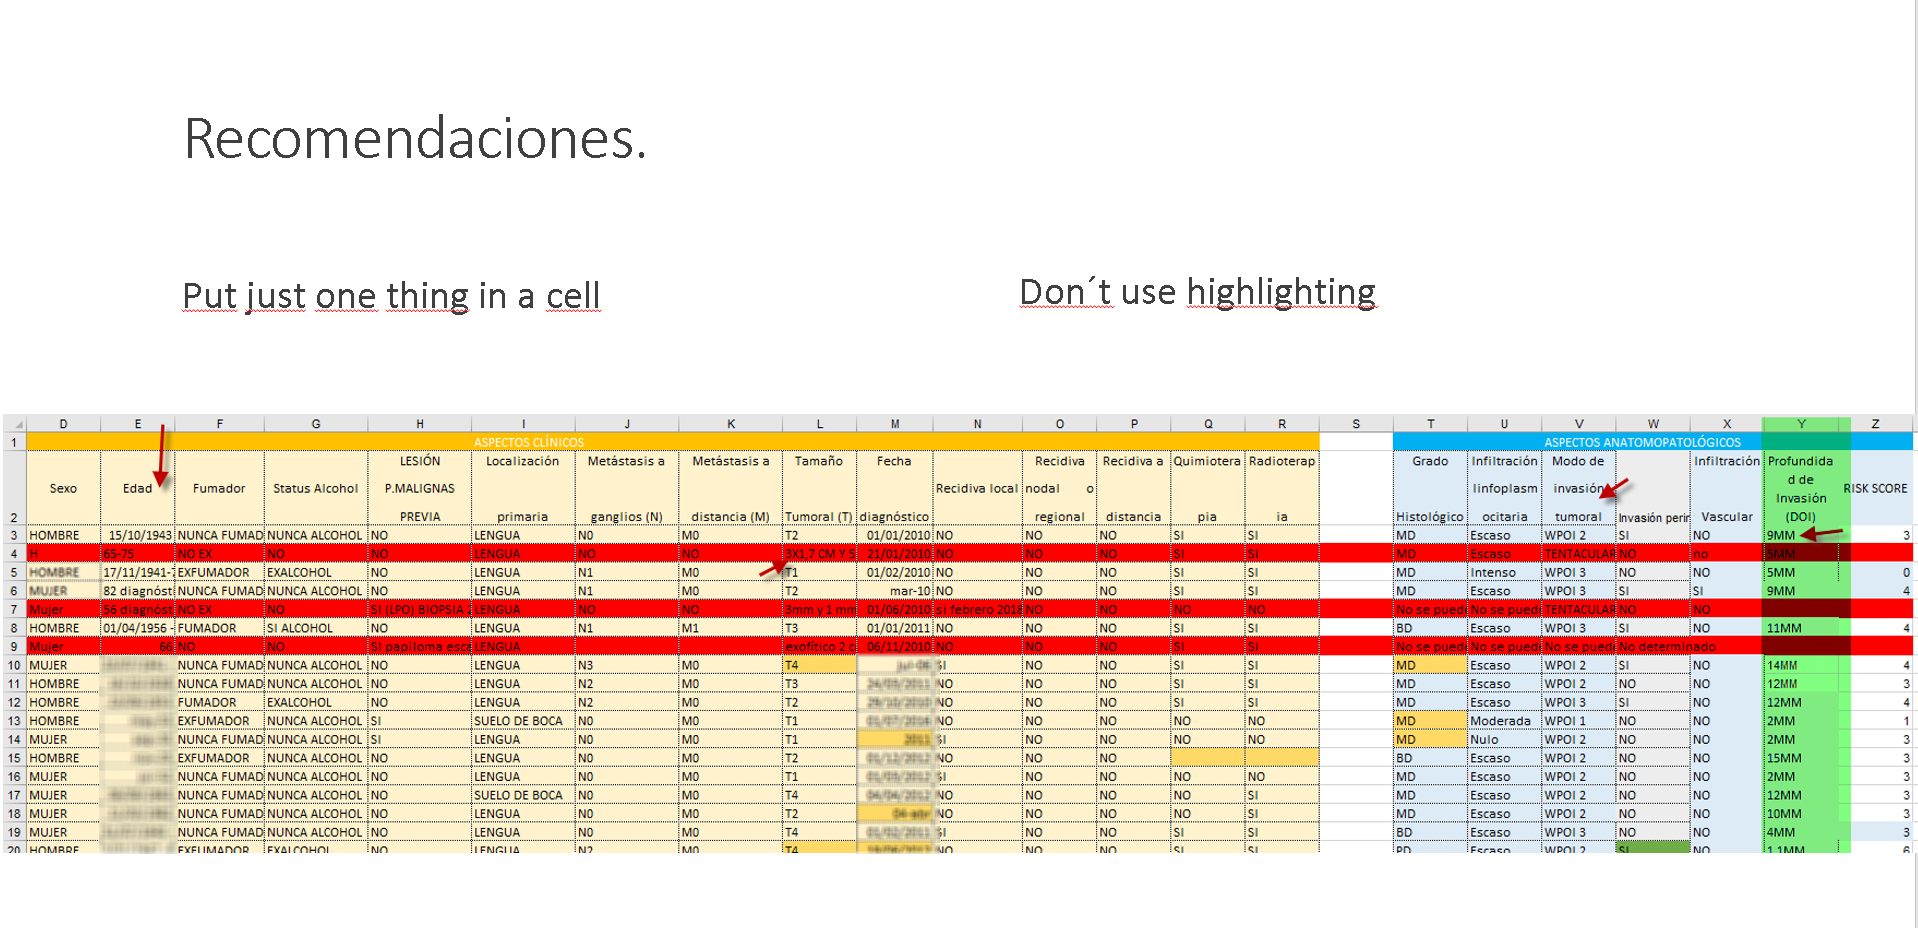
\includegraphics{./pics/Recom3.png}

\hypertarget{save-as-.csv.}{%
\paragraph{\texorpdfstring{Save as
\emph{.csv}.}{Save as .csv.}}\label{save-as-.csv.}}

Aunque es posiblemente uno de los tipos de archivo más usados para
recopilar datos, en realidad Excel está lejos de ser un programa
diseñado para este fin, y recientemente el uso de su antiguo formato
(.xls) produjo un importante error en Reino Unido al ser utilizado en la
recopilación de datos durante la pandemia por SARS-Cov2 Kelion (2020).
Aunque la culpa no era de MSExcel, cuyo formato desde 2007 (.xlsx) no
tiene la limitación del antiguo, lo cierto es que se suele recomendar
evitar su uso para recopilar datos.

Las bases de datos profesionales utilizan otros lenguajes y formatos. En
R existen paquetes que permiten importar datos de la mayoría de estas
fuentes, incluso de otros programas de análisis (SPSS, Stata, SAS\ldots)
pero, aunque no existiesen, cualquiera de ellos es capaz de exportarlos
a un pequeño archivo .csv (comma separated values), que es a su vez
importable desde todos ellos, también por R. Esto convierte al formato
\textbf{.csv} en un formato frecuente en el intercambio de datos cuando
no existe otro camino.

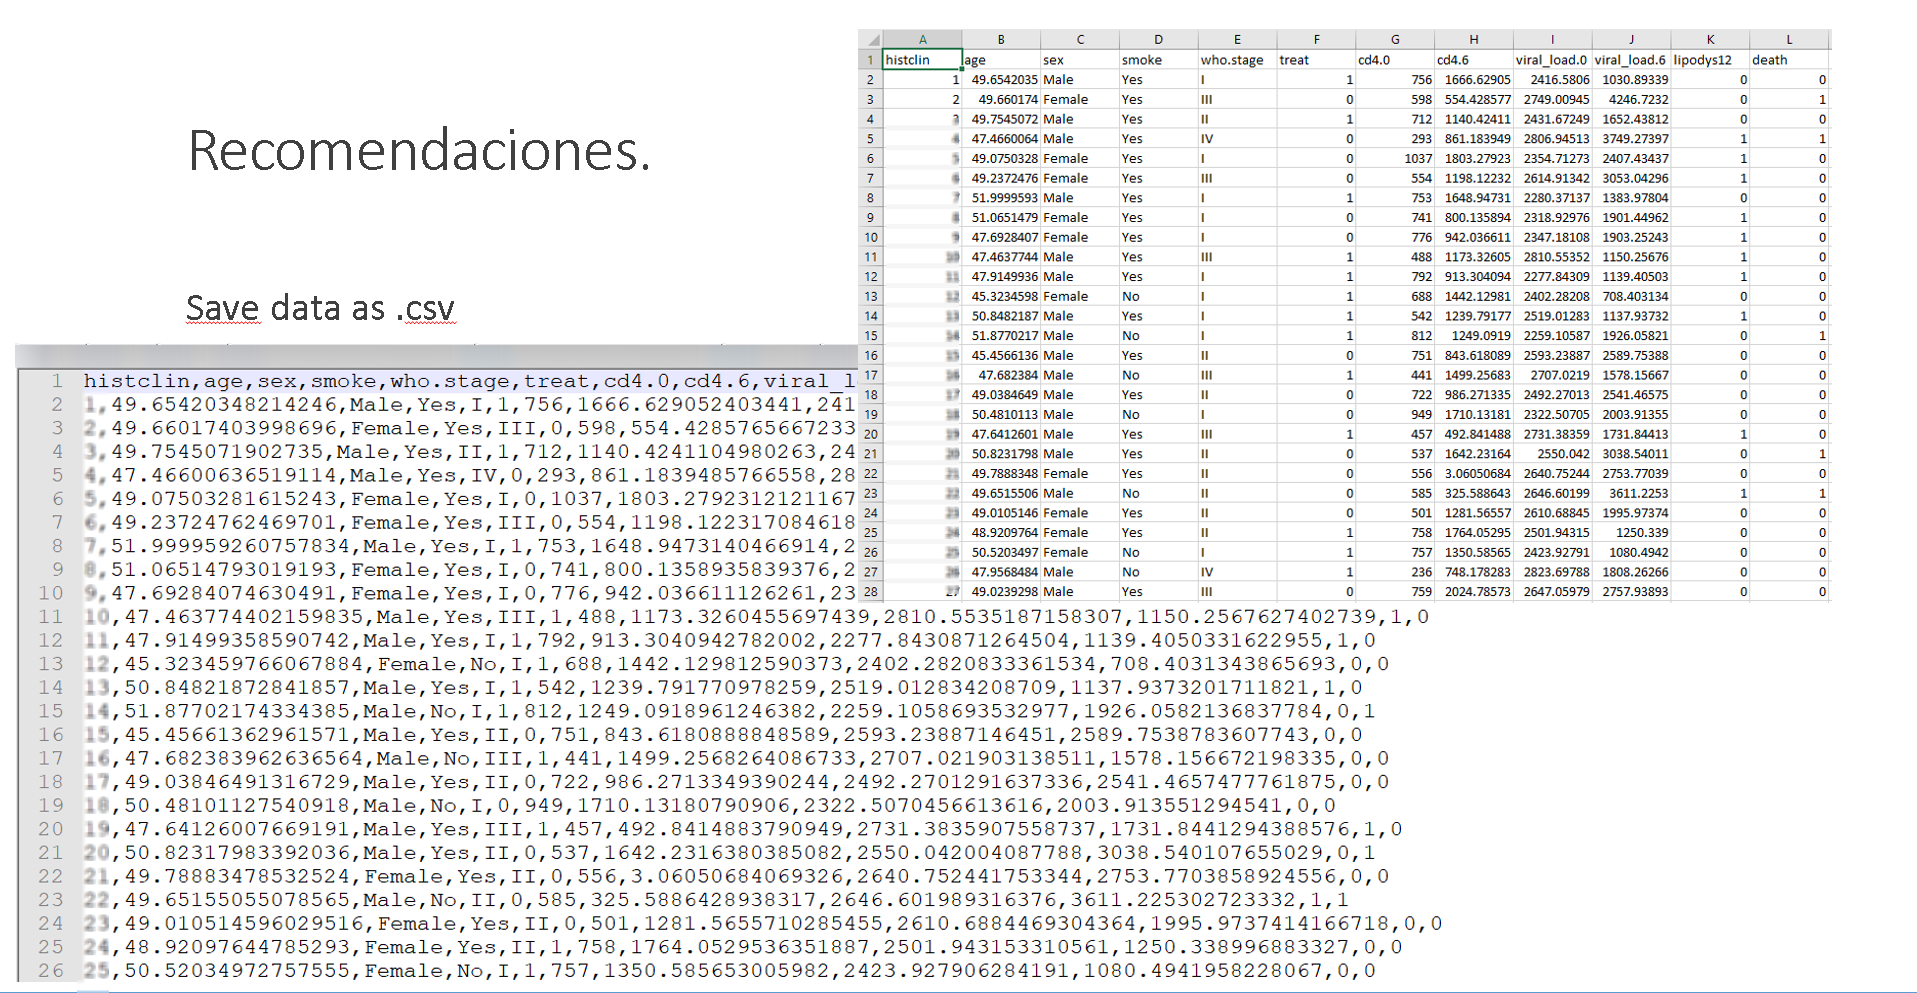
\includegraphics{./pics/Recom_save_as_csv.png}

Aunque podríamos ``crear'' y editar los datos en el propio R\footnote{Recordad
  que siempre es mejor utilizar direccionamiento relativo
  (/\_data/iam.RDS) en vez de absoluto
  (`C:/Users/Usuario/Documents/SUB1/SUB2/SUB3/SUB4/SUB5/SUB6/dataiam.RDS')
  - atención a la dirección de la barra si copiasteis el path desde
  Windows}, esto no es recomendable, entre otras cosas por la pérdida de
reproducibilidad que conlleva, y por la ausencia de controles de entrada
que sí están disponibles en las bases de datos que utilizan formularios
que permiten asegurar cierta calidad durante su introducción, por
ejemplo mediante listas desplegables que impiden introducir valores no
incluidos en ellas o mediante filtros de valor que evitan introducir
valores imposibles (p.ej. edad =999).

Dicho esto, es obvio que muchos usuarios que sabrían rellenar una hoja
de Excel (en el fondo una estructura tabular), no cuentan con
conocimientos suficientes para crear una base de datos utilizando una
estructura de tablas relacionadas, asociadas a formularios con controles
de entrada sobre consultas SQL, y tampoco cuentan con apoyo técnico para
poder hacerlo, por lo que muchos no tendrán más remedio que recurrir a
archivos .xlsx. De hacerlo, \textbf{es aún más importante seguir las
recomendaciones anteriores} de cara a facilitar su importación y reducir
los errores de introducción.

Por todo lo expuesto, lo más frecuente es que los datos crudos hayan
sido recogidos en alguno de estos formatos (también en Excel), por
nosotros mismos o por terceros, y por lo tanto debemos ser capaces de
importarlos. Esto lo veremos en siguientes sesiones.

Por último, algunos de los paquetes de R (ya veremos qué es esto)
incluyen datos que permiten seguir los ejemplos. En la siguiente sesión
también veremos cómo cargarlos (en este caso no es una importación) de
forma sencilla.

\hypertarget{referencias.}{%
\section{Referencias.}\label{referencias.}}

\bookmarksetup{startatroot}

\hypertarget{pr1-introducciuxf3n-a-r-y-rstudio.}{%
\chapter{PR1-Introducción a R y
RStudio.}\label{pr1-introducciuxf3n-a-r-y-rstudio.}}

Este documento no aborda aspectos como la instalación de R y RStudio,
aspectos bien cubiertos en muchos otros recursos, algunos mencionados en
la bibliografía.

El siguiente esquema trata de representar el flujo de trabajo habitual
en cualquier proyecto de data science independientemente de su
envergadura.

En la preparación de cualquier trabajo de investigación en el que
nosotros nos encarguemos del análisis pasaremos por todas, o casi todas,
estas fases.

En sentido estricto, el análisis estadístico sería el ciclo
Transform-Visualise-Model, pero es imposible llegar a estas fases si no
se completan los pasos anteriores.

Por otro lado, sería extraño realizar un análisis para no comunicarlo,
por lo que, aunque las siguientes notas no siguen exactamente este
esquema, es importante tratar de pensar a qué fase corresponde todo lo
que veremos en la parte práctica.

\begin{figure}

{\centering 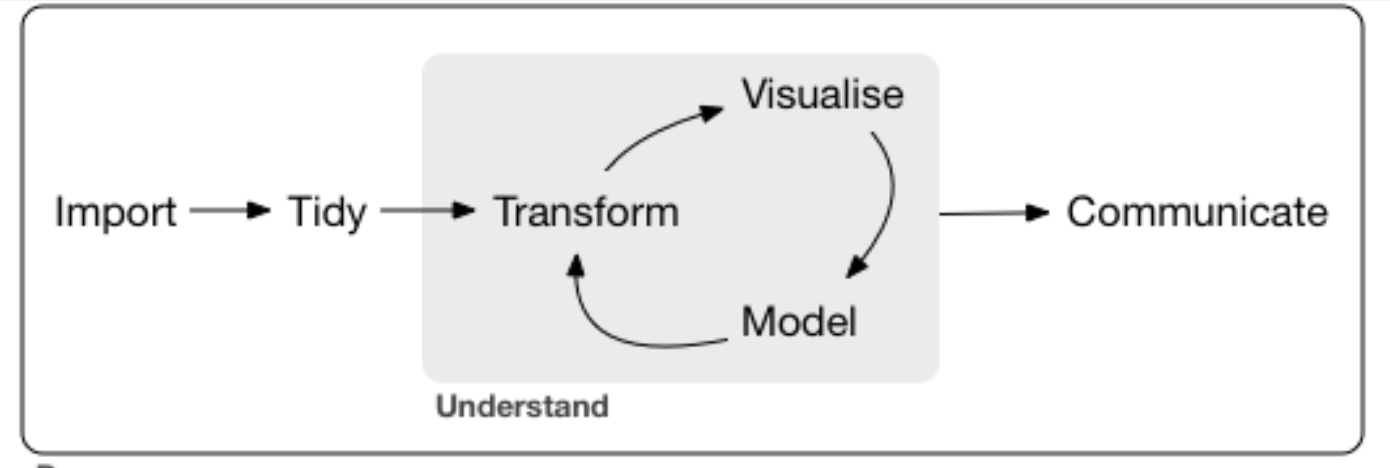
\includegraphics[width=0.5\textwidth,height=\textheight]{./pics/datascience_proj.png}

}

\caption{Data Science WorkFlow}

\end{figure}

\hypertarget{por-quuxe9-utilizar-r-para-analizar-los-datos-de-tu-investigaciuxf3n}{%
\section{¿Por qué utilizar R para analizar los datos de tu
investigación?}\label{por-quuxe9-utilizar-r-para-analizar-los-datos-de-tu-investigaciuxf3n}}

\hypertarget{ventajas}{%
\subsection{Ventajas:}\label{ventajas}}

\begin{itemize}
\tightlist
\item
  Código vs.~ventanas. (En realidad, SPSS, Stata, SAS\ldots{} también se
  pueden utilizar usando código)
\item
  Reproducibilidad (interna y externa).
\item
  Replicabilidad.
\item
  Velocidad.
\item
  Ayuda de la comunidad (software libre).
\item
  Multitud de recursos.
\item
  Nadie te acusará de estar pirateando software.
\item
  Una vez conoces los fundamentos, puedes crecer lo que desees.
\end{itemize}

\hypertarget{desventaja.}{%
\subsection{Desventaja.}\label{desventaja.}}

\begin{itemize}
\tightlist
\item
  Curva de aprendizaje lenta en comparación con las \emph{ventanas}.
\end{itemize}

\hypertarget{instalaciuxf3n-de-r-y-rstudio.}{%
\section{Instalación de R y
RStudio.}\label{instalaciuxf3n-de-r-y-rstudio.}}

Es conveniente instalar R y luego RStudio.

\begin{enumerate}
\def\labelenumi{\arabic{enumi}.}
\tightlist
\item
  Instalar R desde aquí: \url{https://cran.r-project.org/}
\item
  Instalar RStudio Desktop desde aquí: \url{https://posit.co/downloads/}
\end{enumerate}

Para detalles sobre la instalación y otros aspectos básicos,
\href{https://anabelforte.com/2022/11/20/empezando-en-r-con-rstudio/}{este
recurso} creado por Anabel Forte Deltell (más conocida como BayesAna)
\href{https://twitter.com/AnaBayes}{\includegraphics{https://img.shields.io/twitter/url/https/twitter.com/AnaBayes.svg?style=social\&label=Follow\%20\%40AnaBayes}}
es un buen punto de arranque.

\hypertarget{trabajando-con-rrstudio.}{%
\section{Trabajando con R+RStudio.}\label{trabajando-con-rrstudio.}}

\hypertarget{conceptos-buxe1sicos-para-comenzar-a-trabajar-.}{%
\subsection{Conceptos básicos para comenzar a trabajar
.}\label{conceptos-buxe1sicos-para-comenzar-a-trabajar-.}}

Aunque no en este orden, repasaremos todos estos conceptos durante la
sesión.

No hace falta que los memorices ahora. Se trata de conceptos que irás
incorporando mientras practicas con RStudio.

\begin{itemize}
\tightlist
\item
  Workspace, directorio de trabajo , Imagen (.RData).
\item
  Paneles: Console, Script,Environment/History/Connection/Tutorial .
\item
  Métodos abreviados de teclado útiles. Ctrl+Intro, Ctrl+Shift+C,
  Ctrl+Shift+N\ldots{}
\item
  Cómo instalar bibliotecas (library).
\item
  Cómo abrir o llamar a una biblioteca: \emph{require()},
  \emph{library()}.
\item
  Cómo llamar a las funciones de una biblioteca (la posición de los
  argumentos es relevante).
\item
  Organización del script: Comentar, Outline, ejecución de líneas.
\item
  Cómo pedir ayuda en Rstudio y en internet.
\end{itemize}

\begin{figure}

{\centering 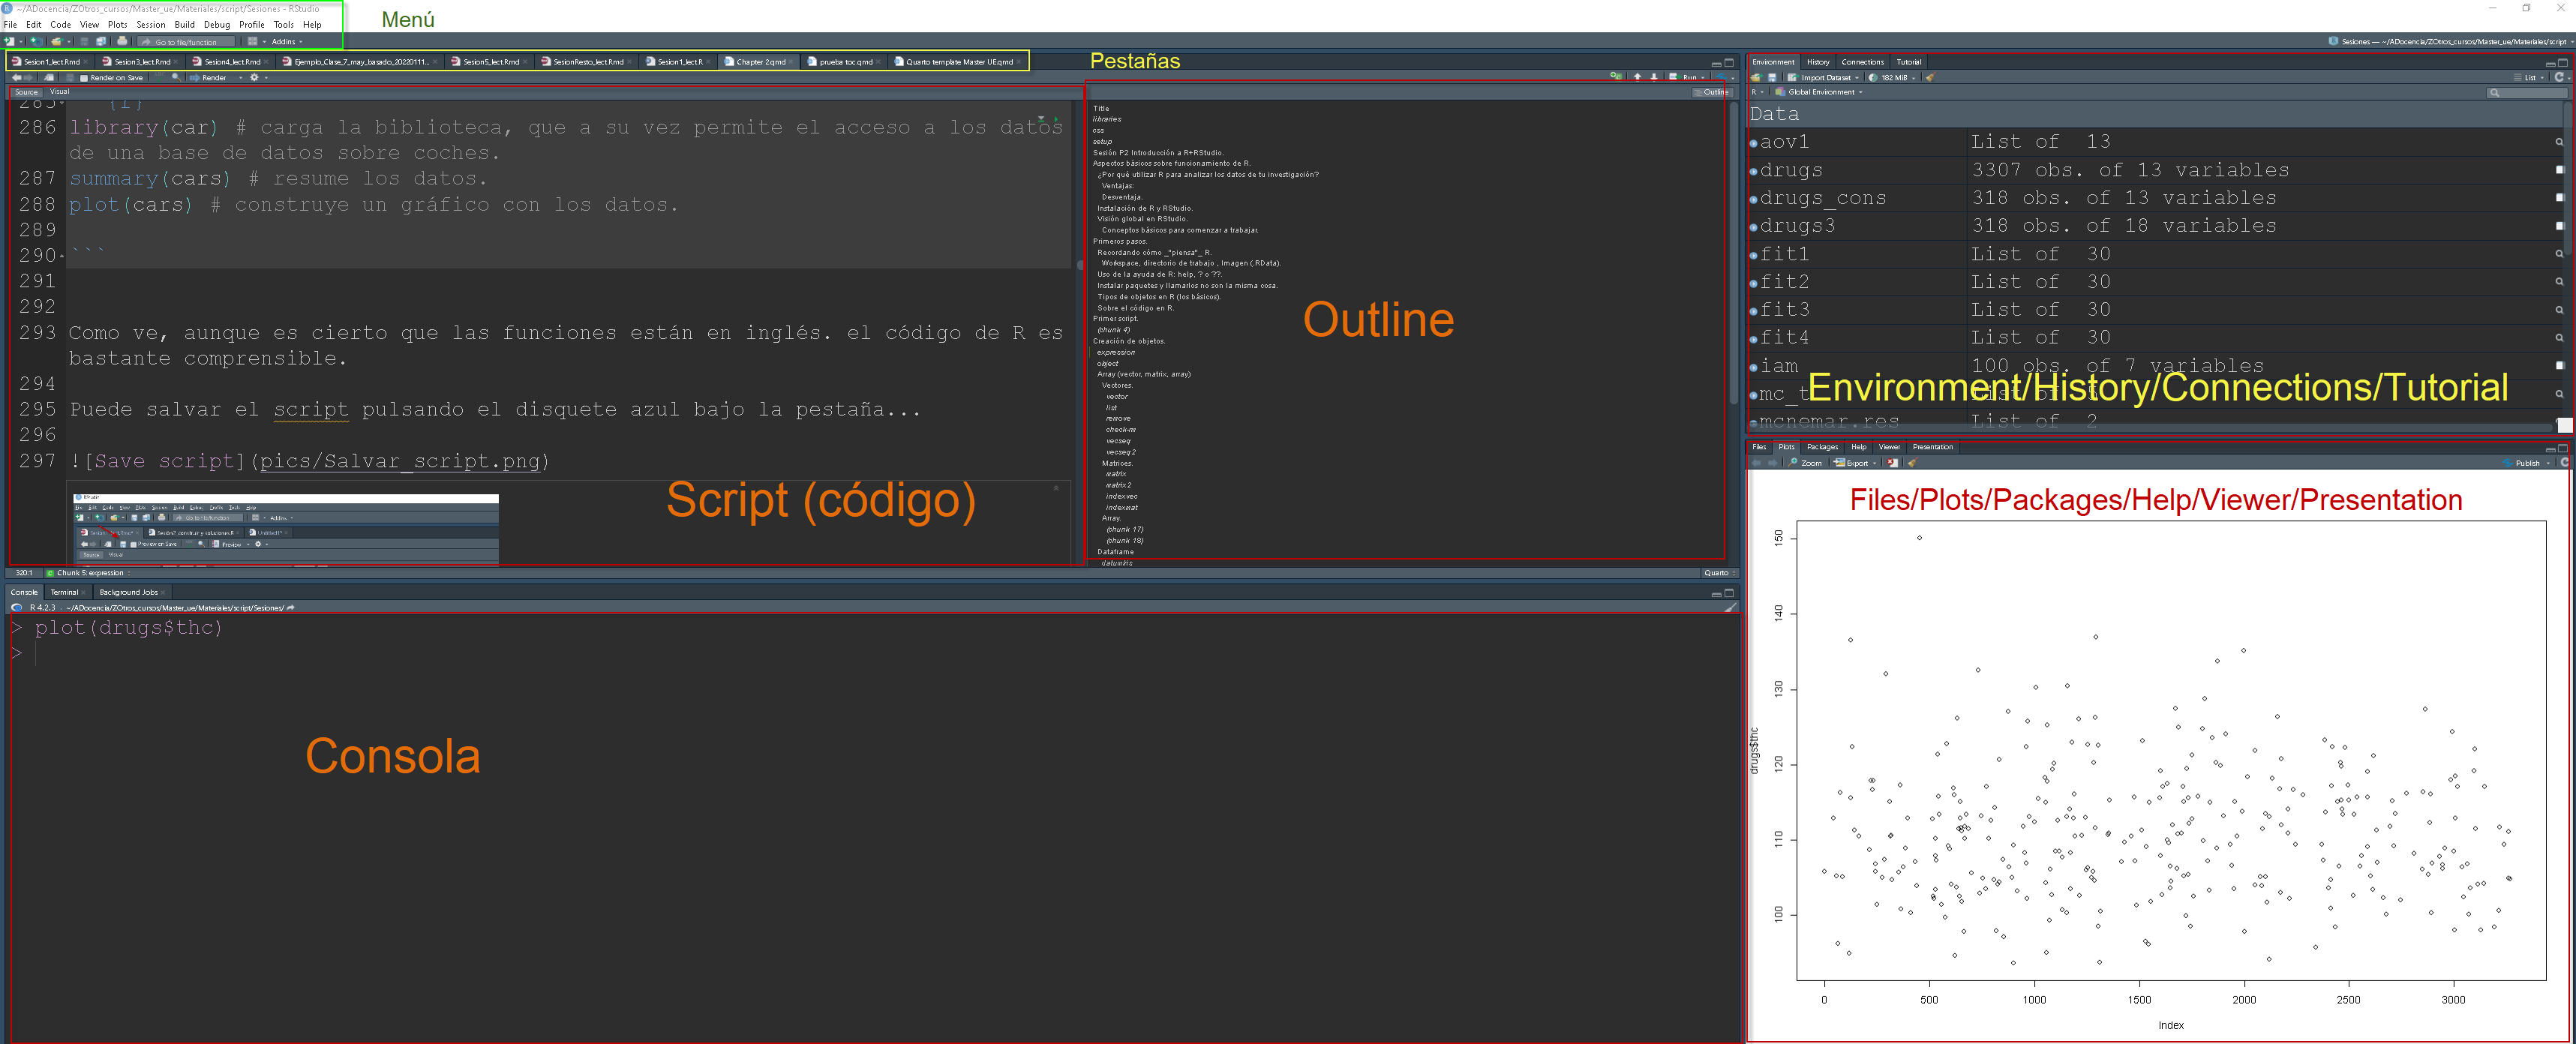
\includegraphics[width=2\textwidth,height=\textheight]{./pics/panelesRstudio.png}

}

\caption{Paneles en RStudio}

\end{figure}

\hypertarget{primeros-pasos.}{%
\subsection{Primeros pasos.}\label{primeros-pasos.}}

\hypertarget{recordando-cuxf3mo-piensa-r.}{%
\subsection{\texorpdfstring{Recordando cómo \emph{``piensa''}
R.}{Recordando cómo ``piensa'' R.}}\label{recordando-cuxf3mo-piensa-r.}}

\begin{figure}

{\centering 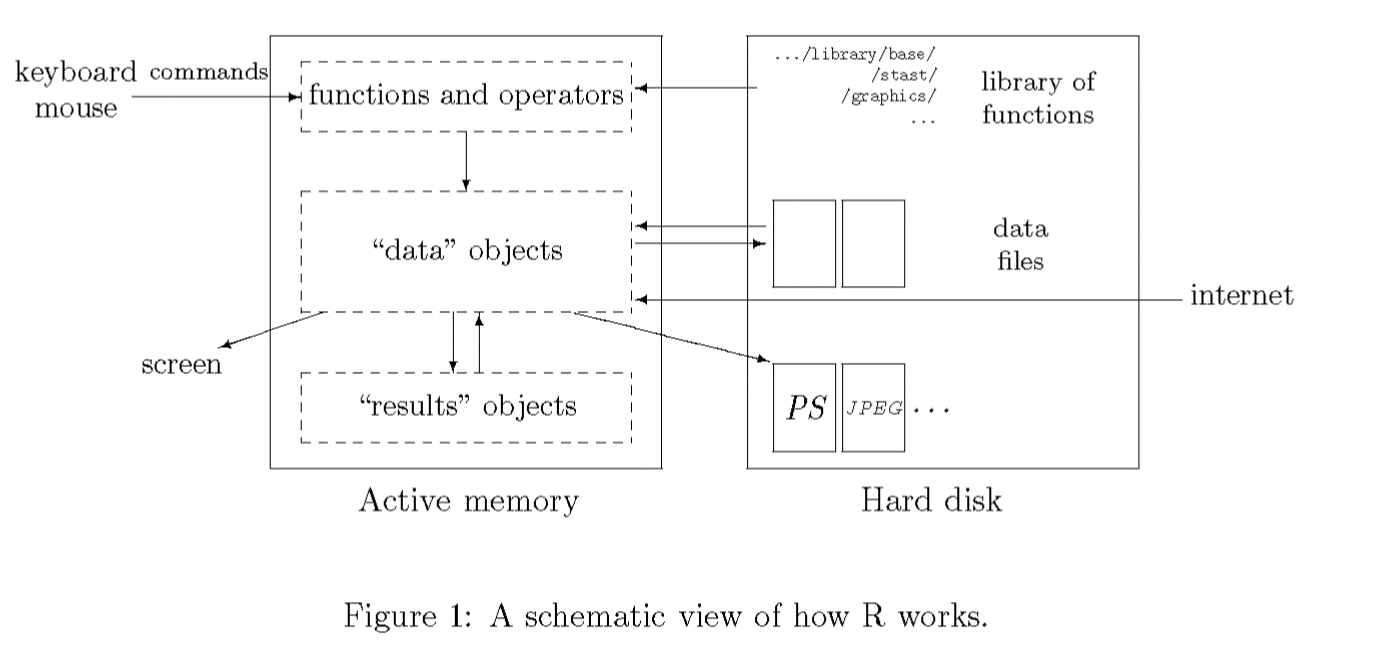
\includegraphics{./pics/como_piensa_R.png}

}

\caption{Cómo piensa R}

\end{figure}

\hypertarget{uso-de-la-ayuda-de-r-help-o-.}{%
\subsection{Uso de la ayuda de R: help, ? o
??.}\label{uso-de-la-ayuda-de-r-help-o-.}}

\begin{itemize}
\tightlist
\item
  help.start() \#Abre el navegador (solo si tenemos la ayuda html
  instalada)
\item
  help.search(``normal'') \# Busca términos relacionados.
\end{itemize}

Cómo consultar la ayuda de R:

\begin{itemize}
\tightlist
\item
  ? Consulta de ayuda para funciones.
\end{itemize}

\emph{help(stats)} es lo mismo que \emph{?stats}.

\begin{itemize}
\item
  ?? busca el texto texto en las páginas de ayuda \emph{??stats}.
\item
  Si se trata de caracteres o de expresiones reservadas porque se
  utilizan en operaciones básicas (como \emph{+}) o en el interior de
  otras funciones s (como \emph{if} ), es necesario rodear la expresión
  con ``\,'' para que devuelva la ayuda.
\item
  Correcto \emph{help(``if'') o ?``if''} vs.~Incorrecto: \emph{help(if)}
  p \emph{?if}
\end{itemize}

\hypertarget{instalar-paquetes-y-llamarlos-no-son-la-misma-cosa.}{%
\subsection{Instalar paquetes y llamarlos no son la misma
cosa.}\label{instalar-paquetes-y-llamarlos-no-son-la-misma-cosa.}}

Cuando explico este tema, suelo utilizar el ejemplo que sugieren los
nombres que vamos a utilizar, solo que en otro contexto.

Instalar la librería (\emph{install.packages(`library\_name')})
significa ir a la tienda y comprar la biblioteca (library) con los
libros incluidos.

Cargarla (\emph{library(library\_name)}) o llamarla
(\emph{require(library\_name)}) sería equivalente a abrir la librería y
ponerla a disposición del usuario.

Llamar a una de las funciones que contiene sería equivalente a utilizar
uno de los libros (\emph{function\_name(args,\ldots)}), libro que puedo
usar de muchas formas, siempre que conozca los los \emph{argumentos}
para poder hacerlo de la forma que yo deseo.

\begin{quote}
Nota:
\end{quote}

\begin{itemize}
\tightlist
\item
  Aunque no son exactamente lo mismo, escuchará library, biblioteca o
  paquete para referirse a estas bibliotecas (traducción al español de
  library).
\item
  Para utilizar las funciones anteriores, deberá sustituir
  \emph{library\_name} por el nombre de la biblioteca (\emph{library})
  que corresponda, y \emph{function\_name} por la función de dicha
  librería que desee utilizar.
\end{itemize}

Instalar un paquete implica copiar una serie de archivos en su ordenador
en una carpeta ubicada en un subdirectorio bajo la carpeta de R, es
decir es un \emph{hecho físico constatable}.

\begin{quote}
Nota: Se puede cambiar la ubicación pero de momento recomendamos que
deje a R instalarlos en la ubicación por defecto que contiene todas las
bibliotecas {[}\emph{libraries}{]}. Para ver qué librerías tenemos
instaladas, podemos utilizar la función \emph{installed.packages()}.
Verá que pueden estar en diferentes ubicaciones.
\end{quote}

Cargar la librería es ponerla en una zona de memoria que la hace
disponible, de forma que basta con llamar a las funciones. En realidad
se puede llamar a las funciones sin cargar la librería, pero deberemos
llamarla cada vez que ejecutemos una de las funciones que contenga. Para
esto se usa la expresión \emph{library\_name::function()}.

\hypertarget{tipos-de-objetos-en-r-los-buxe1sicos.}{%
\subsection{Tipos de objetos en R (los
básicos).}\label{tipos-de-objetos-en-r-los-buxe1sicos.}}

\begin{itemize}
\item
  \textbf{Escalar}.
\item
  \textbf{Array}: Agrupación multidimiensional de vectores. Todos
  elementos del mismo tipo.
\item
  \textbf{Vectores}: Numéricos, Lógicos, Cadenas, Factores. Como es
  Array-\textgreater todos elementos del mismo tipo
\item
  \textbf{Matrices (matrix)}. Array de dim=2. Como es
  Array-\textgreater todos elementos del mismo tipo.
\item
  \textbf{dataframes (data.frame)}. Matrices que pueden contener
  elementos de varios tipos, pero todos de la misma longitud.
\item
  \textbf{Listas (list)}. Elementos puedes ser de diferentes tipos y
  longitudes.
\item
  \textbf{Funciones (function)}: conjunto de código de R ejecutable y
  parametrizable.

  Nota: Todos los objetos tienen atributos length y mode. Los arrays
  además tienen dim.
\end{itemize}

\hypertarget{organizaciuxf3n-del-script.}{%
\subsection{Organización del
script.}\label{organizaciuxf3n-del-script.}}

\begin{itemize}
\item
  Las funciones se pueden separar por ``;'' o por un salto de línea.
\item
  Se puede escribir en más de una línea y se pueden agrupar ``\{\}''
  dentro de una función.
\item
  El carácter para comentar código en R es \emph{\#} \{\(Hash\)\}. Evita
  que se ejecute una o varias líneas de código, y por tanto también
  permite introducir líneas de texto que nos ayuden recordar por qué
  creamos el código de esa manera. Es lo que llamaremos ``comentar el
  código''
\item
  Es importante recordar que el código es:
\item
  Case-sensitive: Sensible a mayúsculas y minúsculas: Norm es diferente
  de norm. - Completo (multilinea): El código ha de estar completo para
  ser ejecutado
\item
  Coherente. () {[}{]}: Los paréntesis han de ser coherentes (cada
  apertura su cierre).
\item
  Cuidado con caracteres reservados: =, \$, \&, *, o prohibidos
  ä,ü,í,\ldots: Reservados para cometidos concretos, mejor evitar ñ y
  otros caracteres ``extraños''.
\end{itemize}

\hypertarget{primer-script.}{%
\section{Primer script.}\label{primer-script.}}

Abre una pestaña para crear tu primer script. Lo puedes hacer desde el
menú \emph{File/New File/R script} o con el método de teclado abreviado
\emph{Ctrl+May+N}\footnote{Recordad que siempre es mejor utilizar
  direccionamiento relativo (/\_data/iam.RDS) en vez de absoluto
  (`C:/Users/Usuario/Documents/SUB1/SUB2/SUB3/SUB4/SUB5/SUB6/dataiam.RDS')
  - atención a la dirección de la barra si copiasteis el path desde
  Windows}.

Se abrirá una pestaña que señala el nuevo script. Pega en ese espacio el
siguiente código:

\begin{Shaded}
\begin{Highlighting}[]
\FunctionTok{library}\NormalTok{(car) }\CommentTok{\# carga la biblioteca, que a su vez permite el acceso a los datos de una base de datos sobre coches.}
\end{Highlighting}
\end{Shaded}

\begin{verbatim}
Cargando paquete requerido: carData
\end{verbatim}

\begin{verbatim}

Adjuntando el paquete: 'car'
\end{verbatim}

\begin{verbatim}
The following object is masked from 'package:dplyr':

    recode
\end{verbatim}

\begin{verbatim}
The following object is masked from 'package:purrr':

    some
\end{verbatim}

\begin{Shaded}
\begin{Highlighting}[]
\FunctionTok{summary}\NormalTok{(cars) }\CommentTok{\# resume los datos.}
\end{Highlighting}
\end{Shaded}

\begin{verbatim}
     speed           dist       
 Min.   : 4.0   Min.   :  2.00  
 1st Qu.:12.0   1st Qu.: 26.00  
 Median :15.0   Median : 36.00  
 Mean   :15.4   Mean   : 42.98  
 3rd Qu.:19.0   3rd Qu.: 56.00  
 Max.   :25.0   Max.   :120.00  
\end{verbatim}

\begin{Shaded}
\begin{Highlighting}[]
\FunctionTok{plot}\NormalTok{(cars) }\CommentTok{\# construye un gráfico con los datos.}
\end{Highlighting}
\end{Shaded}

\begin{figure}[H]

{\centering 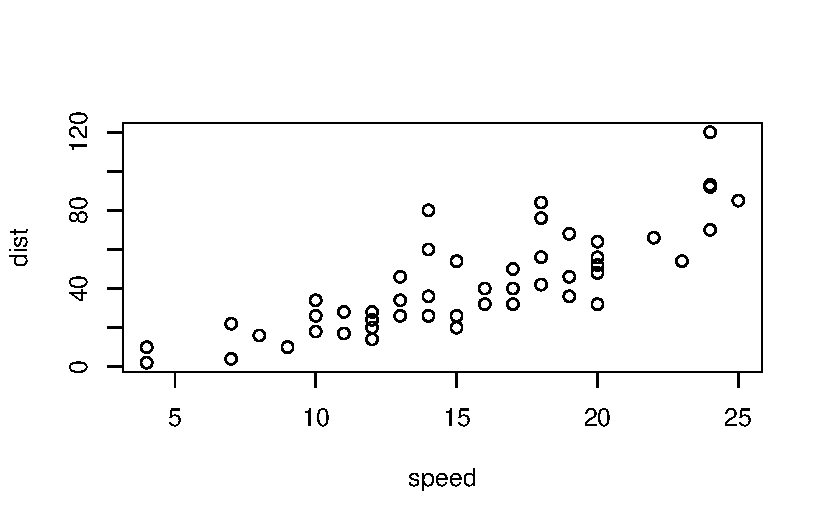
\includegraphics{./PR_1_lect_files/figure-pdf/unnamed-chunk-1-1.pdf}

}

\end{figure}

Como ves, aunque las funciones están en inglés, el código de R es
bastante comprensible para un humano.

Puede salvar el script pulsando el disquete azul bajo la pestaña\ldots{}

\begin{figure}

{\centering 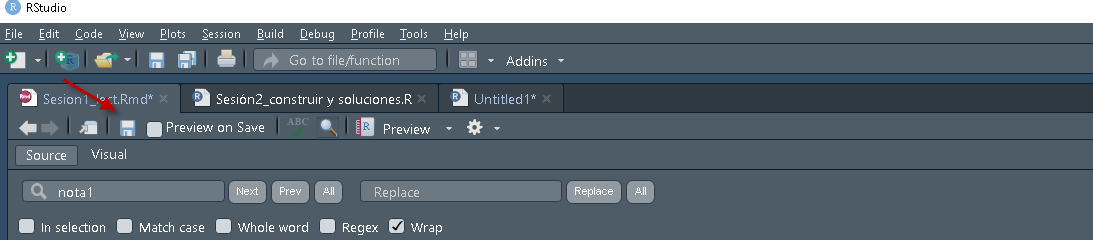
\includegraphics{./pics/Salvar_script.png}

}

\caption{Save script}

\end{figure}

\ldots{} o más fácil, con la combinación de teclas \emph{Ctrl+s}.

Las personas que utilizamos R para enseñar estadística tenemos
diferentes opiniones sobre si debemos enseñar a utilizar lo que llamamos
\emph{base R} (las funciones más básicas de R, en su mayoría incluidas
en un paquete llamado \emph{base}) o si es mejor ir directamente hacia
lo que llamamos \emph{modern R}, que utiliza algo llamado pipes
(\emph{\%\textgreater\%} o más recientemente
\emph{\textbar\textgreater{}}) que simplifica enormemente el código
necesario para realizar tareas complejas.

De hecho, aunque prácticamente todo se podría construir con rbase, el
uso del denominado \emph{tidyverse} (que incluye un conjunto de paquetes
bajo esta filosofía) agiliza mucho el trabajo, por lo que es con lo que
finalmente todos trabajamos.

\textbf{¿Merece la pena aprender algo de rbase?}

En mi opinión sí, porque aunque utilices pipes, de vez en cuando afloran
conceptos básicos. Otros profesores, en cambio, opinan que es mejor
llevar al alumnado directamente al \textbf{tidyverse} porque al final es
lo que vais a utilizar.

Nosotros pensamos que saber indexar, conocer los tipos de objetos, las
clases de vectores, etc te ayudara a entender y solucionar los problemas
que seguro aparecerán en el \textbf{tidyverse}, a descifrar los mensajes
de error y sobre todo a comprender las soluciones que encontrarás en los
blogs dedicados a este tema.

Las próximas líneas están dedicadas a mostrar algunas funciones básicos
que ayudan a comprender los diferentes objetos y estructuras con las que
vamos a trabajar, aunque luego muchas de estas funciones permanecerán
escondidas en el interior de funciones más complejas contenidas en otros
paquetes.

\hypertarget{creaciuxf3n-de-objetos.}{%
\section{Creación de objetos.}\label{creaciuxf3n-de-objetos.}}

Anteriormente hemos mencionado algunos de los objetos habitualmente
utilizados en R. Ahora vamos a aprender a crearlos.

Esto es una expresión\ldots que devuelve un resultado. No ha creado un
objeto.

\begin{Shaded}
\begin{Highlighting}[]
\DecValTok{5}\SpecialCharTok{+}\DecValTok{3}
\end{Highlighting}
\end{Shaded}

\begin{verbatim}
[1] 8
\end{verbatim}

Y esto es una asignación, que \textbf{crea un objeto} (en el ejemplo un
escalar con nombre \emph{x}), en el que almacenamos el/los resultado/s
(o la función) de, en este caso, una suma. El objeto se almacena en
memoria y se lo puede llamar en cualquier momento.

\begin{Shaded}
\begin{Highlighting}[]
\NormalTok{x}\OtherTok{\textless{}{-}}\DecValTok{5}\SpecialCharTok{+}\DecValTok{3}
\NormalTok{x}
\end{Highlighting}
\end{Shaded}

\begin{verbatim}
[1] 8
\end{verbatim}

Las funciones utilizan estos objetos para generar nuevos objetos, pero
hay algunas funciones básicas que nos ayudan a gestionar estos objetos
en nuestro espacio de trabajo\footnote{En realidad se puede comparar con
  otras distribuciones teóricas, pero la que nos interesa aquí es la
  distribución normal}.

Mencionaré tres de ellas\footnote{Si no recuerdo mal, SPSS representa
  este gráfico invirtiendo los ejes, pero la interpretación es muy
  similar.}:

\begin{itemize}
\tightlist
\item
  \emph{c()}: Concatena elementos y crea un vector, uno de los objetos
  más sencillos en R.
\item
  \emph{ls()}: Lista los objetos en el espacio de trabajo.
\item
  \emph{rm()}: Elimina objetos del espacio.
\end{itemize}

Ejemplo de uso:

\hypertarget{array-vector-matrix-array}{%
\subsubsection{Array (vector, matrix,
array)}\label{array-vector-matrix-array}}

Un array contiene un conjunto de elementos (números o caracteres) del
mismo tipo en una estructura ordenada. En función de las dimensiones
puede ser un vector (1 dimensión), una matriz (2 dimensiones) o un array
(3 dimensiones).

\textbf{Importante: Solo puede contener elementos del mismo tipo}

\hypertarget{vectores.}{%
\subsubsection{Vectores.}\label{vectores.}}

\begin{Shaded}
\begin{Highlighting}[]
\NormalTok{y}\OtherTok{\textless{}{-}}\FunctionTok{c}\NormalTok{(}\DecValTok{4}\NormalTok{,}\DecValTok{8}\NormalTok{,}\DecValTok{22}\NormalTok{,}\DecValTok{32}\NormalTok{,}\DecValTok{25}\NormalTok{) }\CommentTok{\#crea un vector de 5 elementos que son números (escalares)}
\NormalTok{y }\CommentTok{\# llamamos al objeto para que lo devuelva.}
\end{Highlighting}
\end{Shaded}

\begin{verbatim}
[1]  4  8 22 32 25
\end{verbatim}

\begin{Shaded}
\begin{Highlighting}[]
\NormalTok{nombres}\OtherTok{\textless{}{-}}\FunctionTok{c}\NormalTok{(}\StringTok{\textquotesingle{}Juan\textquotesingle{}}\NormalTok{,}\StringTok{\textquotesingle{}Luis\textquotesingle{}}\NormalTok{,}\StringTok{\textquotesingle{}Mónica\textquotesingle{}}\NormalTok{,}\StringTok{\textquotesingle{}Julia\textquotesingle{}}\NormalTok{) }\CommentTok{\#Genera un vector que contiene cadenas de caracteres.}
\NormalTok{nombres }\CommentTok{\#llamamos al objeto para que lo devuelva.}
\end{Highlighting}
\end{Shaded}

\begin{verbatim}
[1] "Juan"   "Luis"   "Mónica" "Julia" 
\end{verbatim}

\begin{verbatim}
Como se puede observar en el código anterior, hay una parte del texto detrás del carácter **#**. Todos los lenguajes de programación utilizan caracteres para "comentar" texto. El *texto comentado* no se considera parte del código, por lo que sirve para, por ejemplo, dejar explicaciones de por qué cierta parte del código se escribió de una determinada manera, o para que cierto fragmento del código no se ejecute.
\end{verbatim}

Obtener la lista de objetos en nuestro espacio de trabajo es así de
sencillo.

\begin{Shaded}
\begin{Highlighting}[]
\FunctionTok{ls}\NormalTok{()}
\end{Highlighting}
\end{Shaded}

\begin{verbatim}
[1] "nombres" "x"       "y"      
\end{verbatim}

Y eliminarlos también.

\begin{Shaded}
\begin{Highlighting}[]
\FunctionTok{rm}\NormalTok{(nombres)}
\end{Highlighting}
\end{Shaded}

Comprobamos que lo ha eliminado.

\begin{Shaded}
\begin{Highlighting}[]
\FunctionTok{ls}\NormalTok{()}
\end{Highlighting}
\end{Shaded}

\begin{verbatim}
[1] "x" "y"
\end{verbatim}

Algunas funciones nos ayudan a crear vectores de manera más rápida. Aquí
van algunos ejemplos que nos pueden ser útiles más adelante, por ejemplo
cuando hablemos de indexación:

\begin{Shaded}
\begin{Highlighting}[]
\NormalTok{a1}\OtherTok{\textless{}{-}}\FunctionTok{rep}\NormalTok{(}\DecValTok{1}\NormalTok{,}\DecValTok{20}\NormalTok{) }\CommentTok{\#Repitiendo elementos.}
\NormalTok{b}\OtherTok{\textless{}{-}}\FunctionTok{seq}\NormalTok{(}\DecValTok{1}\NormalTok{,}\DecValTok{20}\NormalTok{,}\DecValTok{2}\NormalTok{)  }\CommentTok{\# Construyendo sucesiones, por ejemplo aritmética de distancia 2 comenzando el el 1.}
\NormalTok{d}\OtherTok{\textless{}{-}}\DecValTok{27}\SpecialCharTok{:}\DecValTok{42} \CommentTok{\#cuando la distancia es uno se puede abreviar así.}
\NormalTok{vecnam.rep}\OtherTok{\textless{}{-}}\FunctionTok{rep}\NormalTok{(}\FunctionTok{c}\NormalTok{(}\StringTok{\textquotesingle{}Julia\textquotesingle{}}\NormalTok{,}\StringTok{\textquotesingle{}Óscar\textquotesingle{}}\NormalTok{),}\DecValTok{4}\NormalTok{)}
\end{Highlighting}
\end{Shaded}

Incluso podemos combinar (anidar) funciones.

\begin{Shaded}
\begin{Highlighting}[]
\NormalTok{a2}\OtherTok{\textless{}{-}}\FunctionTok{rep}\NormalTok{(}\DecValTok{1}\SpecialCharTok{:}\DecValTok{3}\NormalTok{,}\DecValTok{10}\NormalTok{) }\CommentTok{\#Repitiendo elementos}
\NormalTok{a2}
\end{Highlighting}
\end{Shaded}

\begin{verbatim}
 [1] 1 2 3 1 2 3 1 2 3 1 2 3 1 2 3 1 2 3 1 2 3 1 2 3 1 2 3 1 2 3
\end{verbatim}

\begin{Shaded}
\begin{Highlighting}[]
\CommentTok{\# En realidad estamos anidando la función seq dentro de la función rep. }
\NormalTok{a2}\FloatTok{.1} \OtherTok{\textless{}{-}} \FunctionTok{rep}\NormalTok{(}\FunctionTok{seq}\NormalTok{(}\DecValTok{1}\NormalTok{,}\DecValTok{3}\NormalTok{),}\DecValTok{10}\NormalTok{)}
\NormalTok{a2}\FloatTok{.1}
\end{Highlighting}
\end{Shaded}

\begin{verbatim}
 [1] 1 2 3 1 2 3 1 2 3 1 2 3 1 2 3 1 2 3 1 2 3 1 2 3 1 2 3 1 2 3
\end{verbatim}

\begin{Shaded}
\begin{Highlighting}[]
\NormalTok{a3}\OtherTok{\textless{}{-}}\FunctionTok{rep}\NormalTok{(}\DecValTok{1}\SpecialCharTok{:}\DecValTok{2}\NormalTok{,}\AttributeTok{each=}\DecValTok{10}\NormalTok{) }\CommentTok{\#Repitiendo elementos, pero de otra manera.}
\NormalTok{a3}
\end{Highlighting}
\end{Shaded}

\begin{verbatim}
 [1] 1 1 1 1 1 1 1 1 1 1 2 2 2 2 2 2 2 2 2 2
\end{verbatim}

Como hemos visto anteriormente, existen objetos de muchos tipos: Array,
matriz, vector (en realidad estos dos últimos son tipos de array),
lista, dataframe\ldots. Cuando se crean, almacenan y eliminan igual que
los vectores del ejemplo anterior, indepedientente de lo complejos o
grandes que sean.

\hypertarget{matrices.}{%
\subsubsection{Matrices.}\label{matrices.}}

En el siguiente ejemplo, vamos a crear una matriz. Esto nos servirá para
explicar un concepto importante, la indexación de elementos.

Creación de una matriz.

Generamos una matriz don dos columnas (a partir de los elementos calcula
las filas necesarias), llamada m1. Por defecto los elementos se van
introduciendo en la matriz columna a columna.

\begin{Shaded}
\begin{Highlighting}[]
\NormalTok{m1}\OtherTok{\textless{}{-}}\FunctionTok{matrix}\NormalTok{(}\FunctionTok{c}\NormalTok{(}\DecValTok{2}\NormalTok{,}\DecValTok{5}\NormalTok{,}\DecValTok{8}\NormalTok{,}\DecValTok{9}\NormalTok{,}\DecValTok{20}\NormalTok{,}\DecValTok{5}\NormalTok{,}\DecValTok{8}\NormalTok{,}\DecValTok{9}\NormalTok{),}\AttributeTok{ncol=}\DecValTok{2}\NormalTok{) }
\NormalTok{m1}
\end{Highlighting}
\end{Shaded}

\begin{verbatim}
     [,1] [,2]
[1,]    2   20
[2,]    5    5
[3,]    8    8
[4,]    9    9
\end{verbatim}

Pero podemos cambiar la forma en la que los introduce, basta con
utilizar un nuevo argumento \emph{byrow} para que la rellene línea a
línea.

\begin{Shaded}
\begin{Highlighting}[]
\NormalTok{m2}\OtherTok{\textless{}{-}}\FunctionTok{matrix}\NormalTok{(}\FunctionTok{c}\NormalTok{(}\DecValTok{2}\NormalTok{,}\DecValTok{5}\NormalTok{,}\DecValTok{8}\NormalTok{,}\DecValTok{9}\NormalTok{,}\DecValTok{20}\NormalTok{,}\DecValTok{5}\NormalTok{,}\DecValTok{8}\NormalTok{,}\DecValTok{9}\NormalTok{),}\AttributeTok{ncol=}\DecValTok{2}\NormalTok{,}\AttributeTok{byrow =}\NormalTok{ T) }
\NormalTok{m2}
\end{Highlighting}
\end{Shaded}

\begin{verbatim}
     [,1] [,2]
[1,]    2    5
[2,]    8    9
[3,]   20    5
[4,]    8    9
\end{verbatim}

Como se puede observar, en los bordes aparecen las coordenadas. Al ser
un objeto bidimensional el primer espacio hace referencia a la fila y el
segundo a la columna:\emph{{[}fila,columna{]}}

En el caso del vector, que solo tiene una dimensión, no habría el
elemento columna.

Pues bien, indexar un objeto significa poder llamar a subconjuntos
dentro del mismo utilizando las coordenadas.

Indexando un vector.

\begin{Shaded}
\begin{Highlighting}[]
\NormalTok{a2[}\FunctionTok{c}\NormalTok{(}\DecValTok{1}\NormalTok{,}\DecValTok{2}\NormalTok{,}\DecValTok{6}\NormalTok{)] }\CommentTok{\#extrae elementos que ocupan las posiciones 1,2 y 6 en el vector.}
\end{Highlighting}
\end{Shaded}

\begin{verbatim}
[1] 1 2 3
\end{verbatim}

\begin{Shaded}
\begin{Highlighting}[]
\NormalTok{vecnam.rep[}\FunctionTok{seq}\NormalTok{(}\DecValTok{1}\NormalTok{,}\DecValTok{8}\NormalTok{,}\DecValTok{2}\NormalTok{)] }\CommentTok{\#extrae elemantos que ocupan las posiciones del 1 a 8, pero saltando de 2 en 2 (1,3,5,7)}
\end{Highlighting}
\end{Shaded}

\begin{verbatim}
[1] "Julia" "Julia" "Julia" "Julia"
\end{verbatim}

Indexando una matriz.

La indexación también nos permite extraer una parte de una matriz. Puede
ser un conjunto de columnas, un conjunto de filas, o las celdas
\emph{({[}fila,columna){]}} que le indiquemos.

En el siguiente código se muestran varios ejemplos.

\begin{Shaded}
\begin{Highlighting}[]
\NormalTok{m1 }\CommentTok{\#Esta es la matriz que creamos anteriormente.}
\end{Highlighting}
\end{Shaded}

\begin{verbatim}
     [,1] [,2]
[1,]    2   20
[2,]    5    5
[3,]    8    8
[4,]    9    9
\end{verbatim}

\begin{Shaded}
\begin{Highlighting}[]
\NormalTok{m1[}\FunctionTok{c}\NormalTok{(}\DecValTok{1}\NormalTok{,}\DecValTok{2}\NormalTok{),] }\CommentTok{\# Extraigo filas 1 y 2}
\end{Highlighting}
\end{Shaded}

\begin{verbatim}
     [,1] [,2]
[1,]    2   20
[2,]    5    5
\end{verbatim}

\begin{Shaded}
\begin{Highlighting}[]
\NormalTok{m1[,}\FunctionTok{c}\NormalTok{(}\DecValTok{1}\NormalTok{,}\DecValTok{2}\NormalTok{)] }\CommentTok{\# Extraigo columnas 1 y 2}
\end{Highlighting}
\end{Shaded}

\begin{verbatim}
     [,1] [,2]
[1,]    2   20
[2,]    5    5
[3,]    8    8
[4,]    9    9
\end{verbatim}

\begin{Shaded}
\begin{Highlighting}[]
\NormalTok{m1[}\FunctionTok{c}\NormalTok{(}\DecValTok{3}\NormalTok{,}\DecValTok{4}\NormalTok{),}\FunctionTok{c}\NormalTok{(}\DecValTok{1}\NormalTok{,}\DecValTok{2}\NormalTok{)] }\CommentTok{\# Extraigo un subconjunto de celdas.}
\end{Highlighting}
\end{Shaded}

\begin{verbatim}
     [,1] [,2]
[1,]    8    8
[2,]    9    9
\end{verbatim}

\hypertarget{array.}{%
\subsubsection{Array.}\label{array.}}

Se pueden crear objetos con más de dimensiones, pero no vais a encontrar
muchos ejemplos en el uso habitual.

\begin{Shaded}
\begin{Highlighting}[]
\NormalTok{ar}\OtherTok{\textless{}{-}}\FunctionTok{array}\NormalTok{(}\FunctionTok{c}\NormalTok{(}\DecValTok{1}\NormalTok{,}\DecValTok{4}\NormalTok{,}\DecValTok{4}\NormalTok{,}\DecValTok{8}\NormalTok{,}\DecValTok{9}\NormalTok{,}\DecValTok{9}\NormalTok{,}\FloatTok{9.8}\NormalTok{,}\DecValTok{9}\NormalTok{,}\DecValTok{8}\NormalTok{,}\DecValTok{9}\NormalTok{,}\FloatTok{9.2}\NormalTok{,}\DecValTok{4}\NormalTok{,}\DecValTok{5}\NormalTok{,}\DecValTok{9}\NormalTok{,}\DecValTok{10}\NormalTok{,}\DecValTok{3}\NormalTok{,}\DecValTok{4}\NormalTok{,}\DecValTok{8}\NormalTok{),}\FunctionTok{c}\NormalTok{(}\DecValTok{2}\NormalTok{,}\DecValTok{3}\NormalTok{,}\DecValTok{2}\NormalTok{)) }\CommentTok{\#Esto es un array de 2 filas (primera dimension), 3 columnas (segunda dimensión), 2 bloques (tercera dimension)}
\NormalTok{ar}
\end{Highlighting}
\end{Shaded}

\begin{verbatim}
, , 1

     [,1] [,2] [,3]
[1,]    1    4    9
[2,]    4    8    9

, , 2

     [,1] [,2] [,3]
[1,]  9.8    8  9.2
[2,]  9.0    9  4.0
\end{verbatim}

Como no son de uso habitual, no profundizaré en su uso. Como podéis ver,
elementos han de ser del mismo tipo, en este caso numéricos, pero
podrían ser caracteres (texto).

\begin{Shaded}
\begin{Highlighting}[]
\NormalTok{ar2 }\OtherTok{\textless{}{-}} \FunctionTok{array}\NormalTok{(}\FunctionTok{rep}\NormalTok{(}\FunctionTok{c}\NormalTok{(}\StringTok{\textquotesingle{}red\textquotesingle{}}\NormalTok{,}\StringTok{\textquotesingle{}yellow\textquotesingle{}}\NormalTok{,}\StringTok{\textquotesingle{}green\textquotesingle{}}\NormalTok{),}\DecValTok{6}\NormalTok{),}\FunctionTok{c}\NormalTok{(}\DecValTok{2}\NormalTok{,}\DecValTok{3}\NormalTok{,}\DecValTok{2}\NormalTok{))}
\NormalTok{ar2}
\end{Highlighting}
\end{Shaded}

\begin{verbatim}
, , 1

     [,1]     [,2]    [,3]    
[1,] "red"    "green" "yellow"
[2,] "yellow" "red"   "green" 

, , 2

     [,1]     [,2]    [,3]    
[1,] "red"    "green" "yellow"
[2,] "yellow" "red"   "green" 
\end{verbatim}

Como veis ha producido un array con las mismas dimensiones pero ahora
contiene texto.

Por cierto, puede que os llame la atención que al utilizar nombres de
colores en inglés el texto aparece del color correspondiente. Esta
mejora se incluyó en una de las recientes versiones de RStudio y es
porque este vector con colores se puede utilizar al definir colores en
un gráfico\footnote{Por cierto, no es la única forma de indicar colores
  en R}

Soy consciente de que hasta aquí puede no haber visto la utilidad de lo
expuesto, pero créeme que si entiende estos conceptos, te serán de
utilidad cuando trabajes con datos.

Así llegamos un objeto clave para el análisis de datos con R: \textbf{el
dataframe}.

\hypertarget{dataframe}{%
\subsubsection{Dataframe}\label{dataframe}}

Como ya comentamos se trata de una estructura con forma de matriz (todos
los vectores han de tener la misma longitud), pero a diferencia de esta,
\textbf{un dataframe sí puede contener información de distinto tipo},
fundamentalmente números (integer o numeric), de caracteres (texto),
lógicos (TRUE/FALSE) y factores (este último será la forma en la que
recomendaremos guardar variables categóricas y por su especificidad le
dedicaremos un epígrafe propio).

El dataframe es la estructura en la que vamos a almacenar nuestros
datos, por lo que, aunque se pueden construir desde la combinación de
matrices o vectores, lo frecuente es que los construyamos importando
datos desde otros archivos (.csv, .xlsx,\ldots).

Al tratarse de una estructura matricial, le es aplicable lo que hemos
comentado sobre la indexación de matrices, pero veremos que para
\emph{llamar} a subconjuntos dentro del dataframe, podemos utilizar
otros recursos y no solo un vector de posiciones.

En vez de hacerlo así, vamos a cargar datos que ya contiene R. R
contiene muchos ejemplos de datos que van incluidos en las diferentes
librerías y a los que podemos llamar.

Uno que se usa mucho para poner ejemplos es Iris que contiene
información sobre tres especies de flores acompañadas de sus
características (longitud y anchura de pétalos y sépalos).

Para llamarlo basta con escribir esto:

\begin{Shaded}
\begin{Highlighting}[]
\FunctionTok{data}\NormalTok{(iris) }\CommentTok{\#basta con esto porque este dataset se incluye en la librería datasets que se instala por defecto en la instalación de base.}
\end{Highlighting}
\end{Shaded}

Si quisiéramos llamar a un dataset contenido dentro de otro paquete,
deberíamos hacerlo así.

\begin{Shaded}
\begin{Highlighting}[]
\FunctionTok{data}\NormalTok{(Anscombe,}\AttributeTok{package=}\StringTok{\textquotesingle{}carData\textquotesingle{}}\NormalTok{) }
\end{Highlighting}
\end{Shaded}

La primera vez que cargamos unos datos de esta manera, en el entorno
(pestaña Environment del panel superior derecho {[}si no se ha cambiado
la colocación de los paneles en las opciones de RStudio{]}) aparecerá el
nombre en el apartado `Values' y al lado junto con el resto de objetos
que hemos ido creando.

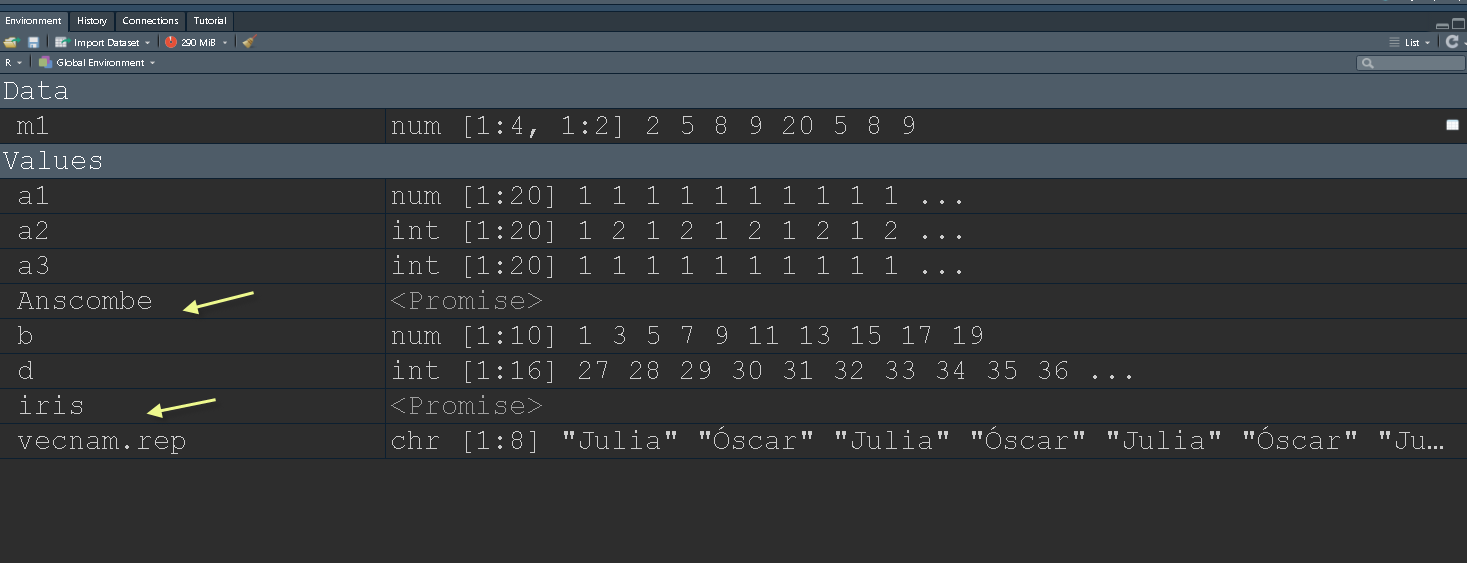
\includegraphics{./pics/Promise.png}

Si está en Promise, el dataset todavía no está cargado. Para que cargue
hemos de llamarlo una primera vez.

\begin{Shaded}
\begin{Highlighting}[]
\FunctionTok{head}\NormalTok{(iris) }\CommentTok{\# solo pedimos los primeros registros (son 50)}
\end{Highlighting}
\end{Shaded}

\begin{verbatim}
  Sepal.Length Sepal.Width Petal.Length Petal.Width Species
1          5.1         3.5          1.4         0.2  setosa
2          4.9         3.0          1.4         0.2  setosa
3          4.7         3.2          1.3         0.2  setosa
4          4.6         3.1          1.5         0.2  setosa
5          5.0         3.6          1.4         0.2  setosa
6          5.4         3.9          1.7         0.4  setosa
\end{verbatim}

\begin{Shaded}
\begin{Highlighting}[]
\FunctionTok{head}\NormalTok{(Anscombe) }
\end{Highlighting}
\end{Shaded}

\begin{verbatim}
   education income young urban
ME       189   2824 350.7   508
NH       169   3259 345.9   564
VT       230   3072 348.5   322
MA       168   3835 335.3   846
RI       180   3549 327.1   871
CT       193   4256 341.0   774
\end{verbatim}

Y es entonces cuando pasa al conjunto \emph{Data}.

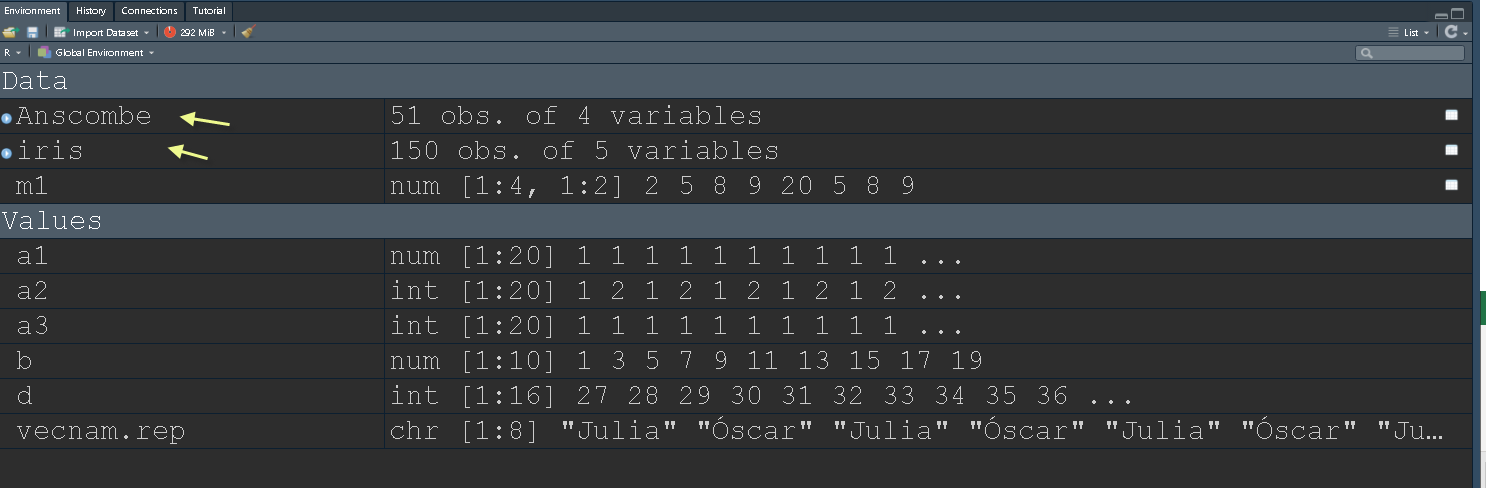
\includegraphics{./pics/Promise2.png}

En algunos ejemplos utilizaremos estos datos \emph{``precargados''} en
R, de ahí la explicación anterior, pero en general los datos serán
importados desde archivos externos.

Como comentábamos, el dataframe puede indexarse como hacíamos con la
matriz.

Solo columnas 2 y 3 de las primeras 6 filas. Las 6 filas las impone
\emph{head} por defecto. Sin usar \emph{head()}, mostraría todas.

\begin{Shaded}
\begin{Highlighting}[]
\FunctionTok{head}\NormalTok{(iris[,}\DecValTok{2}\SpecialCharTok{:}\DecValTok{3}\NormalTok{])}
\end{Highlighting}
\end{Shaded}

\begin{verbatim}
  Sepal.Width Petal.Length
1         3.5          1.4
2         3.0          1.4
3         3.2          1.3
4         3.1          1.5
5         3.6          1.4
6         3.9          1.7
\end{verbatim}

Seleccionamos los registros (ejemplares) 4 y 10, y las colunas 2 y 3 del
datarame.

\begin{Shaded}
\begin{Highlighting}[]
\NormalTok{iris[}\FunctionTok{c}\NormalTok{(}\DecValTok{4}\NormalTok{,}\DecValTok{10}\NormalTok{),}\DecValTok{2}\SpecialCharTok{:}\DecValTok{3}\NormalTok{] }\CommentTok{\#}
\end{Highlighting}
\end{Shaded}

\begin{verbatim}
   Sepal.Width Petal.Length
4          3.1          1.5
10         3.1          1.5
\end{verbatim}

Al tratarse de un dataframe, podemos llamar a las columnas, en última
instancia las variables contenidas en nuestro dataset, por su nombre.
Para ello utilizaremos un vectore de cadenas de texto (character).

\begin{Shaded}
\begin{Highlighting}[]
\NormalTok{iris[}\FunctionTok{c}\NormalTok{(}\DecValTok{4}\NormalTok{,}\DecValTok{10}\NormalTok{),}\FunctionTok{c}\NormalTok{(}\StringTok{"Sepal.Width"}\NormalTok{,}\StringTok{"Sepal.Length"}\NormalTok{)]}
\end{Highlighting}
\end{Shaded}

\begin{verbatim}
   Sepal.Width Sepal.Length
4          3.1          4.6
10         3.1          4.9
\end{verbatim}

Otra forma de llamar a una variable concreta es utilizando el carácter
reservado \emph{\$}. Para ello comenzamos con el nombre del dataframe y
separadmos el nombre de la variable mediante el símbolo del \$.

\begin{verbatim}
En realidad esta forma de llamar a partes de un objeto (utilizando $ como separador), se utiliza también en otros objetos más complejos.
\end{verbatim}

\begin{Shaded}
\begin{Highlighting}[]
\NormalTok{iris}\SpecialCharTok{$}\NormalTok{Sepal.Length}
\end{Highlighting}
\end{Shaded}

\begin{verbatim}
  [1] 5.1 4.9 4.7 4.6 5.0 5.4 4.6 5.0 4.4 4.9 5.4 4.8 4.8 4.3 5.8 5.7 5.4 5.1
 [19] 5.7 5.1 5.4 5.1 4.6 5.1 4.8 5.0 5.0 5.2 5.2 4.7 4.8 5.4 5.2 5.5 4.9 5.0
 [37] 5.5 4.9 4.4 5.1 5.0 4.5 4.4 5.0 5.1 4.8 5.1 4.6 5.3 5.0 7.0 6.4 6.9 5.5
 [55] 6.5 5.7 6.3 4.9 6.6 5.2 5.0 5.9 6.0 6.1 5.6 6.7 5.6 5.8 6.2 5.6 5.9 6.1
 [73] 6.3 6.1 6.4 6.6 6.8 6.7 6.0 5.7 5.5 5.5 5.8 6.0 5.4 6.0 6.7 6.3 5.6 5.5
 [91] 5.5 6.1 5.8 5.0 5.6 5.7 5.7 6.2 5.1 5.7 6.3 5.8 7.1 6.3 6.5 7.6 4.9 7.3
[109] 6.7 7.2 6.5 6.4 6.8 5.7 5.8 6.4 6.5 7.7 7.7 6.0 6.9 5.6 7.7 6.3 6.7 7.2
[127] 6.2 6.1 6.4 7.2 7.4 7.9 6.4 6.3 6.1 7.7 6.3 6.4 6.0 6.9 6.7 6.9 5.8 6.8
[145] 6.7 6.7 6.3 6.5 6.2 5.9
\end{verbatim}

Esto será muy útil para crear nuevas variables en el dataframe. Aunque
lo veremos con más detenimiento en la siguiente sesión, incluyo aquí
algún ejemplo básico porque ayuda a entender cómo funciona en el
dataframe.

Por ejemplo, imaginemos que deseamos crear la razón entre la longitud y
la anchura de los sépalos.

\begin{Shaded}
\begin{Highlighting}[]
\NormalTok{iris}\SpecialCharTok{$}\NormalTok{Sepal.Ratio }\OtherTok{\textless{}{-}}\NormalTok{ iris}\SpecialCharTok{$}\NormalTok{Sepal.Length}\SpecialCharTok{/}\NormalTok{iris}\SpecialCharTok{$}\NormalTok{Sepal.Width}
\end{Highlighting}
\end{Shaded}

Como podemos observar, el dataframe iris contiene ahora una nueva
variable llamada \textbf{sepal.ratio}.

\begin{Shaded}
\begin{Highlighting}[]
\NormalTok{iris[}\DecValTok{1}\SpecialCharTok{:}\DecValTok{4}\NormalTok{,}\FunctionTok{c}\NormalTok{(}\StringTok{"Sepal.Length"}\NormalTok{,}\StringTok{"Sepal.Width"}\NormalTok{,}\StringTok{"Sepal.Ratio"}\NormalTok{)] }\CommentTok{\#limito el número de filas utilizando un vector como índice.}
\end{Highlighting}
\end{Shaded}

\begin{verbatim}
  Sepal.Length Sepal.Width Sepal.Ratio
1          5.1         3.5    1.457143
2          4.9         3.0    1.633333
3          4.7         3.2    1.468750
4          4.6         3.1    1.483871
\end{verbatim}

Para eliminar una variable del data frame, basta con que asignemos NULL
al vector correspondiente.

\begin{Shaded}
\begin{Highlighting}[]
\NormalTok{iris}\SpecialCharTok{$}\NormalTok{Sepal.Ratio}\OtherTok{\textless{}{-}}\ConstantTok{NULL}
\end{Highlighting}
\end{Shaded}

Una vez hemos visto lo básico sobre cómo manejarse con un dataframe, en
la siguiente sesión aprenderemos a importar uno.

\hypertarget{listas.}{%
\subsubsection{Listas.}\label{listas.}}

La \emph{lista} es un objeto que a pesar de su utilidad cuesta
comprender cuando estás empezando a trabajar con R. En cierto modo es un
contenedor porque puede almacenar otros objetos de diferente tipo
(vectores, arrays, dataframes, gráficos) en su interior. Además, en
muchas funciones, alguno de los argumentos es de tipo lista y muchas
otras devuelven objetos de tipo lista.

¿Se puede vivir sin comprender qué es una lista en R? Sí, pero no
manejarse algo con ellas limita mucho tu crecimiento posterior. En un
curso de iniciación como este, solo pondré un ejemplo para ilustrar su
funcionamiento, pero no te preocupes si en este momento no comprendes
del todo su funcionamiento.

En este ejemplo voy a generar un vector, una matriz, un dataframe y un
gráfico\footnote{Guardar gráficos base R implica abrir el dispositivo
  gráfico y utilizar otra función, incluso la propia ayuda recomienda no
  utilizarlo para almacenar gráficos. Es más fácil utilizando los
  gráficos generados con ggplot. No hace falta saber hacerlo, pero lo
  incluyo para demostrar la versatilidad de las listas para recopilar
  objetos} y los voy a incluir en una lista.

\begin{verbatim}
En el ejemplo voy a utilizar funciones para generar vectores aleatorios siguiendo distribuciones de probabilidad teórica concretas (en el ejemplo una normal y una binomial). No es necesario entender su funcionamiento para comprender el ejemplo, basta con saber que crean vectores de 50 elementos que serán  las variables del dataframe simulado.
\end{verbatim}

\begin{Shaded}
\begin{Highlighting}[]
\NormalTok{v1 }\OtherTok{\textless{}{-}} \FunctionTok{c}\NormalTok{(}\StringTok{\textquotesingle{}Juan\textquotesingle{}}\NormalTok{, }\StringTok{\textquotesingle{}Pedro\textquotesingle{}}\NormalTok{,}\StringTok{\textquotesingle{}Luisa\textquotesingle{}}\NormalTok{)}
\NormalTok{m1 }\OtherTok{\textless{}{-}} \FunctionTok{matrix}\NormalTok{(}\FunctionTok{c}\NormalTok{(}\DecValTok{3}\NormalTok{,}\DecValTok{5}\NormalTok{,}\DecValTok{7}\NormalTok{,}\DecValTok{22}\NormalTok{,}\DecValTok{45}\NormalTok{,}\DecValTok{76}\NormalTok{,}\DecValTok{25}\NormalTok{,}\DecValTok{22}\NormalTok{,}\DecValTok{21}\NormalTok{),}\AttributeTok{ncol=}\DecValTok{3}\NormalTok{)}
\NormalTok{df1 }\OtherTok{\textless{}{-}} \FunctionTok{data.frame}\NormalTok{(}\AttributeTok{id=}\DecValTok{1001}\SpecialCharTok{:}\DecValTok{1050}\NormalTok{,}\AttributeTok{pas=}\FunctionTok{round}\NormalTok{(}\FunctionTok{rnorm}\NormalTok{(}\DecValTok{50}\NormalTok{,}\DecValTok{120}\NormalTok{,}\DecValTok{5}\NormalTok{)),}\AttributeTok{sex=}\FunctionTok{factor}\NormalTok{(}\FunctionTok{rbinom}\NormalTok{(}\DecValTok{50}\NormalTok{,}\DecValTok{1}\NormalTok{,.}\DecValTok{35}\NormalTok{),}\AttributeTok{labels=}\FunctionTok{c}\NormalTok{(}\StringTok{\textquotesingle{}Hombre\textquotesingle{}}\NormalTok{,}\StringTok{\textquotesingle{}Mujer\textquotesingle{}}\NormalTok{)))}

\FunctionTok{plot.new}\NormalTok{()}
\FunctionTok{barplot}\NormalTok{(}\FunctionTok{table}\NormalTok{(df1}\SpecialCharTok{$}\NormalTok{sex))}
\end{Highlighting}
\end{Shaded}

\begin{figure}[H]

{\centering 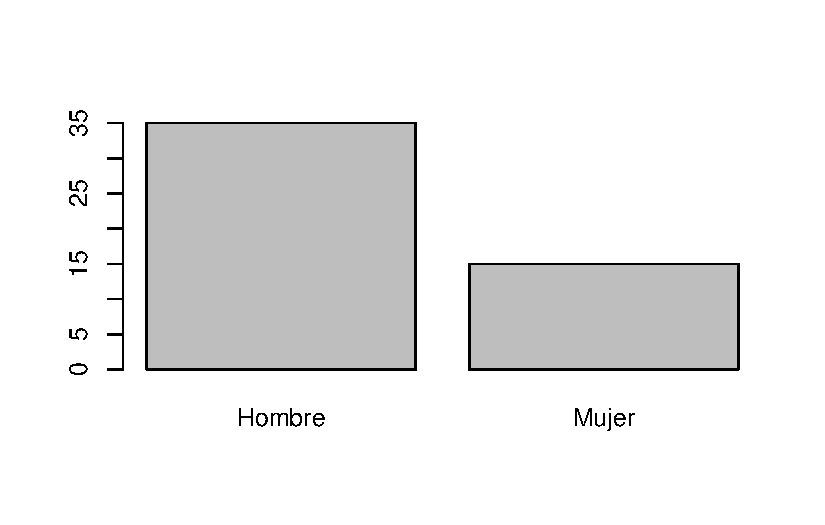
\includegraphics{./PR_1_lect_files/figure-pdf/unnamed-chunk-4-1.pdf}

}

\end{figure}

\begin{Shaded}
\begin{Highlighting}[]
\NormalTok{p1 }\OtherTok{\textless{}{-}} \FunctionTok{recordPlot}\NormalTok{()}

\NormalTok{lista1 }\OtherTok{\textless{}{-}} \FunctionTok{list}\NormalTok{(v1,m1,df1,p1)}
\end{Highlighting}
\end{Shaded}

Si analizamos su estructura, vemos que tiene cuatro elementos.

\begin{verbatim}
Utilizo el argumento max.level para limitar la información que muestra sobre la lista. El tercer elemento es muy grande y si lo muestra entero ocuparía mucho espacio. De hecho, como se puede ver, ha convertido el gráfico en ¡otra lista!
\end{verbatim}

\begin{Shaded}
\begin{Highlighting}[]
\FunctionTok{str}\NormalTok{(lista1,}\AttributeTok{max.level =} \DecValTok{1}\NormalTok{) }
\end{Highlighting}
\end{Shaded}

\begin{verbatim}
List of 4
 $ : chr [1:3] "Juan" "Pedro" "Luisa"
 $ : num [1:3, 1:3] 3 5 7 22 45 76 25 22 21
 $ :'data.frame':   50 obs. of  3 variables:
 $ :List of 3
  ..- attr(*, "engineVersion")= int 16
  ..- attr(*, "pid")= int 12188
  ..- attr(*, "Rversion")=Classes 'R_system_version', 'package_version', 'numeric_version'  hidden list of 1
  ..- attr(*, "load")= chr(0) 
  ..- attr(*, "attach")= chr(0) 
  ..- attr(*, "class")= chr "recordedplot"
\end{verbatim}

Como inica la estructura, es una lista de 4 elementos, el vector, una
matriz 3x3, un dataframe de 50 observaciones y tres variables , y un
cuarto elemento que es otra lista y que al ser llamado, devolverá el
gráfico.

Una vez creada, podemos acceder (llamar) a los elementos de la lista
utilizando índices, pero las listas necesitan doble corchete
(\textbf{{[}{[}{]}{]}}) para ser indexadas.

\begin{Shaded}
\begin{Highlighting}[]
\NormalTok{lista1[[}\DecValTok{4}\NormalTok{]] }\CommentTok{\#Esto llamaría al cuarto elemento de la lista, que era el gráfico.}
\end{Highlighting}
\end{Shaded}

\begin{figure}[H]

{\centering 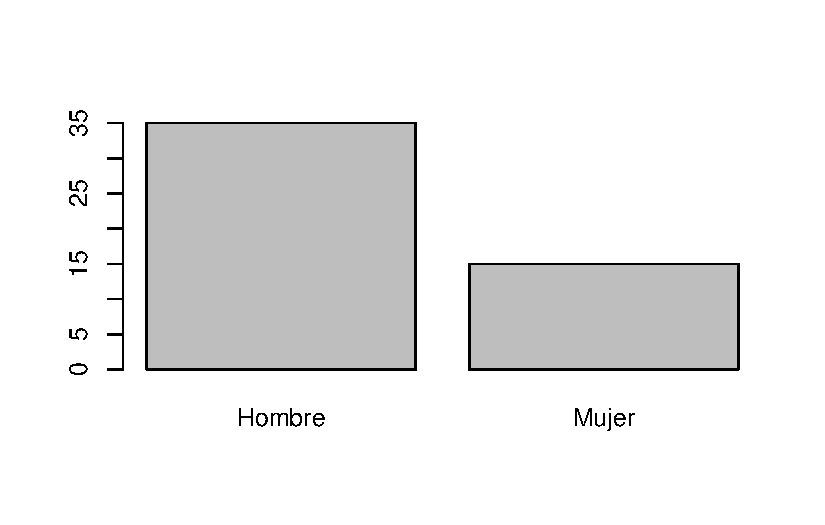
\includegraphics{./PR_1_lect_files/figure-pdf/unnamed-chunk-6-1.pdf}

}

\end{figure}

Los elementos de las listas pueden también tener nombres y ser llamados
por ellos. Esta lista no los tiene, pero se le pueden asignar utilizando
un simple vector (recordad que en R hay muchas estructuras vectoriales).

\begin{Shaded}
\begin{Highlighting}[]
\FunctionTok{names}\NormalTok{(lista1) }\OtherTok{\textless{}{-}} \FunctionTok{c}\NormalTok{(}\StringTok{\textquotesingle{}mi\_vector\textquotesingle{}}\NormalTok{,}\StringTok{\textquotesingle{}mi\_matriz\textquotesingle{}}\NormalTok{,}\StringTok{\textquotesingle{}mi\_dataframe\textquotesingle{}}\NormalTok{,}\StringTok{\textquotesingle{}mi\_gráfico\textquotesingle{}}\NormalTok{)}\CommentTok{\#este vector asigna nombres a los elementos. Ha de ser de la misma longitud que el número de elementos.}
\end{Highlighting}
\end{Shaded}

Ahora podemos usar el nombre para llamar a los elementos de la lista,
parecido a lo que hacíamos para llamar a las variables dentro de un
dataframe.

\begin{Shaded}
\begin{Highlighting}[]
\FunctionTok{head}\NormalTok{(lista1}\SpecialCharTok{$}\NormalTok{mi\_dataframe,}\AttributeTok{n =} \DecValTok{10}\NormalTok{) }\CommentTok{\#Uso head con al argumento n=10 para que solo muestre las 10 primeras filas.}
\end{Highlighting}
\end{Shaded}

\begin{verbatim}
     id pas    sex
1  1001 114 Hombre
2  1002 125 Hombre
3  1003 120  Mujer
4  1004 115  Mujer
5  1005 111 Hombre
6  1006 120  Mujer
7  1007 118 Hombre
8  1008 124 Hombre
9  1009 123 Hombre
10 1010 126  Mujer
\end{verbatim}

\hypertarget{funciones-un-par-de-palabras}{%
\subsubsection{Funciones (un par de
palabras)}\label{funciones-un-par-de-palabras}}

A lo largo de esta sesión, de manera más o menos consciente, habéis
trabajado con funciones. Estas funciones están contenidas en las
librerías que hemos mencionado al inicio de la sesión. Podemos generar
nuestras propias funciones, pero en mi opinión es preferible introducir
su creación en clases más avanzadas.

Aunque es cierto que cuando eres capaz de crear una función entiendes
mejor su funcionamiento, no es necesario saber hacerlo para utilizarlas
correctamente, pero sí es necesario comentar, aunque sea brevemente, su
estructura.

Como hemos comentado, cuando la librería está cargada (recordad que se
cargan con la función library\footnote{Ejecutando en la consola
  \emph{library(library\_name)}}), basta con llamar a la función para
ejecutarla. Como habéis visto, el nombre de la función va seguido de
unos paréntesis que contienen lo que llamamos \emph{``argumentos''}. Los
argumentos nos permiten personalizar la función al objetivo. Cada
argumento tiene un nombre, y en muchos casos un valor por defecto. En el
fondo la forma de llamar (ejecutar) la función se parece
estructuralmente a un vector en el que cada elemento tiene un nombre y
el valor de cada argumento es utilizado para ejecutar la función.

En muchos casos podemos ver el código detras de una función\footnote{Esto
  tiene que ver en parte con la naturaleza abierta del software libre;
  permite que otros desarrolladores puedan mejorar la función o crear
  otra a partir de ella.}. Por ejemplo, este sería el código que ejecuta
la función ls()

\begin{Shaded}
\begin{Highlighting}[]
\NormalTok{ls }\CommentTok{\#Para poder verlo he de ejecutar la función sin argumentos, sin el contenido de los paréntesis.}
\end{Highlighting}
\end{Shaded}

\begin{verbatim}
function (name, pos = -1L, envir = as.environment(pos), all.names = FALSE, 
    pattern, sorted = TRUE) 
{
    if (!missing(name)) {
        pos <- tryCatch(name, error = function(e) e)
        if (inherits(pos, "error")) {
            name <- substitute(name)
            if (!is.character(name)) 
                name <- deparse(name)
            warning(gettextf("%s converted to character string", 
                sQuote(name)), domain = NA)
            pos <- name
        }
    }
    all.names <- .Internal(ls(envir, all.names, sorted))
    if (!missing(pattern)) {
        if ((ll <- length(grep("[", pattern, fixed = TRUE))) && 
            ll != length(grep("]", pattern, fixed = TRUE))) {
            if (pattern == "[") {
                pattern <- "\\["
                warning("replaced regular expression pattern '[' by  '\\\\['")
            }
            else if (length(grep("[^\\\\]\\[<-", pattern))) {
                pattern <- sub("\\[<-", "\\\\\\[<-", pattern)
                warning("replaced '[<-' by '\\\\[<-' in regular expression pattern")
            }
        }
        grep(pattern, all.names, value = TRUE)
    }
    else all.names
}
<bytecode: 0x000001b10cf75928>
<environment: namespace:base>
\end{verbatim}

Al principio el código es ininteligible, pero según vas aprendiendo, y
especialmente cuando diseñas tus propias funciones, es cada vez más
\emph{lógico}, al fin y al cabo se trata de comunicarse con una máquina.

Pero lo que nos interesa es que comprendáis la gramática que esconde una
función. Aquí la ayuda es de gran valor.

\begin{Shaded}
\begin{Highlighting}[]
\NormalTok{ ?ls }\CommentTok{\#Pido ayuda sobre la función, por eso utilizo solo un ?}
\end{Highlighting}
\end{Shaded}

Al ejecutarlo, debería aparecer algo como esto en la pestaña Help del
panel inferior derecho (si no se ha cambiado la configuración
predeterminada):

\begin{figure}

{\centering 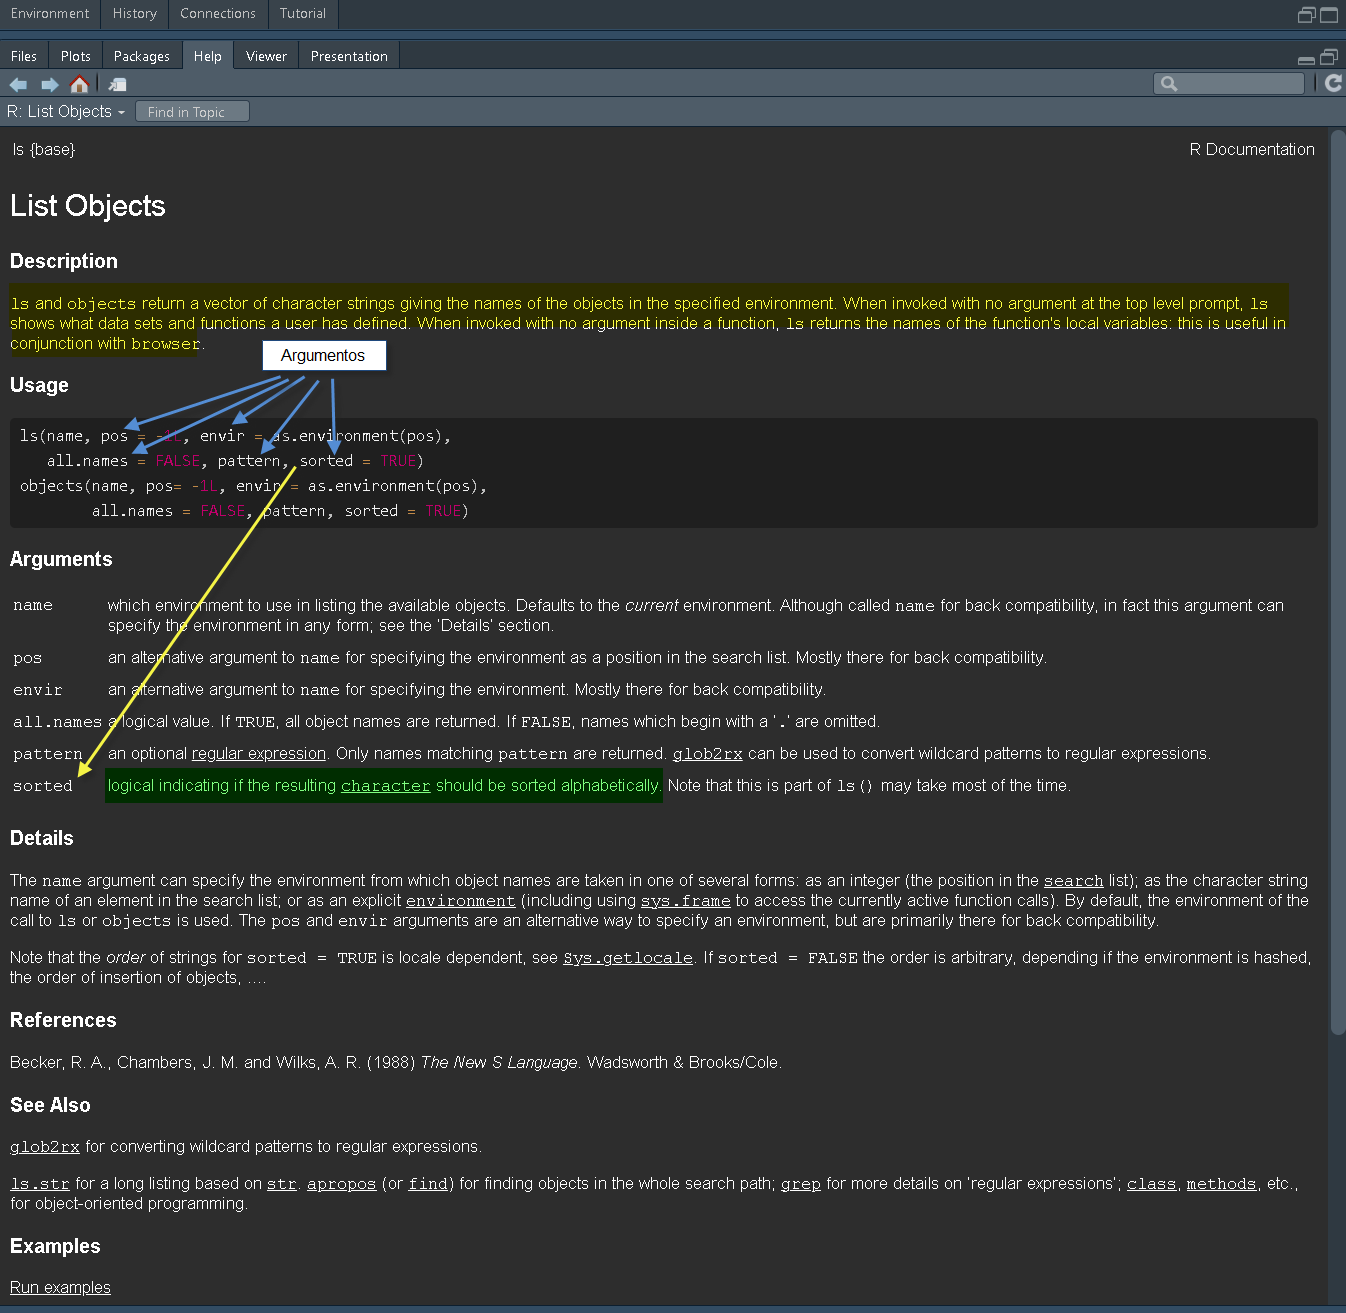
\includegraphics{./pics/ejemplo_ayuda_ls.png}

}

\caption{Ejemplo de ayuda sobre una función}

\end{figure}

El primer bloque, \textbf{Description} describe qué hace la
función\footnote{Como podéis ver, sin comprender algunos conceptos como
  qué es un objeto, qué es un vector o qué es lo que llama environment
  (entorno) es difícil entender la ayuda, de ahí parte de la utilidad de
  enseñar esto antes de enseñar \emph{modern R}}.

Pero me interesa más que entendáis el segundo y tercer bloque
\textbf{Usage} y \textbf{Arguments}. En el bloque \textbf{Usage} podéis
ver una parte de lo que, con permiso de los puristas, llamaría
\emph{gramática de R}. Entre paréntesis, aparecen los nombres de los
argumentos y, a veces, el valor por defecto\footnote{No os fiéis del
  color porque depende del fondo que utilicéis en las opciones de
  RStudio} Cuando no tiene valor por defecto es que no lo necesita
obligatoriamente, pero si lo deseas puedes asignarle un valor para
conseguir que la función opere con dicha especificación. ¿Cualquier
valor? No. El tipo de valor que acoge(a veces es un objeto, como una
matriz, un dataframe, un vector\ldots)se explica en la sección
\textbf{Arguments}.

Lo que viene ahora se explica poco, aunque se usa mucho, con frecuencia
de manera inconsciente. Como os decía, estructuramente se parece mucho a
un vector (en R, muchas estructuras son vectoriales), y como ocurre con
los vectores, las posiciones son relevantes. Cada argumento tiene una
posición reservada. Si la información que necesita el argumento se
coloca en la posición reservada, la función interpreta el valor
\textbf{sin necesidad de que le indiques el nombre del argumento},
porque está \emph{donde se le espera}. Pero no es obligado darle los
argumentos en orden, los puedes cambiar de lugar; eso sí, si los cambias
de lugar, deberás indicarle a qué argumento te refieres, porque \emph{ya
no está donde se le esperaba}.

Por ejemplo:

El argumento \emph{sorted} está en la posición 5. Es un argumento lógico
(TRUE/FALSE) que sirve pare decirle que ordene el resultado de la orden
listar los objetos del espacio de trabajo.

Si lo coloco en la posición en la que lo espera\ldots{}

\begin{Shaded}
\begin{Highlighting}[]
\FunctionTok{ls}\NormalTok{(,,,,,}\ConstantTok{TRUE}\NormalTok{)}
\end{Highlighting}
\end{Shaded}

\begin{verbatim}
 [1] "a1"         "a2"         "a2.1"       "a3"         "Anscombe"  
 [6] "ar"         "ar2"        "b"          "d"          "df1"       
[11] "iris"       "lista1"     "m1"         "m2"         "p1"        
[16] "v1"         "vecnam.rep" "x"          "y"         
\end{verbatim}

\ldots{} ordena por orden alfabético la lista de los objetos que hemos
ido generando.

Lo mismo sucede si le hubiéramos indicado el nombre del argumento.

\begin{Shaded}
\begin{Highlighting}[]
\FunctionTok{ls}\NormalTok{(}\AttributeTok{sorted=}\ConstantTok{TRUE}\NormalTok{)}
\end{Highlighting}
\end{Shaded}

\begin{verbatim}
 [1] "a1"         "a2"         "a2.1"       "a3"         "Anscombe"  
 [6] "ar"         "ar2"        "b"          "d"          "df1"       
[11] "iris"       "lista1"     "m1"         "m2"         "p1"        
[16] "v1"         "vecnam.rep" "x"          "y"         
\end{verbatim}

Pero si le indico el valor del argumento sin el nombre del mismo, o sin
colocarlo en la posición adecuada, sucede esto:

\begin{Shaded}
\begin{Highlighting}[]
\FunctionTok{ls}\NormalTok{(}\ConstantTok{TRUE}\NormalTok{)}
\end{Highlighting}
\end{Shaded}

La función cree que el valor TRUE es para el argumento name, que no es
un argumento de tipo lógico (TRUE/FALSE).

\emph{Todas las funciones de R funcionan así}. Es raro que necesitemos
utilizar todos los argumentos, por lo que en general acabaremos
indicando el nombre y el valor solo de los argumentos necesarios para
que la función haga lo que nosotros deseamos, sin embargo es frecuente
encontrarse en los blogs de consulta, código en el que no se indica el
argumento. Esta es la explicación.

Para terminar este apartado sobre objetos, solo queda decir que hay
muchos otros tipos de objetos, algunas funciones crean sus propios
objetos, aunque con frecuencia contienen uno o más de los que hemos
visto.

En la siguiente sesión veremos cómo importar datos para construir un
dataframe y trasnformarlo para obtener nuevas variables.

\bookmarksetup{startatroot}

\hypertarget{pr2-importaciuxf3n-de-datos.}{%
\chapter{PR2-Importación de datos.}\label{pr2-importaciuxf3n-de-datos.}}

Recuerda siempre cómo \emph{``piensa''} R.

\begin{figure}

{\centering 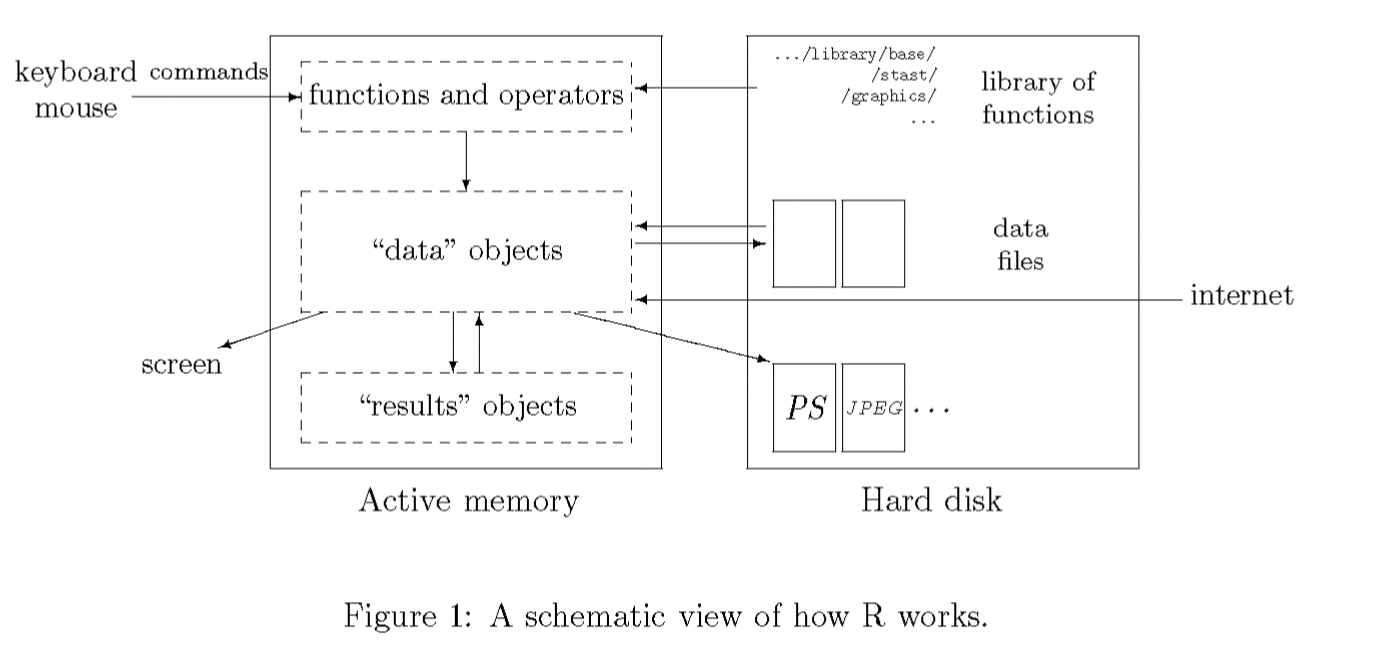
\includegraphics[width=0.75\textwidth,height=\textheight]{./pics/como_piensa_R.png}

}

\caption{Cómo piensa R}

\end{figure}

En la sección anterior hemos visto lo fundamental sobre estructuras y
hemos comentado las características de una estructura clave en el manejo
de datos en R: \textbf{dataframe}.

En esta práctica vamos a ver cómo importar datos utilizando diferentes
funciones dependiendo del origen.

Como comentábamos, la importación consiste en construir un objeto,
generalmente de tipo dataframe a partir de un archivo externo.

Para hacerlo necesitamos que el archivo externo tenga una estructura
matricial (.xlsx) o que pueda convertirse en matricial (.csv) porque
incluya caracteres de separación que le indiquen al programa que lo
importa, en nuestro caso R, cuando cambiamos de columna o de fila.

Se han incorporado muchas funciones a R que realizan la importación de
forma casi automática, pero entender sus fundamentos puede ayudar a
entender y resolver problemas de importación.

Nos vamos a centrar en dos estructuras desde las que con frecuencia
vamos a importar datos.

\hypertarget{importaciuxf3n-desde-archivo-.csv-comma-separated-values.}{%
\subsection{Importación desde archivo .csv (Comma Separated
Values).}\label{importaciuxf3n-desde-archivo-.csv-comma-separated-values.}}

Una de las más sencillas si el archivo .csv está bien construido. Un
archivo .csv no es más que un archivo de texto en el que el carácter
coma (``,'') separa campos (variables) y el salgo de línea separa
registros (individuos/elementos).

\begin{quote}
En realidad cualquier estructura de texto que utilice un separador de
campos (variables) y de registros (líneas) es susceptible de ser
importada. R tiene una función muy básica para hacerlo
(\emph{read.table}), a la que le indicamos el carácter separador de
campos (``,'', ``;'',``/'',``/tab''\ldots), si el archivo contiene
encabezado (header), una primera línea en la que se almacenan los
nombres de las variables, o el carácter que utiliza como separador
decimal. En realidad tiene muchos otros argumentos, pero no son
necesarios para realizar importaciones sencillas. Por ejemplo, la
función que utilizaremos a continuación en realida es una adaptación de
esta en la que por defecto se establece que el separador de campos es la
coma (``,''), entre otros argumentos.
\end{quote}

Como comentábamos, el .csv es un formato estándar, que pesa poco y hay
funciones diseñadas para leer este tipo de archivos.

Entre los archivos de trabajo, hemos incluido un archivo llamado myiam2.
Es un archivo con extensión .csv que contiene una base de datos de
pacientes que habían padecido un infarto.

Vamos a crear un dataframe importándola y como sabemos que se trata de
un csv, vamos a utilizar al función \emph{read.csv} del paquete
\emph{utils}. En este caso no hace falta cargarla porque este paquete se
carga al iniciar R.

Recuerde que hay que indicar el dirección en la que está el archivo. En
este ejemplo, que explicaremos en clase, vamos a utilizar
direccionamiento relativo al directorio en el que está el archivo desde
mi directorio de trabajo.

\begin{quote}
Importante. La dirección de las barras de dirección (las que separan
directorios y subdirectorios) en R vienen del mundo UNIX (un sistema
operativo diferente a Windows), por eso las barras se inclinan hacia el
lado contrario. En clase veremos alguna función que facilita copiar y
pegar las direcciones desde Windows adaptándolas al lenguaje de R. Se
puede hacer invirtiendo las barras que vienen de Windows, o
duplicándolas manteniendo la dirección.
\end{quote}

\begin{Shaded}
\begin{Highlighting}[]
\NormalTok{iam}\OtherTok{\textless{}{-}}\FunctionTok{read.csv}\NormalTok{(}\StringTok{\textquotesingle{}\_data/myiam2.csv\textquotesingle{}}\NormalTok{) }\CommentTok{\# Utilizando relative path.}
\end{Highlighting}
\end{Shaded}

La salidas de las funciones read suele ser un dataframe, y por ello
podemos asignarlo directamente a un objeto, en el ejemplo el objeto
(dataframe) llamado iam.

Pedimos las primeras filas del dataframe.

\begin{Shaded}
\begin{Highlighting}[]
\FunctionTok{head}\NormalTok{(iam)}
\end{Highlighting}
\end{Shaded}

\begin{verbatim}
  Id      Age Sex Height Weight Smoke ami
1  1 65.24100   1   1.62  74.56     0   0
2  2 62.45461   0   1.56  60.89     0   0
3  3 64.68328   0   1.69  74.20     0   0
4  4 65.36045   0   1.34  43.92     0   0
5  5 70.71094   0   1.81  80.86     1   0
6  6 65.42030   0   1.78  80.56     0   0
\end{verbatim}

También podemos pedir la estructura que nos da mucha información sobre
el contenido del dataframe.

\begin{Shaded}
\begin{Highlighting}[]
\FunctionTok{str}\NormalTok{(iam)}
\end{Highlighting}
\end{Shaded}

\begin{verbatim}
'data.frame':   100 obs. of  7 variables:
 $ Id    : int  1 2 3 4 5 6 7 8 9 10 ...
 $ Age   : num  65.2 62.5 64.7 65.4 70.7 ...
 $ Sex   : int  1 0 0 0 0 0 1 0 0 0 ...
 $ Height: num  1.62 1.56 1.69 1.34 1.81 1.78 1.79 1.44 1.56 1.87 ...
 $ Weight: num  74.6 60.9 74.2 43.9 80.9 ...
 $ Smoke : int  0 0 0 0 1 0 0 1 0 0 ...
 $ ami   : int  0 0 0 0 0 0 0 1 0 0 ...
\end{verbatim}

En realidad esta estructura también está visible si desplegamos el
dataframe en la pestaña Environment, ventana data del panel superior
derecho.

\begin{figure}

{\centering 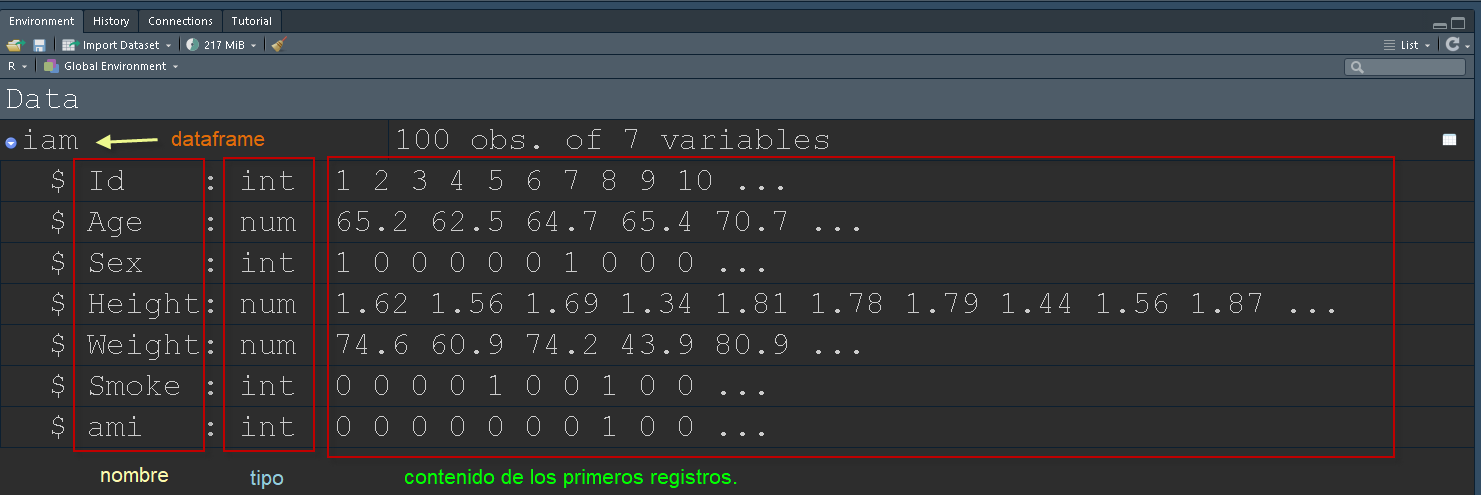
\includegraphics{./pics/iam_en_vent_data.png}

}

\caption{vent\_data}

\end{figure}

Esta función nos informa del contenido del objeto. Al tratarse de un
dataframe, nos muestra las variables, el tipo de dato que almacena cada
una (en este ejemplo solo hay numérico y enteros) y las primeras
observaciones. Es el primer punto de control en el que podemos observar
si la importación ha ido como esperábamos.

\hypertarget{importaciuxf3n-desde-archivo-.xlsx-excel.}{%
\subsection{Importación desde archivo .xlsx
(Excel).}\label{importaciuxf3n-desde-archivo-.xlsx-excel.}}

El concepto de importación es el mismo independientemente de la fuente
de los datos, pero las funciones a utilizar cambian para responder a las
especificidades del tipo de archivo.

R no cuenta con función propia para leer un archivo xlsx, pero otras
librerías lo han incorporado.

El siguiente ejemplo crea el mismo dataframe, pero en esta ocasión desde
un archivo .xlsx. Utilizaremos la librería \emph{readxl} (si no la tiene
instalada, hágalo antes de ejecutar el siguiente código).

Podríamos cargar la librería con library(readxl), pero vamos a
aprovechar para mostrar cómo podemos llamar a una biblioteca (library)
sin cargarla en memoria. La clave es anteceder el nombre de la función
con el nombre de la biblioteca seguido de \emph{``::''}.

\begin{Shaded}
\begin{Highlighting}[]
\NormalTok{iam2}\OtherTok{\textless{}{-}}\NormalTok{readxl}\SpecialCharTok{::}\FunctionTok{read\_xlsx}\NormalTok{(}\StringTok{\textquotesingle{}\_data/myiam3.xlsx\textquotesingle{}}\NormalTok{)}
\end{Highlighting}
\end{Shaded}

Pedimos la estructura

\begin{Shaded}
\begin{Highlighting}[]
\FunctionTok{str}\NormalTok{(iam2)}
\end{Highlighting}
\end{Shaded}

\begin{verbatim}
tibble [100 x 8] (S3: tbl_df/tbl/data.frame)
 $ Id    : num [1:100] 1 2 3 4 5 6 7 8 9 10 ...
 $ Sex   : chr [1:100] "1" "0" "0" "0" ...
 $ Height: num [1:100] 1.62 1.56 1.69 1.34 1.81 1.78 1.79 1.44 1.56 1.87 ...
 $ Weight: num [1:100] 74.6 60.9 74.2 43.9 80.9 ...
 $ Smoke : chr [1:100] "0" "0" "0" "0" ...
 $ Ami   : chr [1:100] "0" "0" "0" "0" ...
 $ fecing: POSIXct[1:100], format: "2015-03-18 21:05:08" "2015-08-07 04:23:18" ...
 $ fnac  : POSIXct[1:100], format: "1949-12-20 14:28:28" "1953-02-21 15:15:57" ...
\end{verbatim}

En realidad vemos que la nueva base de datos no es exactamente la
anterior. Las variables Sex, Smoke y Ami son de tipo carácter. Además no
incluye la edad, pero sí la fecha de ingreso y la fecha de nacimiento.

No es infrecuente que nuestros datos procedan de otro paquete
estadístico o tipo de fichero. La biblioteca \emph{foreign} incluye
funciones para acometer esta tarea desde varias fuentes, incluyendo los
tres software de análisis más habituales en nuestro contexto
(SAS,SPSS,Stata).

\begin{longtable}[]{@{}
  >{\raggedright\arraybackslash}p{(\columnwidth - 6\tabcolsep) * \real{0.0658}}
  >{\raggedright\arraybackslash}p{(\columnwidth - 6\tabcolsep) * \real{0.0700}}
  >{\raggedright\arraybackslash}p{(\columnwidth - 6\tabcolsep) * \real{0.0700}}
  >{\raggedright\arraybackslash}p{(\columnwidth - 6\tabcolsep) * \real{0.7860}}@{}}
\toprule()
\begin{minipage}[b]{\linewidth}\raggedright
~~~\\
\textbf{Programa}\\
\hspace*{0.333em}\hspace*{0.333em}\hspace*{0.333em}\\
\strut
\end{minipage} & \begin{minipage}[b]{\linewidth}\raggedright
~~~\\
\textbf{Paquete}\strut
\end{minipage} & \begin{minipage}[b]{\linewidth}\raggedright
~~~\\
\textbf{Función}\strut
\end{minipage} & \begin{minipage}[b]{\linewidth}\raggedright
~~~\\
\textbf{Argumentos y opciones más~~~frecuentes/predefinidas}\strut
\end{minipage} \\
\midrule()
\endhead
\begin{minipage}[t]{\linewidth}\raggedright
~~~\\
SPSS\strut
\end{minipage} & \begin{minipage}[t]{\linewidth}\raggedright
~~~\\
foreign\strut
\end{minipage} & \begin{minipage}[t]{\linewidth}\raggedright
~~~\\
read.spss()\strut
\end{minipage} & \begin{minipage}[t]{\linewidth}\raggedright
~~~\\
read.spss(file,~~~use.value.labels = TRUE,~~~to.data.frame = FALSE,
max.value.labels = Inf, trim.factor.names = FALSE,~~~trim\_values =
TRUE, reencode = NA, use.missings = to.data.frame)\strut
\end{minipage} \\
\begin{minipage}[t]{\linewidth}\raggedright
~~~\\
Stata\strut
\end{minipage} & \begin{minipage}[t]{\linewidth}\raggedright
~~~\\
foreign\strut
\end{minipage} & \begin{minipage}[t]{\linewidth}\raggedright
~~~\\
read.dta()\strut
\end{minipage} & \begin{minipage}[t]{\linewidth}\raggedright
~~~\\
read.dta(file, convert.dates = TRUE,~~~convert.factors = TRUE,
missing.type = FALSE, convert.underscore = FALSE,~~~warn.missing.labels
= TRUE)\strut
\end{minipage} \\
\begin{minipage}[t]{\linewidth}\raggedright
~~~\\
SAS\strut
\end{minipage} & \begin{minipage}[t]{\linewidth}\raggedright
~~~\\
haven\strut
\end{minipage} & \begin{minipage}[t]{\linewidth}\raggedright
~~~\\
read\_sas()\strut
\end{minipage} & \begin{minipage}[t]{\linewidth}\raggedright
~~~\\
read\_sas(data\_file,~~~catalog\_file = NULL, encoding = NULL,
cols\_only = NULL)\strut
\end{minipage} \\
\bottomrule()
\end{longtable}

También existen paquetes más específicos para importar desde alguno de
ellos, como \emph{readstata13}, que permiten opciones adicionales.

\hypertarget{guardar-los-datos-para-la-siguiente-sesiuxf3n.}{%
\section{Guardar los datos para la siguiente
sesión.}\label{guardar-los-datos-para-la-siguiente-sesiuxf3n.}}

Una vez hemos trabajado los datos en R, no tendría mucho sentido volver
a exportarlos con las nuevas variables creadas, salvo que deseemos
enviárselo a alguien que no utilice R o no pueda importar su formato de
datos.

Podríamos guardar toda la imagen del espacio de trabajo (Workspace) y
cargarla antes de trabajar con el nuevo dataframe en la siguiente
sesión.

Sin embargo, y aunque cueste entenderlo al principio, es preferible
guadar la menor cantidad de objetos posibles y tratar de que sea el
código el que lo construya cada vez.

Si el objeto es muy grande o lleva mucho tiempo volver a generarlo con
código, puede estar justificado guardar el o los objetos concretos.

En el caso del dataframe tenemos una estructura de datos que le sirve a
R para gestionar esta parte. Son los archivos .RDS.

En este vínculo explican las dos opciones, pero de momento prefiero
utilizar un archivo .RDS. Solo necesita un par de argumentos, el nombre
del objeto dataframe que queremos guardar y el nombre del archivo en el
que queremos guardarlo.

El dataframe que nos interesa es iam, porque contiene las nuevas
variables y las transformaciones que hemos realizado. Incluyo los
nombres de los argumentos, pero dado que son los dos primeros en
realidad no haría falta\footnote{Recordad que siempre es mejor utilizar
  direccionamiento relativo (/\_data/iam.RDS) en vez de absoluto
  (`C:/Users/Usuario/Documents/SUB1/SUB2/SUB3/SUB4/SUB5/SUB6/dataiam.RDS')
  - atención a la dirección de la barra si copiasteis el path desde
  Windows}.

\begin{Shaded}
\begin{Highlighting}[]
\FunctionTok{saveRDS}\NormalTok{(}\AttributeTok{object=}\NormalTok{iam,}\AttributeTok{file=}\StringTok{\textquotesingle{}iam.RDS\textquotesingle{}}\NormalTok{)}
\end{Highlighting}
\end{Shaded}

Es importante que aprendáis a salvarlo (ahora y tras el capítulo de
manipulación de datos), porque lo utilizaremos en futuras sesiones.

\bookmarksetup{startatroot}

\hypertarget{pr3-manipulaciuxf3n-de-datos.}{%
\chapter{PR3-Manipulación de
datos.}\label{pr3-manipulaciuxf3n-de-datos.}}

Recuerda siempre cómo \emph{``piensa''} R.

\begin{figure}

{\centering 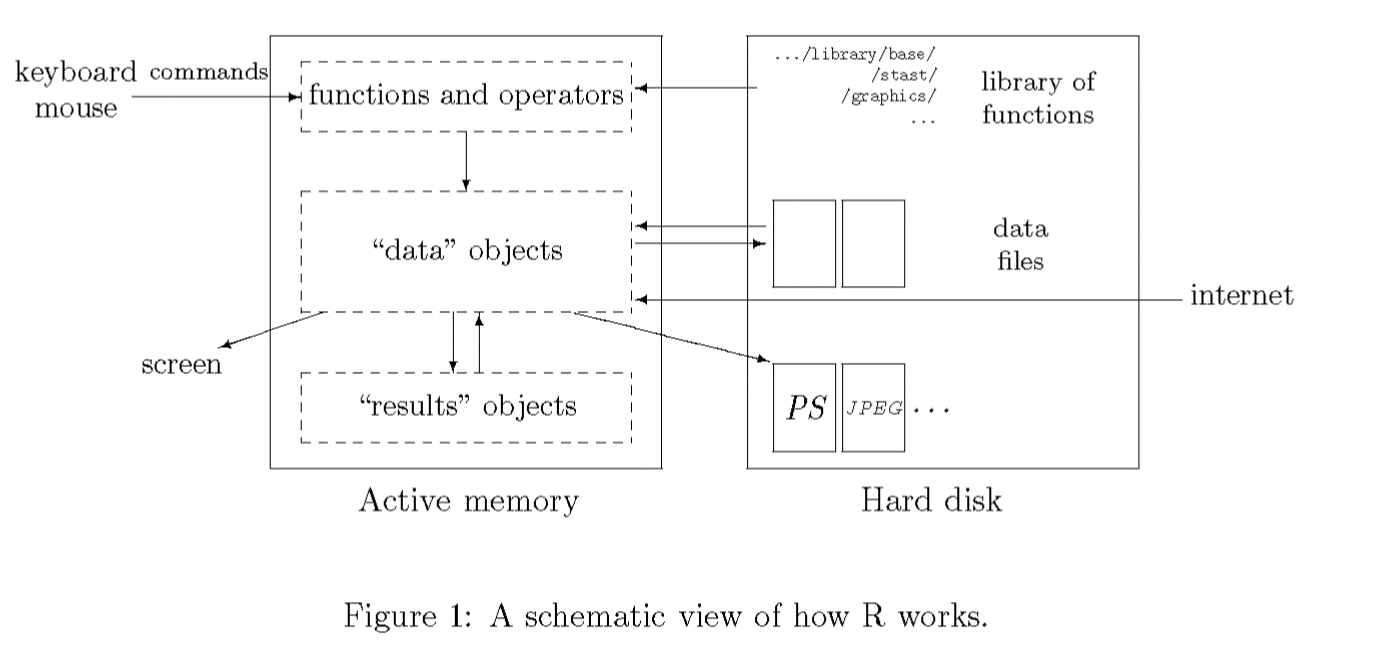
\includegraphics[width=0.75\textwidth,height=\textheight]{./pics/como_piensa_R.png}

}

\caption{Cómo piensa R}

\end{figure}

En la sección anterior hemos visto cómo importar datos y como
transformarlos usando \emph{base R}.

Si tienes problemas con la importación, echa un vistazo a las notas de
la sesión anterior.

En esta sesión aprenderemos a manipular los datos para, por ejemplo,
construir nuevas variables a partir de las originales. Lo haremos
utilizando \emph{base R}, pero también incluiremos al final cómo hacer
lo mismo con \emph{modern R}.

\hypertarget{importaciuxf3n-de-datos.}{%
\section{Importación de datos.}\label{importaciuxf3n-de-datos.}}

Antes de hablar de transformaciones, vamos a repasar las funciones que
utilizamos para construir el dataframe.

\begin{Shaded}
\begin{Highlighting}[]
\NormalTok{iam}\OtherTok{\textless{}{-}}\FunctionTok{read.csv}\NormalTok{(}\StringTok{\textquotesingle{}\_data/myiam2.csv\textquotesingle{}}\NormalTok{) }\CommentTok{\# Utilizando relative path.}
\end{Highlighting}
\end{Shaded}

Recuerde que la salidas de las funciones ``read'' suelen ser dataframes,
y por ello podemos asignarlo directamente a un objeto, en el ejemplo el
objeto (dataframe) llamado iam.

Primeras filas del dataframe.

\begin{Shaded}
\begin{Highlighting}[]
\FunctionTok{head}\NormalTok{(iam)}
\end{Highlighting}
\end{Shaded}

\begin{verbatim}
  Id      Age Sex Height Weight Smoke ami
1  1 65.24100   1   1.62  74.56     0   0
2  2 62.45461   0   1.56  60.89     0   0
3  3 64.68328   0   1.69  74.20     0   0
4  4 65.36045   0   1.34  43.92     0   0
5  5 70.71094   0   1.81  80.86     1   0
6  6 65.42030   0   1.78  80.56     0   0
\end{verbatim}

Estructura del dataframe (en realidad la puedes ver en la pestaña
Environment del panel superior derecho {[}en esta configuración{]})

\begin{Shaded}
\begin{Highlighting}[]
\FunctionTok{str}\NormalTok{(iam)}
\end{Highlighting}
\end{Shaded}

\begin{verbatim}
'data.frame':   100 obs. of  7 variables:
 $ Id    : int  1 2 3 4 5 6 7 8 9 10 ...
 $ Age   : num  65.2 62.5 64.7 65.4 70.7 ...
 $ Sex   : int  1 0 0 0 0 0 1 0 0 0 ...
 $ Height: num  1.62 1.56 1.69 1.34 1.81 1.78 1.79 1.44 1.56 1.87 ...
 $ Weight: num  74.6 60.9 74.2 43.9 80.9 ...
 $ Smoke : int  0 0 0 0 1 0 0 1 0 0 ...
 $ ami   : int  0 0 0 0 0 0 0 1 0 0 ...
\end{verbatim}

Recuerde que esta estructura también está visible si desplegamos el
dataframe en la pestaña Environment, ventana data del panel superior
derecho.

\begin{figure}

{\centering 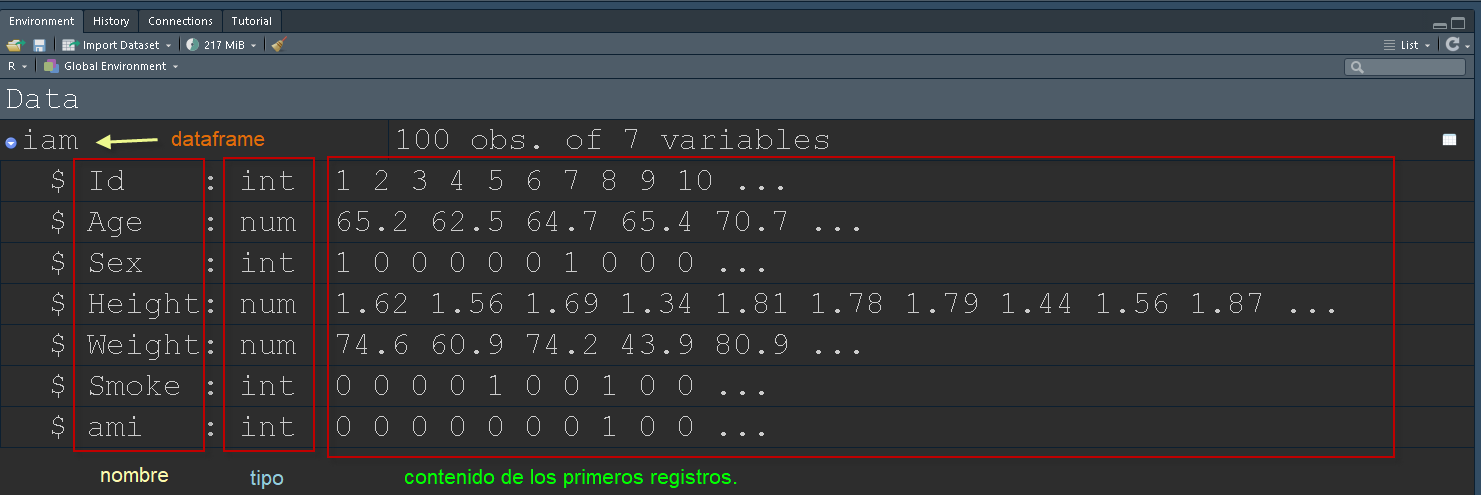
\includegraphics{./pics/iam_en_vent_data.png}

}

\caption{vent\_data}

\end{figure}

\hypertarget{manipulaciuxf3n-de-datos.}{%
\section{Manipulación de datos.}\label{manipulaciuxf3n-de-datos.}}

Antes de poder modificar variables existentes o crear algunas nuevas,
necesitamos conocer algunas funciones y operadores básicos incluidos en
la instalación básica de r.

\hypertarget{operadores.}{%
\subsection{Operadores.}\label{operadores.}}

\begin{longtable}[]{@{}cc@{}}
\toprule()
Operadores comparativos & Símbolo/instrucción \\
\midrule()
\endhead
igualdad & == \\
desigualdad & != \\
menor & \textless{} \\
menor igual & \textless= \\
mayor & \textgreater{} \\
maryor igual & \textgreater= \\
\bottomrule()
\end{longtable}

\begin{longtable}[]{@{}cc@{}}
\toprule()
Operadores lógicos & Símbolo/instrucción \\
\midrule()
\endhead
AND lógica & \& \\
OR lógica & \textbar{} \\
negación lógica & ! \\
Identidad & \&\& \\
\bottomrule()
\end{longtable}

\hypertarget{funciones-buxe1sicas.}{%
\subsection{Funciones básicas.}\label{funciones-buxe1sicas.}}

\begin{longtable}[]{@{}cc@{}}
\toprule()
\textbf{Operador/Función} & \textbf{Símbolo/instrucción} \\
\midrule()
\endhead
suma & + \\
resta & - \\
multiplicación & * \\
división & / \\
módulo & \%\% (resto de división) \\
división entera & \%/\% \\
raíz cuadrada & sqrt \\
logaritmo natural (base e) & log \\
logaritmos genérico (base-\textgreater b) & logb (ex. log10(45)) \\
número e elevado a x & exp(x) \\
máximo & max \\
mínimo & min \\
rango & range \\
longitud & length \\
sumatorio & sum \\
productorio & prod \\
media & mean \\
mediana & median \\
desv. estándar & sd \\
varianza & var \\
\bottomrule()
\end{longtable}

\hypertarget{manipulaciones-muxe1s-frecuentes.}{%
\subsection{Manipulaciones más
frecuentes.}\label{manipulaciones-muxe1s-frecuentes.}}

Seguiremos utilizando el dataframe generado anteriormente llamado
\emph{iam}.

\hypertarget{recodificar-en-base-a-puntos-de-corte.-convertir-numuxe9rica-en-factor}{%
\subsubsection{Recodificar en base a puntos de corte. (Convertir
numérica en
factor)}\label{recodificar-en-base-a-puntos-de-corte.-convertir-numuxe9rica-en-factor}}

La función cut es muy útila para generar una variable categórica a
partir de una cuantitativa discreta o continua. Solo necesitas que le
entregemos el vector a cortar y los puntos de corte. Veamos un par de
ejemplos.

Construiremos grupos de edad e intervalos de 10 años. El máximo de esta
variable es 70.71 y el mínimo es 59.5, así pues nos hacen falta puntos
de corte entre ambos valores con amplitud de 10 años.

\begin{Shaded}
\begin{Highlighting}[]
\NormalTok{iam}\SpecialCharTok{$}\NormalTok{age5}\OtherTok{\textless{}{-}}\FunctionTok{cut}\NormalTok{(iam}\SpecialCharTok{$}\NormalTok{Age,}\FunctionTok{seq}\NormalTok{(}\DecValTok{55}\NormalTok{,}\DecValTok{75}\NormalTok{,}\DecValTok{10}\NormalTok{),}\AttributeTok{include.lowest =}\NormalTok{ T,}\AttributeTok{right =}\NormalTok{ T) }\CommentTok{\# la función seq nos facilita la tarea de construir el vector de puntos de corte.}
\end{Highlighting}
\end{Shaded}

La propia función genera un factor (ya hablaremos de este tipo de
objetos que servirán para almacenar variables categóricas )

Podemos construir una tabla para comprobar la distribución de la nueva
variable categórica.

\begin{Shaded}
\begin{Highlighting}[]
\FunctionTok{table}\NormalTok{(iam}\SpecialCharTok{$}\NormalTok{age5)}
\end{Highlighting}
\end{Shaded}

\begin{verbatim}

[55,65] (65,75] 
     47      53 
\end{verbatim}

Como se puede observar, la propia función genera las etiquetas de los
intervalos en función de los puntos de corte que le hemos dado. A tener
en cuenta:

\begin{verbatim}
* La función *cut* tiene argumentos para poder construir los intervalos cerrando el intervalo por su límite derecho (argumento right=T) .
* la función *cut* genera un objeto de tipo vector y de clase factor, por lo que sus etiquetas de nivel se pueden modificar (lo veremos al hablar de factores).
* la función *cut* puede cerrar el intervalo inferior (argumento include.lowest=T)
\end{verbatim}

\hypertarget{construir-variables-operando-otras.}{%
\subsubsection{Construir variables operando
otras.}\label{construir-variables-operando-otras.}}

En el dataframe \emph{iam} se incluyen las variables peso y altura.
Vamos a construir el Índice de Masa Corporal.

\[IMC=\frac{Peso (kg)}{Altura(m)^2}\]

\begin{Shaded}
\begin{Highlighting}[]
\NormalTok{iam}\SpecialCharTok{$}\NormalTok{bmi}\OtherTok{\textless{}{-}}\NormalTok{iam}\SpecialCharTok{$}\NormalTok{Weight}\SpecialCharTok{/}\NormalTok{iam}\SpecialCharTok{$}\NormalTok{Height}\SpecialCharTok{\^{}}\DecValTok{2}
\end{Highlighting}
\end{Shaded}

Como se puede observar, para incluirla en el dataframe, hemos de
indicárselo utilizando el nombre del mismo seguido de \$ y el nombre que
queremos dar a la nueva variable, en este caso \emph{bmi}.

\hypertarget{recodificaciuxf3n.}{%
\subsubsection{Recodificación.}\label{recodificaciuxf3n.}}

Posiblemente una de las tareas más frecuentes, si no la más frecuente,
manipulando datos es la recodificación, construir una variable
categórica agrupando categorías de otra.

Para entender esta tarea en R, es útil entender la clase factor, la
clase en la que vamos a almacenar las variables categóricas.

\hypertarget{factores-quuxe9-es-un-factor-en-r}{%
\subsubsection{Factores ¿Qué es un factor en
R?}\label{factores-quuxe9-es-un-factor-en-r}}

Los factores son posiblemente uno de los elementos básicos en R que más
cuesta entender. En mi opinión tiene que ver con la confusión entre el
concepto de nivel (level) y la etiqueta (label) que se le asigna a cada
uno de los niveles.

Para explicar cómo funciona, vamos a crear un ejemplo sencillo para ver
cómo operan estas dos características.

Aunque parezca extraño, vamos a partir de un vector de tipo
\emph{integer} para posteriormente convertirlo en uno de tipo factor al
que añadiremos las etiquetas.

\begin{itemize}
\tightlist
\item
  Construcción de un vector numérico.
\end{itemize}

\begin{Shaded}
\begin{Highlighting}[]
\NormalTok{x}\OtherTok{\textless{}{-}}\FunctionTok{rep}\NormalTok{(}\DecValTok{0}\SpecialCharTok{:}\DecValTok{1}\NormalTok{,}\DecValTok{25}\NormalTok{)}
\end{Highlighting}
\end{Shaded}

\begin{itemize}
\tightlist
\item
  Conversión del vector en un factor, sin decirle nada más.
\end{itemize}

\begin{Shaded}
\begin{Highlighting}[]
\NormalTok{sex}\OtherTok{\textless{}{-}}\FunctionTok{factor}\NormalTok{(x)}
\end{Highlighting}
\end{Shaded}

\begin{itemize}
\item
  Al utilizar la función factor, R lee el vector que recibe y, si no le
  decimos otra cosa, identifica los valores diferentes y los ordena en
  orden alfanumérico.
\item
  Acto seguido va asignado el nivel correspondiente a cada valor
  diferente, y utiliza el valor original para construir una etiqueta.
\item
  Lo que obtenemos es un vector de tipo factor que tiene niveles que van
  del 1 al número de valores diferentes que trajese la variable (el
  vector) original. Pero estos niveles están ocultos detrás de las
  etiquetas que se les asignan.
\item
  Lo importante es el nivel, pero su relación con la etiqueta asignada
  nos va a permitir recodificar variables utilizando las etiquetas que
  se les asignan.
\end{itemize}

Veamos un ejemplo.

El vector sex, creado con el código anterior, tiene dos niveles, 1 y 2,
pero las etiquetas que fueron asignadas como indiqué, son ``0'' y ``1'',
valores originales del vector. Al no decirle lo contrario, usó el orden
alfanumérico, por eso el 0 se asigna al primer nivel y el 1 al segundo
nivel.

Si queremos ver los auténticos niveles que contiens podemos forzar una
conversión de tipo de la siguiente manera:

\begin{Shaded}
\begin{Highlighting}[]
\NormalTok{sex}
\end{Highlighting}
\end{Shaded}

\begin{verbatim}
 [1] 0 1 0 1 0 1 0 1 0 1 0 1 0 1 0 1 0 1 0 1 0 1 0 1 0 1 0 1 0 1 0 1 0 1 0 1 0 1
[39] 0 1 0 1 0 1 0 1 0 1 0 1
Levels: 0 1
\end{verbatim}

\begin{Shaded}
\begin{Highlighting}[]
\FunctionTok{as.numeric}\NormalTok{(sex)}
\end{Highlighting}
\end{Shaded}

\begin{verbatim}
 [1] 1 2 1 2 1 2 1 2 1 2 1 2 1 2 1 2 1 2 1 2 1 2 1 2 1 2 1 2 1 2 1 2 1 2 1 2 1 2
[39] 1 2 1 2 1 2 1 2 1 2 1 2
\end{verbatim}

Observe como el primer vector muestra las etiquetas, mientras que el
segundo muestra los niveles.

En realidad podríamos haber impuesto nuestras etiquetas a dichos niveles
en la propia creación del factor, pero para eso debemos entender que si
no le decimos lo contrario, la identificación del orden de asignación
sigue dependiendo del orden alfanumérico.

Para indicarle las etiquetas, basta con meter un vector con las
etiquetas en el argumento \emph{labels.}

En este ejemplo asumimos que el 0 es el valor con el que en la base de
datos original se codificó Hombre y 1 el valor con el que se codificó
Mujer.

\begin{Shaded}
\begin{Highlighting}[]
\NormalTok{sex2}\OtherTok{\textless{}{-}}\FunctionTok{factor}\NormalTok{(x,}\AttributeTok{labels =} \FunctionTok{c}\NormalTok{(}\StringTok{\textquotesingle{}Hombre\textquotesingle{}}\NormalTok{,}\StringTok{\textquotesingle{}Mujer\textquotesingle{}}\NormalTok{))}
\end{Highlighting}
\end{Shaded}

\begin{Shaded}
\begin{Highlighting}[]
\NormalTok{sex2}
\end{Highlighting}
\end{Shaded}

\begin{verbatim}
 [1] Hombre Mujer  Hombre Mujer  Hombre Mujer  Hombre Mujer  Hombre Mujer 
[11] Hombre Mujer  Hombre Mujer  Hombre Mujer  Hombre Mujer  Hombre Mujer 
[21] Hombre Mujer  Hombre Mujer  Hombre Mujer  Hombre Mujer  Hombre Mujer 
[31] Hombre Mujer  Hombre Mujer  Hombre Mujer  Hombre Mujer  Hombre Mujer 
[41] Hombre Mujer  Hombre Mujer  Hombre Mujer  Hombre Mujer  Hombre Mujer 
Levels: Hombre Mujer
\end{verbatim}

\begin{Shaded}
\begin{Highlighting}[]
\FunctionTok{as.numeric}\NormalTok{(sex2)}
\end{Highlighting}
\end{Shaded}

\begin{verbatim}
 [1] 1 2 1 2 1 2 1 2 1 2 1 2 1 2 1 2 1 2 1 2 1 2 1 2 1 2 1 2 1 2 1 2 1 2 1 2 1 2
[39] 1 2 1 2 1 2 1 2 1 2 1 2
\end{verbatim}

Como se puede observar, los niveles (1 y 2) siguen siendo los mismos,
pero las etiquetas han cambiado.

También se obseva como cuando pedimos un vector de clase factor, debajo
aparecen los niveles (Levels: Hombre Mujer) en el orden en que se
asignan a los niveles subyacentes (1 y 2).

Imaginemos que por alguna razón hubiésemos querido que el primer nivel
se asignase a Mujer aunque el código que se asignó en la base de datos
original fue el superior (1). Podemos obligar a que la función lea los
niveles como nosotros deseemos usando el argumento levels.

\begin{quote}
La posición que asignemos a los niveles tendrá importancia en la
construcción de los modelos, puesto que, aunque se puede cambiar, la
comparación que se establece por defecto es contra el nivel más bajo,
que funcionará como nivel de referencia.
\end{quote}

\begin{Shaded}
\begin{Highlighting}[]
\NormalTok{sex3}\OtherTok{\textless{}{-}}\FunctionTok{factor}\NormalTok{(x,}\AttributeTok{levels=}\FunctionTok{c}\NormalTok{(}\StringTok{"1"}\NormalTok{,}\StringTok{"0"}\NormalTok{))}
\end{Highlighting}
\end{Shaded}

\begin{Shaded}
\begin{Highlighting}[]
\NormalTok{sex3}
\end{Highlighting}
\end{Shaded}

\begin{verbatim}
 [1] 0 1 0 1 0 1 0 1 0 1 0 1 0 1 0 1 0 1 0 1 0 1 0 1 0 1 0 1 0 1 0 1 0 1 0 1 0 1
[39] 0 1 0 1 0 1 0 1 0 1 0 1
Levels: 1 0
\end{verbatim}

\begin{Shaded}
\begin{Highlighting}[]
\FunctionTok{as.numeric}\NormalTok{(sex3)}
\end{Highlighting}
\end{Shaded}

\begin{verbatim}
 [1] 2 1 2 1 2 1 2 1 2 1 2 1 2 1 2 1 2 1 2 1 2 1 2 1 2 1 2 1 2 1 2 1 2 1 2 1 2 1
[39] 2 1 2 1 2 1 2 1 2 1 2 1
\end{verbatim}

Ahora los ceros (hombres), han sido asignados al nivel 2 y los unos
(mujeres al nivel 1). Por supuesto podríamos haber colocado nuestras
etiquetas en la propia creación, pero debemos tener en cuenta que hemos
impuesto un nuevo orden a los niveles.

\begin{Shaded}
\begin{Highlighting}[]
\NormalTok{sex4}\OtherTok{\textless{}{-}}\FunctionTok{factor}\NormalTok{(x,}\AttributeTok{levels=}\FunctionTok{c}\NormalTok{(}\StringTok{"1"}\NormalTok{,}\StringTok{"0"}\NormalTok{),}\AttributeTok{labels=}\FunctionTok{c}\NormalTok{(}\StringTok{\textquotesingle{}Women\textquotesingle{}}\NormalTok{,}\StringTok{\textquotesingle{}Men\textquotesingle{}}\NormalTok{))}
\NormalTok{sex4}
\end{Highlighting}
\end{Shaded}

\begin{verbatim}
 [1] Men   Women Men   Women Men   Women Men   Women Men   Women Men   Women
[13] Men   Women Men   Women Men   Women Men   Women Men   Women Men   Women
[25] Men   Women Men   Women Men   Women Men   Women Men   Women Men   Women
[37] Men   Women Men   Women Men   Women Men   Women Men   Women Men   Women
[49] Men   Women
Levels: Women Men
\end{verbatim}

\begin{Shaded}
\begin{Highlighting}[]
\FunctionTok{as.numeric}\NormalTok{(sex4)}
\end{Highlighting}
\end{Shaded}

\begin{verbatim}
 [1] 2 1 2 1 2 1 2 1 2 1 2 1 2 1 2 1 2 1 2 1 2 1 2 1 2 1 2 1 2 1 2 1 2 1 2 1 2 1
[39] 2 1 2 1 2 1 2 1 2 1 2 1
\end{verbatim}

La informacion contenida en el vector no ha cambiado (donde había un
Hombre ahora también, aunque con la etiqueta Men), pero el nivel
asignado sí lo ha hecho.

¿Cómo saber los niveles que tiene un factor?

Mediante la función levels.

\begin{Shaded}
\begin{Highlighting}[]
\FunctionTok{levels}\NormalTok{(sex4)}
\end{Highlighting}
\end{Shaded}

\begin{verbatim}
[1] "Women" "Men"  
\end{verbatim}

Como se puede observar, esta función devuelve un vector. Pues bien,
podemos modificar dicho vector para cambiar las etiquetas del factor,
siempre que tengamos claro el orden de los niveles.

\begin{Shaded}
\begin{Highlighting}[]
\FunctionTok{levels}\NormalTok{(sex4)}\OtherTok{\textless{}{-}}\FunctionTok{c}\NormalTok{(}\StringTok{\textquotesingle{}Mujer\textquotesingle{}}\NormalTok{,}\StringTok{\textquotesingle{}Hombre\textquotesingle{}}\NormalTok{)}
\NormalTok{sex4}
\end{Highlighting}
\end{Shaded}

\begin{verbatim}
 [1] Hombre Mujer  Hombre Mujer  Hombre Mujer  Hombre Mujer  Hombre Mujer 
[11] Hombre Mujer  Hombre Mujer  Hombre Mujer  Hombre Mujer  Hombre Mujer 
[21] Hombre Mujer  Hombre Mujer  Hombre Mujer  Hombre Mujer  Hombre Mujer 
[31] Hombre Mujer  Hombre Mujer  Hombre Mujer  Hombre Mujer  Hombre Mujer 
[41] Hombre Mujer  Hombre Mujer  Hombre Mujer  Hombre Mujer  Hombre Mujer 
Levels: Mujer Hombre
\end{verbatim}

Es más, esta función nos permite recodificar los niveles de manera fácil
como veremos posteriormente.

Podemos crear factores a partir de cualquier tipo de vector. De hecho,
con frecuencia este vector es de tipo \emph{character}, es decir que
trae ``puesta'' la etiqueta.

Sí así fuera, basta con utilizar la función factor par construir el
vector. Veamos un ejemplo.

Construiremos un vector de tipo \emph{character}.

\begin{Shaded}
\begin{Highlighting}[]
\NormalTok{nse}\OtherTok{\textless{}{-}}\FunctionTok{c}\NormalTok{(}\FunctionTok{rep}\NormalTok{(}\StringTok{\textquotesingle{}NSE1\textquotesingle{}}\NormalTok{,}\DecValTok{10}\NormalTok{),}\FunctionTok{rep}\NormalTok{(}\StringTok{\textquotesingle{}NSE2\textquotesingle{}}\NormalTok{,}\DecValTok{4}\NormalTok{),}\FunctionTok{rep}\NormalTok{(}\StringTok{\textquotesingle{}NSE3\textquotesingle{}}\NormalTok{,}\DecValTok{12}\NormalTok{),}\FunctionTok{rep}\NormalTok{(}\StringTok{\textquotesingle{}NSE4\textquotesingle{}}\NormalTok{,}\DecValTok{5}\NormalTok{))}
\CommentTok{\# hay formas más elegantes de construir este vector, pero hacen falta funciones que aún no hemos visto.}
\end{Highlighting}
\end{Shaded}

Como se puede ver, las palabras contenidas en el vector están entre
comillas, lo que señala que se trata de cadenas de caracteres.

Conversión en factor asumiendo el orden alfanumérico de los valores
diferentes dentro del vector.

\begin{Shaded}
\begin{Highlighting}[]
\NormalTok{nse\_f}\OtherTok{\textless{}{-}}\FunctionTok{factor}\NormalTok{(nse)}
\NormalTok{nse\_f}
\end{Highlighting}
\end{Shaded}

\begin{verbatim}
 [1] NSE1 NSE1 NSE1 NSE1 NSE1 NSE1 NSE1 NSE1 NSE1 NSE1 NSE2 NSE2 NSE2 NSE2 NSE3
[16] NSE3 NSE3 NSE3 NSE3 NSE3 NSE3 NSE3 NSE3 NSE3 NSE3 NSE3 NSE4 NSE4 NSE4 NSE4
[31] NSE4
Levels: NSE1 NSE2 NSE3 NSE4
\end{verbatim}

Como se puede observar, la conersión en factor hace que tenga niveles
(Levels: NSE1 NSE2 NSE3 NSE4) cuyo orden ha sido establecido por el
orden alfanumérico de las cadenas de caracteres que contenía el vector.

Para que se entienda cómo actúa la conversión, vamos a construir un
vector parecido pero en el que una de las cadenas no sigue el patrón
NSE.

\begin{Shaded}
\begin{Highlighting}[]
\NormalTok{nse2}\OtherTok{\textless{}{-}}\FunctionTok{c}\NormalTok{(}\FunctionTok{rep}\NormalTok{(}\StringTok{\textquotesingle{}NSE1\textquotesingle{}}\NormalTok{,}\DecValTok{10}\NormalTok{),}\FunctionTok{rep}\NormalTok{(}\StringTok{\textquotesingle{}SNE2\textquotesingle{}}\NormalTok{,}\DecValTok{4}\NormalTok{),}\FunctionTok{rep}\NormalTok{(}\StringTok{\textquotesingle{}NSE3\textquotesingle{}}\NormalTok{,}\DecValTok{12}\NormalTok{),}\FunctionTok{rep}\NormalTok{(}\StringTok{\textquotesingle{}NSE4\textquotesingle{}}\NormalTok{,}\DecValTok{5}\NormalTok{))}
\NormalTok{nse2}
\end{Highlighting}
\end{Shaded}

\begin{verbatim}
 [1] "NSE1" "NSE1" "NSE1" "NSE1" "NSE1" "NSE1" "NSE1" "NSE1" "NSE1" "NSE1"
[11] "SNE2" "SNE2" "SNE2" "SNE2" "NSE3" "NSE3" "NSE3" "NSE3" "NSE3" "NSE3"
[21] "NSE3" "NSE3" "NSE3" "NSE3" "NSE3" "NSE3" "NSE4" "NSE4" "NSE4" "NSE4"
[31] "NSE4"
\end{verbatim}

Este vector es parecido al nse, solo cambia la cadena de 4 elementos,
que ahora es SNE2 en vez de NSE2.

Al transformarlo en factor:

\begin{Shaded}
\begin{Highlighting}[]
\NormalTok{nse2\_f}\OtherTok{\textless{}{-}}\FunctionTok{factor}\NormalTok{(nse2)}
\NormalTok{nse2\_f}
\end{Highlighting}
\end{Shaded}

\begin{verbatim}
 [1] NSE1 NSE1 NSE1 NSE1 NSE1 NSE1 NSE1 NSE1 NSE1 NSE1 SNE2 SNE2 SNE2 SNE2 NSE3
[16] NSE3 NSE3 NSE3 NSE3 NSE3 NSE3 NSE3 NSE3 NSE3 NSE3 NSE3 NSE4 NSE4 NSE4 NSE4
[31] NSE4
Levels: NSE1 NSE3 NSE4 SNE2
\end{verbatim}

\ldots podemos ver como SNE2 se ha colocado en el cuarto nivel, que es
el que le corresponde al ordenar alfabéticamente los niveles diferentes
(valores diferentes en el contenido) detectados por la función.

Esto no afecta a la información en sí misma, pues la etiqueta signada al
nivel 4 estará allá donde el vector de caracteres incluyera ``SNE2''.

En realidad podríamos haberlo evitado indicando la colocación de los
niveles.

\begin{Shaded}
\begin{Highlighting}[]
\NormalTok{nse2\_f2}\OtherTok{\textless{}{-}}\FunctionTok{factor}\NormalTok{(nse2,}\AttributeTok{levels =} \FunctionTok{c}\NormalTok{(}\StringTok{\textquotesingle{}NSE1\textquotesingle{}}\NormalTok{,}\StringTok{\textquotesingle{}SNE2\textquotesingle{}}\NormalTok{,}\StringTok{\textquotesingle{}NSE3\textquotesingle{}}\NormalTok{,}\StringTok{\textquotesingle{}NSE4\textquotesingle{}}\NormalTok{))}
\NormalTok{nse2\_f2}
\end{Highlighting}
\end{Shaded}

\begin{verbatim}
 [1] NSE1 NSE1 NSE1 NSE1 NSE1 NSE1 NSE1 NSE1 NSE1 NSE1 SNE2 SNE2 SNE2 SNE2 NSE3
[16] NSE3 NSE3 NSE3 NSE3 NSE3 NSE3 NSE3 NSE3 NSE3 NSE3 NSE3 NSE4 NSE4 NSE4 NSE4
[31] NSE4
Levels: NSE1 SNE2 NSE3 NSE4
\end{verbatim}

\hypertarget{recodificaciuxf3n.-1}{%
\subsubsection{Recodificación.}\label{recodificaciuxf3n.-1}}

La recodificación es fácil cuando se hace sobre el factor, porque basta
con reasignar las etiquetas a los niveles. Esta relación entre
\emph{levels} y \emph{labels} es la que, en mi opinión, genera más
confusión a la hora de entender los factores.

Vamos a recodificar el vector nse\_f (el primer factor que generamos)
agrupando los niveles 2 y 3.

\begin{Shaded}
\begin{Highlighting}[]
\CommentTok{\#Crearemos una copia para no perder el anterior y poder comparar los efectos.}
\NormalTok{nse\_f\_rec}\OtherTok{\textless{}{-}}\NormalTok{nse\_f }
\NormalTok{nse\_f\_rec }\CommentTok{\#Vemos que es el mismo vector.}
\end{Highlighting}
\end{Shaded}

\begin{verbatim}
 [1] NSE1 NSE1 NSE1 NSE1 NSE1 NSE1 NSE1 NSE1 NSE1 NSE1 NSE2 NSE2 NSE2 NSE2 NSE3
[16] NSE3 NSE3 NSE3 NSE3 NSE3 NSE3 NSE3 NSE3 NSE3 NSE3 NSE3 NSE4 NSE4 NSE4 NSE4
[31] NSE4
Levels: NSE1 NSE2 NSE3 NSE4
\end{verbatim}

\begin{Shaded}
\begin{Highlighting}[]
\FunctionTok{levels}\NormalTok{(nse\_f\_rec) }\CommentTok{\#Preguntamos por los niveles.}
\end{Highlighting}
\end{Shaded}

\begin{verbatim}
[1] "NSE1" "NSE2" "NSE3" "NSE4"
\end{verbatim}

\begin{Shaded}
\begin{Highlighting}[]
\FunctionTok{as.numeric}\NormalTok{(nse\_f\_rec) }\CommentTok{\# visualizamos los niveles subyacentes.}
\end{Highlighting}
\end{Shaded}

\begin{verbatim}
 [1] 1 1 1 1 1 1 1 1 1 1 2 2 2 2 3 3 3 3 3 3 3 3 3 3 3 3 4 4 4 4 4
\end{verbatim}

Cambiamos los niveles actuando sobre las etiquetas de nivel. Confunde,
porque parece que solo estamos cambiando la etiqueta y que por debajo
permanecerán los cuatro niveles, pero\ldots{}

\begin{Shaded}
\begin{Highlighting}[]
\FunctionTok{levels}\NormalTok{(nse\_f\_rec)}\OtherTok{\textless{}{-}}\FunctionTok{c}\NormalTok{(}\StringTok{\textquotesingle{}NSE1\textquotesingle{}}\NormalTok{,}\StringTok{\textquotesingle{}NSE2\_3\textquotesingle{}}\NormalTok{,}\StringTok{\textquotesingle{}NSE2\_3\textquotesingle{}}\NormalTok{,}\StringTok{\textquotesingle{}NSE4\textquotesingle{}}\NormalTok{)  }
\FunctionTok{levels}\NormalTok{(nse\_f\_rec) }\CommentTok{\# No solo son tres etiquetas.}
\end{Highlighting}
\end{Shaded}

\begin{verbatim}
[1] "NSE1"   "NSE2_3" "NSE4"  
\end{verbatim}

\begin{Shaded}
\begin{Highlighting}[]
\FunctionTok{as.numeric}\NormalTok{(nse\_f\_rec)}
\end{Highlighting}
\end{Shaded}

\begin{verbatim}
 [1] 1 1 1 1 1 1 1 1 1 1 2 2 2 2 2 2 2 2 2 2 2 2 2 2 2 2 3 3 3 3 3
\end{verbatim}

Podemos ver cómo ha ido la recodificación construyendo una tabla de
contingencia con los dos vectores.

\begin{Shaded}
\begin{Highlighting}[]
\FunctionTok{table}\NormalTok{(nse\_f\_rec,nse\_f)}
\end{Highlighting}
\end{Shaded}

\begin{verbatim}
         nse_f
nse_f_rec NSE1 NSE2 NSE3 NSE4
   NSE1     10    0    0    0
   NSE2_3    0    4   12    0
   NSE4      0    0    0    5
\end{verbatim}

\begin{quote}
Es importante tener en cuenta que esta acción ya no puede ser deshecha;
no podemos volver al vector que los tenía separados si no contamos con
el original o versiones previas del que hemos destruido al generar el
nuevo.
\end{quote}

Por un método parecido podemos reordenar los niveles para que el nivel
de referencia sea el que deseemos.

En el siguiente ejemplo vamos a conseguir que sea el NSE4 el nivel de
referencia.

\begin{Shaded}
\begin{Highlighting}[]
\NormalTok{nse\_f\_rec}\OtherTok{\textless{}{-}}\FunctionTok{relevel}\NormalTok{(nse\_f\_rec,}\AttributeTok{ref =} \StringTok{\textquotesingle{}NSE4\textquotesingle{}}\NormalTok{) }\CommentTok{\# Para entregárselo, de nuevo le indicamos la etiqueta de nivel.}
\NormalTok{nse\_f\_rec}
\end{Highlighting}
\end{Shaded}

\begin{verbatim}
 [1] NSE1   NSE1   NSE1   NSE1   NSE1   NSE1   NSE1   NSE1   NSE1   NSE1  
[11] NSE2_3 NSE2_3 NSE2_3 NSE2_3 NSE2_3 NSE2_3 NSE2_3 NSE2_3 NSE2_3 NSE2_3
[21] NSE2_3 NSE2_3 NSE2_3 NSE2_3 NSE2_3 NSE2_3 NSE4   NSE4   NSE4   NSE4  
[31] NSE4  
Levels: NSE4 NSE1 NSE2_3
\end{verbatim}

En realidad podríamos haberlo conseguido con la propia función factor.

\begin{Shaded}
\begin{Highlighting}[]
\FunctionTok{factor}\NormalTok{(nse\_f\_rec,}\AttributeTok{levels=}\FunctionTok{c}\NormalTok{(}\StringTok{\textquotesingle{}NSE1\textquotesingle{}}\NormalTok{,}\StringTok{\textquotesingle{}NSE2\_3\textquotesingle{}}\NormalTok{,}\StringTok{\textquotesingle{}NSE4\textquotesingle{}}\NormalTok{)) }\CommentTok{\# no lo asignamos al objeto para poder seguir utilizándolo posteriormente.}
\end{Highlighting}
\end{Shaded}

\begin{verbatim}
 [1] NSE1   NSE1   NSE1   NSE1   NSE1   NSE1   NSE1   NSE1   NSE1   NSE1  
[11] NSE2_3 NSE2_3 NSE2_3 NSE2_3 NSE2_3 NSE2_3 NSE2_3 NSE2_3 NSE2_3 NSE2_3
[21] NSE2_3 NSE2_3 NSE2_3 NSE2_3 NSE2_3 NSE2_3 NSE4   NSE4   NSE4   NSE4  
[31] NSE4  
Levels: NSE1 NSE2_3 NSE4
\end{verbatim}

Es importante introducir bien las etiquetas porque de lo contario
asignara NA (missing). Un ejemplo introduciendo un error en la primera
etiqueta.

\begin{Shaded}
\begin{Highlighting}[]
\FunctionTok{factor}\NormalTok{(nse\_f\_rec,}\AttributeTok{levels=}\FunctionTok{c}\NormalTok{(}\StringTok{\textquotesingle{}NSE\textquotesingle{}}\NormalTok{,}\StringTok{\textquotesingle{}NSE2\_3\textquotesingle{}}\NormalTok{,}\StringTok{\textquotesingle{}NSE4\textquotesingle{}}\NormalTok{)) }\CommentTok{\# no lo asignamos al objeto para poder seguir utilizándolo posteriormente.}
\end{Highlighting}
\end{Shaded}

\begin{verbatim}
 [1] <NA>   <NA>   <NA>   <NA>   <NA>   <NA>   <NA>   <NA>   <NA>   <NA>  
[11] NSE2_3 NSE2_3 NSE2_3 NSE2_3 NSE2_3 NSE2_3 NSE2_3 NSE2_3 NSE2_3 NSE2_3
[21] NSE2_3 NSE2_3 NSE2_3 NSE2_3 NSE2_3 NSE2_3 NSE4   NSE4   NSE4   NSE4  
[31] NSE4  
Levels: NSE NSE2_3 NSE4
\end{verbatim}

Para facilitar la tarea hemos utilizado la función \emph{factor} para
``contener'' una variable ordinal. En realidad R tiene una función
específica para este tipo de factores ordenados (función \emph{ordered},
o también función factor con argumento `ordered=T'), y algunas funciones
son capaces de ``entender'' que se trata de una categórica ordinal y
tratarla como tal.

En cualquier caso no es esencial y se puede hacer que la función lo
entienda como ordinal utilizando otras opciones al construir el modelo.

Como lo hemos mencionado, insertaré aquí un ejemplo de esta función.

\begin{Shaded}
\begin{Highlighting}[]
\FunctionTok{ordered}\NormalTok{(nse)}
\end{Highlighting}
\end{Shaded}

\begin{verbatim}
 [1] NSE1 NSE1 NSE1 NSE1 NSE1 NSE1 NSE1 NSE1 NSE1 NSE1 NSE2 NSE2 NSE2 NSE2 NSE3
[16] NSE3 NSE3 NSE3 NSE3 NSE3 NSE3 NSE3 NSE3 NSE3 NSE3 NSE3 NSE4 NSE4 NSE4 NSE4
[31] NSE4
Levels: NSE1 < NSE2 < NSE3 < NSE4
\end{verbatim}

\begin{Shaded}
\begin{Highlighting}[]
\NormalTok{nse\_of}\OtherTok{\textless{}{-}}\FunctionTok{factor}\NormalTok{(nse,}\AttributeTok{ordered =}\NormalTok{ T)}
\end{Highlighting}
\end{Shaded}

Como se observa, Levels indica la relación entre niveles, y podemos
utilizarlos para darle la vuelta a la relación de los niveles del
factor.

\begin{Shaded}
\begin{Highlighting}[]
\FunctionTok{factor}\NormalTok{(nse,}\AttributeTok{levels=}\FunctionTok{c}\NormalTok{(}\StringTok{\textquotesingle{}NSE4\textquotesingle{}}\NormalTok{,}\StringTok{\textquotesingle{}NSE3\textquotesingle{}}\NormalTok{,}\StringTok{\textquotesingle{}NSE2\textquotesingle{}}\NormalTok{,}\StringTok{\textquotesingle{}NSE1\textquotesingle{}}\NormalTok{),}\AttributeTok{ordered =}\NormalTok{ T)}
\end{Highlighting}
\end{Shaded}

\begin{verbatim}
 [1] NSE1 NSE1 NSE1 NSE1 NSE1 NSE1 NSE1 NSE1 NSE1 NSE1 NSE2 NSE2 NSE2 NSE2 NSE3
[16] NSE3 NSE3 NSE3 NSE3 NSE3 NSE3 NSE3 NSE3 NSE3 NSE3 NSE3 NSE4 NSE4 NSE4 NSE4
[31] NSE4
Levels: NSE4 < NSE3 < NSE2 < NSE1
\end{verbatim}

Todo esto está realizado con funciones básicas de R, lo que llamamos
\emph{base R}. En la realidad, se utiliza lo que se ha dado en llamar
\emph{modern R}, que automatiza y amplía las posibilidades de estas
operaciones de gestión de datos.

Sin embargo, en mi experiencia, no entender cómo \emph{piensa} R
(indexación de vectores, matrices y dataframes, utilización de factores,
tipos de vector\ldots), hace más difícil resolver los problemas que
surjan al utilizar enfoques más eficientes (\emph{modern R}), pero más
complejos.

Algo semejante pasará con los gráficos. R base construye buenos
gráficos, y aunque permiten mucha personalización, hacerlo conlleva
mucho código. El paquete \emph{ggplot2} facilita mucho la tarea de
construcción de gráficos una vez se entiende \emph{`the Grammar of
Graphics'} pero, para aprovechar su potencial al máximo, es útil
entender como crear gráficos sencillos en R base, aunque debo reconocer
que no todos los que nos dedicamos a la enseñanza estamos de acuerdo en
esta cuestión.

\hypertarget{guardar-los-datos-para-la-siguiente-sesiuxf3n.-1}{%
\section{Guardar los datos para la siguiente
sesión.}\label{guardar-los-datos-para-la-siguiente-sesiuxf3n.-1}}

Una vez hemos trabajado los datos en R, no tendría mucho sentido volver
a exportarlos con las nuevas variables creadas, salvo que deseemos
enviárselo a alguien que no utilice R o no pueda importar su formato de
datos.

Podríamos guardar toda la imagen del espacio de trabajo (Workspace) y
cargarla antes de trabajar con el nuevo dataframe en la siguiente
sesión.

Sin embargo, y aunque cueste entenderlo al principio, es preferible
guadar la menor cantida de objetos posibles y tratar de que sea el
código el que lo construya cada vez. Si el objeto es muy grande o lleva
mucho tiempo volver a generarlo con código, puede estar justificado
guardar el o los objetos concretos.

En el caso del dataframe tenemos una estructura de datos que le sirve a
R para gestionar esta parte. Son los archivos .RDS.

En este vínculo explican las dos opciones, pero de momento prefiero
utilizar un archivo .RDS. Solo necesita un par de argumentos, el nombre
del objeto dataframe que queremos guardar y el nombre del archivo en el
que queremos guardarlo.

El dataframe que nos interesa es iam, porque contiene las nuevas
variables y las transformaciones que hemos realizado. Incluyo los
nombres de los argumentos, pero dado que son los dos primeros en
realidad no haría falta\footnote{Recordad que siempre es mejor utilizar
  direccionamiento relativo (/\_data/iam.RDS) en vez de absoluto
  (`C:/Users/Usuario/Documents/SUB1/SUB2/SUB3/SUB4/SUB5/SUB6/dataiam.RDS')
  - atención a la dirección de la barra si copiasteis el path desde
  Windows}.

\begin{Shaded}
\begin{Highlighting}[]
\FunctionTok{saveRDS}\NormalTok{(}\AttributeTok{object=}\NormalTok{iam,}\AttributeTok{file=}\StringTok{\textquotesingle{}iam.RDS\textquotesingle{}}\NormalTok{)}
\end{Highlighting}
\end{Shaded}

Es importante que lo salvéis, porque lo cargaremos en la siguiente
sesión. Así no tendremos que volver a generar todas las funciones de
nuevo.

\bookmarksetup{startatroot}

\hypertarget{pr4-estaduxedstica-descriptiva.}{%
\chapter{PR4-Estadística
Descriptiva.}\label{pr4-estaduxedstica-descriptiva.}}

Recuerda siempre cómo \emph{``piensa''} R.

\begin{figure}

{\centering 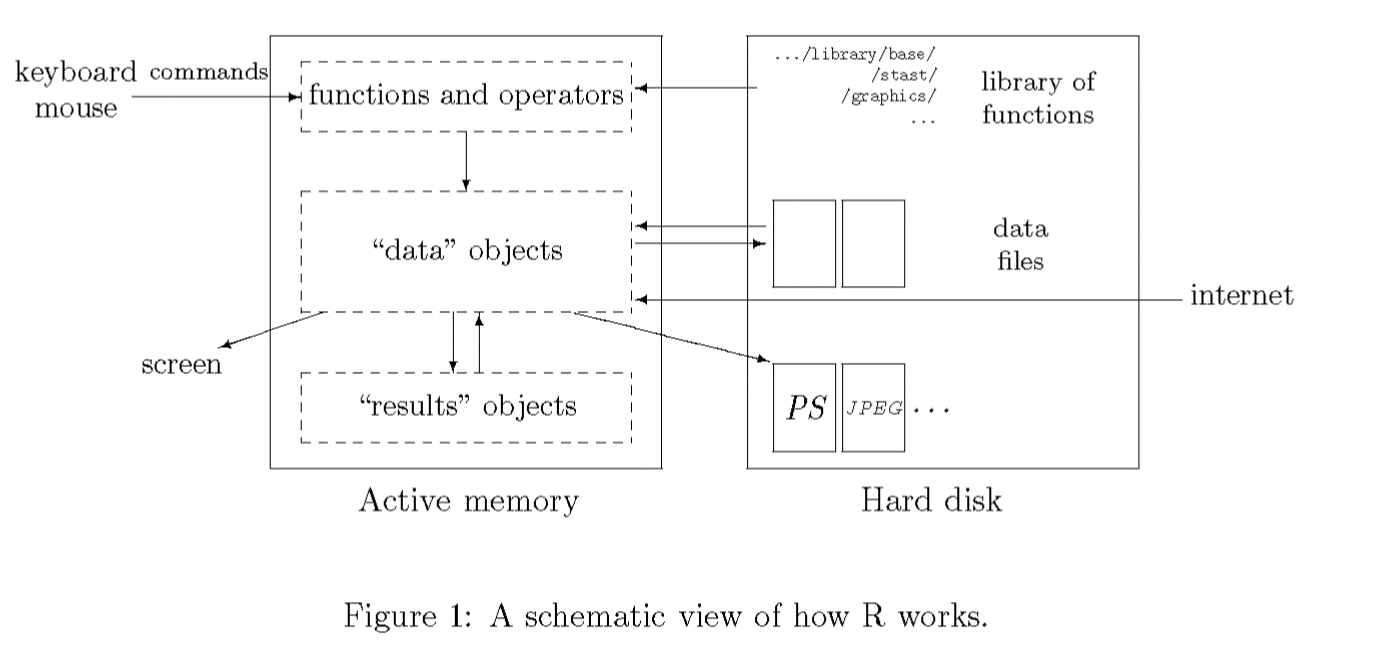
\includegraphics{./pics/como_piensa_R.png}

}

\caption{Cómo piensa R}

\end{figure}

En la sección anterior hemos visto como importar y gestionar variables
de un \textbf{dataframe}. En esta práctica vamos a ver cómo obtener los
descriptivos básicos. Es lo que se llama Análisis Exploratorio de los
Datos (Exploratory Data Analysis {[}EDA{]})

Lo primero que debemos hacer es cargar los datos de iam que habíamos
importado y modificado en la sesión anterior.

No indico ruta porque estoy en el directorio de trabajo y es donde está
el archivo.

\begin{Shaded}
\begin{Highlighting}[]
\NormalTok{iam }\OtherTok{\textless{}{-}} \FunctionTok{readRDS}\NormalTok{(}\StringTok{\textquotesingle{}iam.RDS\textquotesingle{}}\NormalTok{)}
\end{Highlighting}
\end{Shaded}

Si no fuese así, debería indicar la ruta entre las comillas. Por
ejemplo, si estuviese en un subdirectorio del de trabajo, debería
hacerlo así.

\begin{Shaded}
\begin{Highlighting}[]
\FunctionTok{readRDS}\NormalTok{(}\StringTok{\textquotesingle{}\_data/iam.RDS\textquotesingle{}}\NormalTok{)}
\end{Highlighting}
\end{Shaded}

Este código debería devolveros un error salvo que efectivamnte hayáis
colocado el archivo en ese subdirectorio\footnote{Recordad que siempre
  es mejor utilizar direccionamiento relativo (/\_data/iam.RDS) en vez
  de absoluto
  (`C:/Users/Usuario/Documents/SUB1/SUB2/SUB3/SUB4/SUB5/SUB6/dataiam.RDS')
  - atención a la dirección de la barra si copiasteis el path desde
  Windows}

\hypertarget{descriptivo-inicial-y-depuraciuxf3n.}{%
\section{Descriptivo inicial y
depuración.}\label{descriptivo-inicial-y-depuraciuxf3n.}}

Entre los objetivos del llamado Análisis Exploratorio de los Datos (EDA
o Exploratory Data Analysis) destacaría tres:

\begin{itemize}
\tightlist
\item
  Obtener una visión general de la distribución de tus variables tanto
  mediante los descriptivos como los gráficos adecuados para el tipo de
  variable.
\item
  Detectar valores anómalos por ser extremos (outliers), por no constar
  (missing) o por ser imposibles (error de medida o de introducción).
\item
  Visualizar relaciones bivariadas (también hay técnicas multivariadas,
  pero no las veremos en esta introducción) entre las variables del
  dataframe.
\item
  Una vez identificado todo lo anterior, podremos construir una primera
  foto de nuestra muestra.
\end{itemize}

Respecto a los valores anómalos, a veces podrán ser eliminados (errores
de introducción), pero en otras ocasiones tendremos que lidiar con ellos
en la construcción de los modelos y en la presentación de los
resultados.

Aunque no es una regla exacta, se suele decir que no te puedes fiar de
una variable que tenga más de un 10\% de valores perdidos (missing),
pero en ocasiones no te queda más remedio que utilizarlas. En estos
casos hay diversas técnicas de imputación de valores perdidos que
escapan a los objetivos de este curso.

Como habremos visto durante la clase, los descriptivos y gráficos
adecuados dependen de la escala de medida de la variable a describir.

R tiene algunos criterios para decidir que devolver cuando le pedimos
que haga un resumen (función \emph{summary}), pero para ello necesita
que la variable sea de la clase adecuada (numéric, integer, logical,
factor)

Utilizaremos el dataframe iam. Recordemos su estructura.

\begin{Shaded}
\begin{Highlighting}[]
\FunctionTok{str}\NormalTok{(iam)}
\end{Highlighting}
\end{Shaded}

\begin{verbatim}
'data.frame':   100 obs. of  9 variables:
 $ Id    : int  1 2 3 4 5 6 7 8 9 10 ...
 $ Age   : num  65.2 62.5 64.7 65.4 70.7 ...
 $ Sex   : int  1 0 0 0 0 0 1 0 0 0 ...
 $ Height: num  1.62 1.56 1.69 1.34 1.81 1.78 1.79 1.44 1.56 1.87 ...
 $ Weight: num  74.6 60.9 74.2 43.9 80.9 ...
 $ Smoke : int  0 0 0 0 1 0 0 1 0 0 ...
 $ ami   : int  0 0 0 0 0 0 0 1 0 0 ...
 $ age5  : Factor w/ 2 levels "[55,65]","(65,75]": 2 1 1 2 2 2 2 1 1 2 ...
 $ bmi   : num  28.4 25 26 24.5 24.7 ...
\end{verbatim}

Como se puede apreciar, algunas variables que deberían ser categóricas
están como tipo entero (int o integer), así que lo primero que vamos a
hacer es convertirlas en factores.

\begin{Shaded}
\begin{Highlighting}[]
\NormalTok{iam}\SpecialCharTok{$}\NormalTok{Sex}\OtherTok{\textless{}{-}}\FunctionTok{factor}\NormalTok{(iam}\SpecialCharTok{$}\NormalTok{Sex,}\AttributeTok{labels=}\FunctionTok{c}\NormalTok{(}\StringTok{\textquotesingle{}Men\textquotesingle{}}\NormalTok{,}\StringTok{\textquotesingle{}Women\textquotesingle{}}\NormalTok{))}
\end{Highlighting}
\end{Shaded}

Podríamos ir cambiando una a una, pero R cuenta con algunas funciones
que permiten cambiar simultáneamente varias variables que se van a
etiquetar de la misma manera. En nuestro caso son ami (Acute Myocardial
Infarction) y Smoke (Fuma sí/no) que van con 0 (No) y 1 (Yes).

\begin{verbatim}
Es recomendable utilizar una estrategia homogénea de etiquetado de valores de variable para facilitar conversiones posteriores.
\end{verbatim}

La familia de funciones \emph{apply} (\emph{apply, lapply, sapply,
tapply, mapply\ldots{}}) no son demasiado intuitivas, y se han
desarrollado funciones que permiten realizar los mismo ocn código más
intuitivo. Aunque incluya aquí un ejemplo, no es esencial conocerlas
para poder realizar este tipo de modificación.

\begin{Shaded}
\begin{Highlighting}[]
\NormalTok{iam[,}\FunctionTok{c}\NormalTok{(}\StringTok{\textquotesingle{}ami\textquotesingle{}}\NormalTok{,}\StringTok{\textquotesingle{}Smoke\textquotesingle{}}\NormalTok{)]}\OtherTok{\textless{}{-}}\FunctionTok{lapply}\NormalTok{(iam[,}\FunctionTok{c}\NormalTok{(}\StringTok{\textquotesingle{}ami\textquotesingle{}}\NormalTok{,}\StringTok{\textquotesingle{}Smoke\textquotesingle{}}\NormalTok{)],factor,}\AttributeTok{labels=}\FunctionTok{c}\NormalTok{(}\StringTok{\textquotesingle{}No\textquotesingle{}}\NormalTok{,}\StringTok{\textquotesingle{}Yes\textquotesingle{}}\NormalTok{))}
\FunctionTok{str}\NormalTok{(iam)}
\end{Highlighting}
\end{Shaded}

\begin{verbatim}
'data.frame':   100 obs. of  9 variables:
 $ Id    : int  1 2 3 4 5 6 7 8 9 10 ...
 $ Age   : num  65.2 62.5 64.7 65.4 70.7 ...
 $ Sex   : Factor w/ 2 levels "Men","Women": 2 1 1 1 1 1 2 1 1 1 ...
 $ Height: num  1.62 1.56 1.69 1.34 1.81 1.78 1.79 1.44 1.56 1.87 ...
 $ Weight: num  74.6 60.9 74.2 43.9 80.9 ...
 $ Smoke : Factor w/ 2 levels "No","Yes": 1 1 1 1 2 1 1 2 1 1 ...
 $ ami   : Factor w/ 2 levels "No","Yes": 1 1 1 1 1 1 1 2 1 1 ...
 $ age5  : Factor w/ 2 levels "[55,65]","(65,75]": 2 1 1 2 2 2 2 1 1 2 ...
 $ bmi   : num  28.4 25 26 24.5 24.7 ...
\end{verbatim}

Como podemos observar, en la nueva estructura (hemos modificado el
dataframe) las variables que antes eran de tipo entero, ahora son
factores.

Si ahora pedimos un primer resumen, observamos una serie de descriptivos
básicos.

\begin{Shaded}
\begin{Highlighting}[]
\FunctionTok{summary}\NormalTok{(iam)}
\end{Highlighting}
\end{Shaded}

\begin{verbatim}
       Id              Age           Sex         Height          Weight      
 Min.   :  1.00   Min.   :59.50   Men  :58   Min.   :1.150   Min.   : 30.31  
 1st Qu.: 25.75   1st Qu.:63.73   Women:42   1st Qu.:1.580   1st Qu.: 64.77  
 Median : 50.50   Median :65.24              Median :1.705   Median : 77.36  
 Mean   : 50.50   Mean   :65.14              Mean   :1.683   Mean   : 74.62  
 3rd Qu.: 75.25   3rd Qu.:66.70              3rd Qu.:1.790   3rd Qu.: 82.59  
 Max.   :100.00   Max.   :70.71              Max.   :1.960   Max.   :121.87  
 Smoke     ami          age5         bmi       
 No :60   No :50   [55,65]:47   Min.   :17.09  
 Yes:40   Yes:50   (65,75]:53   1st Qu.:24.25  
                                Median :25.42  
                                Mean   :26.05  
                                3rd Qu.:27.81  
                                Max.   :33.01  
\end{verbatim}

El paquete \emph{psych} ofrece más posibilidades. Recuerde que si no lo
tienen instalado debe instalarlo antes de llamar al paquete.

\begin{Shaded}
\begin{Highlighting}[]
\NormalTok{psych}\SpecialCharTok{::}\FunctionTok{describe}\NormalTok{(iam)}
\end{Highlighting}
\end{Shaded}

\begin{verbatim}
       vars   n  mean    sd median trimmed   mad   min    max range  skew
Id        1 100 50.50 29.01  50.50   50.50 37.06  1.00 100.00 99.00  0.00
Age       2 100 65.14  2.09  65.24   65.15  2.23 59.50  70.71 11.21 -0.04
Sex*      3 100  1.42  0.50   1.00    1.40  0.00  1.00   2.00  1.00  0.32
Height    4 100  1.68  0.16   1.71    1.69  0.16  1.15   1.96  0.81 -0.72
Weight    5 100 74.62 16.79  77.36   74.86 12.53 30.31 121.87 91.56 -0.11
Smoke*    6 100  1.40  0.49   1.00    1.38  0.00  1.00   2.00  1.00  0.40
ami*      7 100  1.50  0.50   1.50    1.50  0.74  1.00   2.00  1.00  0.00
age5*     8 100  1.53  0.50   2.00    1.54  0.00  1.00   2.00  1.00 -0.12
bmi       9 100 26.05  3.14  25.42   25.86  2.02 17.09  33.01 15.93  0.35
       kurtosis   se
Id        -1.24 2.90
Age       -0.32 0.21
Sex*      -1.92 0.05
Height     0.43 0.02
Weight     0.47 1.68
Smoke*    -1.86 0.05
ami*      -2.02 0.05
age5*     -2.01 0.05
bmi        0.41 0.31
\end{verbatim}

Desgraciadamente, aunque identifica las variables categóricas, utiliza
el valor numérico subyacente. Fíjese en la media de la variable Sex
(1.42).

A no olvidar:

\begin{itemize}
\tightlist
\item
  Echar un vistazo al mínimo y máximo. Esto nos permite detectar valores
  imposibles (por ejemplo una edad de 130 años, o un peso de 999).
\item
  Identificar si hay valores perdidos.
\item
  Estadísticos que nos dan una primera visión sobre la distribución.

  \begin{itemize}
  \tightlist
  \item
    Cercanía de la media a la mediana, desviación típica (recuerde que
    el coeficiente de variación es \(\frac{sd}{\overline{x}})\)
    expresado en \%).
  \item
    Media recortada (trimmed, por defecto recorta el 10\%) nos permite
    evaluar la influencia de los valores extremos.
  \item
    Asimetría (Skewness) y curtosis (Kurtosis) que nos permiten evaluar
    su parecido con una distribución normal, aunque solo con la
    estimación no es suficiente para llegar a una conclusión.
  \item
    MAD o Median Absolute Deviation, una medida robusta de la
    variabilidad que no es más que la mediana de los valores absolutos
    de distancias de cada valor a la mediana del conjunto.
    \(MAD=median([X_i-median{X}])\). b
  \item
    También aparece el error estándar (standard error o \(se(X)\)) que
    como veremos es importante en inferencia y que no se debe confundir
    con la desviación típica (standar deviation o \((sd)\)).
  \item
    No aparecen por defecto pero se pueden solicitar los cuartiles, en
    realidad los percentiles que deseemos. Recuerde que estas son
    medidas de posición, que también ayudan a describir nuestros datos.
  \end{itemize}
\end{itemize}

\begin{Shaded}
\begin{Highlighting}[]
\NormalTok{psych}\SpecialCharTok{::}\FunctionTok{describe}\NormalTok{(iam,}\AttributeTok{quant=}\FunctionTok{c}\NormalTok{(.}\DecValTok{1}\NormalTok{,.}\DecValTok{25}\NormalTok{,.}\DecValTok{5}\NormalTok{,.}\DecValTok{75}\NormalTok{,.}\DecValTok{9}\NormalTok{))}
\end{Highlighting}
\end{Shaded}

\begin{verbatim}
       vars   n  mean    sd median trimmed   mad   min    max range  skew
Id        1 100 50.50 29.01  50.50   50.50 37.06  1.00 100.00 99.00  0.00
Age       2 100 65.14  2.09  65.24   65.15  2.23 59.50  70.71 11.21 -0.04
Sex*      3 100  1.42  0.50   1.00    1.40  0.00  1.00   2.00  1.00  0.32
Height    4 100  1.68  0.16   1.71    1.69  0.16  1.15   1.96  0.81 -0.72
Weight    5 100 74.62 16.79  77.36   74.86 12.53 30.31 121.87 91.56 -0.11
Smoke*    6 100  1.40  0.49   1.00    1.38  0.00  1.00   2.00  1.00  0.40
ami*      7 100  1.50  0.50   1.50    1.50  0.74  1.00   2.00  1.00  0.00
age5*     8 100  1.53  0.50   2.00    1.54  0.00  1.00   2.00  1.00 -0.12
bmi       9 100 26.05  3.14  25.42   25.86  2.02 17.09  33.01 15.93  0.35
       kurtosis   se  Q0.1 Q0.25  Q0.5 Q0.75  Q0.9
Id        -1.24 2.90 10.90 25.75 50.50 75.25 90.10
Age       -0.32 0.21 62.53 63.73 65.24 66.70 68.12
Sex*      -1.92 0.05  1.00  1.00  1.00  2.00  2.00
Height     0.43 0.02  1.47  1.58  1.71  1.79  1.86
Weight     0.47 1.68 53.96 64.77 77.36 82.59 93.47
Smoke*    -1.86 0.05  1.00  1.00  1.00  2.00  2.00
ami*      -2.02 0.05  1.00  1.00  1.50  2.00  2.00
age5*     -2.01 0.05  1.00  1.00  2.00  2.00  2.00
bmi        0.41 0.31 23.20 24.25 25.42 27.81 31.30
\end{verbatim}

Con frecuencia necesitamos obtener los descriptivos en función de los
grupos que establezca una variable categórica. Para ello podemos
recurrir a la función \emph{by}, en la que indicamos cotjunto de datos a
describir (argumento en posición 1), índice o variable que establece los
grupos (argumento en posición 2) y función que queremos aplicar a cada
grupo establecido por la funcion índice sobre las variables incluidas en
el objeto que contiene los datos \emph{iam}.

No todas las funciones son aceptadas por by, pero \emph{psych::describe}
si lo es.

\begin{Shaded}
\begin{Highlighting}[]
\FunctionTok{by}\NormalTok{(iam,iam}\SpecialCharTok{$}\NormalTok{Sex,psych}\SpecialCharTok{::}\NormalTok{describe)}
\end{Highlighting}
\end{Shaded}

\begin{verbatim}
iam$Sex: Men
       vars  n  mean    sd median trimmed   mad   min    max range  skew
Id        1 58 49.64 30.61  48.50   49.50 40.03  2.00 100.00 98.00  0.05
Age       2 58 65.15  2.07  65.28   65.12  2.03 60.89  70.71  9.82  0.18
Sex*      3 58  1.00  0.00   1.00    1.00  0.00  1.00   1.00  0.00   NaN
Height    4 58  1.67  0.16   1.70    1.69  0.17  1.15   1.87  0.72 -1.07
Weight    5 58 70.31 12.45  75.19   71.70 10.51 30.31  84.79 54.48 -1.01
Smoke*    6 58  1.31  0.47   1.00    1.27  0.00  1.00   2.00  1.00  0.80
ami*      7 58  1.34  0.48   1.00    1.31  0.00  1.00   2.00  1.00  0.64
age5*     8 58  1.52  0.50   2.00    1.52  0.00  1.00   2.00  1.00 -0.07
bmi       9 58 24.96  1.10  24.68   24.94  1.16 22.92  27.88  4.97  0.32
       kurtosis   se
Id        -1.36 4.02
Age       -0.33 0.27
Sex*        NaN 0.00
Height     1.07 0.02
Weight     0.55 1.63
Smoke*    -1.38 0.06
ami*      -1.62 0.06
age5*     -2.03 0.07
bmi       -0.56 0.14
------------------------------------------------------------ 
iam$Sex: Women
       vars  n  mean    sd median trimmed   mad   min    max range  skew
Id        1 42 51.69 26.97  53.50   51.74 31.88  1.00  99.00 98.00 -0.06
Age       2 42 65.13  2.14  65.19   65.19  2.36 59.50  68.63  9.13 -0.32
Sex*      3 42  2.00  0.00   2.00    2.00  0.00  2.00   2.00  0.00   NaN
Height    4 42  1.70  0.16   1.72    1.70  0.16  1.39   1.96  0.57 -0.27
Weight    5 42 80.58 20.06  80.74   81.40 16.12 36.92 121.87 84.95 -0.37
Smoke*    6 42  1.52  0.51   2.00    1.53  0.00  1.00   2.00  1.00 -0.09
ami*      7 42  1.71  0.46   2.00    1.76  0.00  1.00   2.00  1.00 -0.92
age5*     8 42  1.55  0.50   2.00    1.56  0.00  1.00   2.00  1.00 -0.18
bmi       9 42 27.55  4.26  28.54   27.91  4.68 17.09  33.01 15.93 -0.66
       kurtosis   se
Id        -1.14 4.16
Age       -0.44 0.33
Sex*        NaN 0.00
Height    -0.79 0.02
Weight    -0.20 3.10
Smoke*    -2.04 0.08
ami*      -1.19 0.07
age5*     -2.01 0.08
bmi       -0.45 0.66
\end{verbatim}

Como se puede observar, la salida no está para ser publicada.

Como también habremos comentado en las clases de teoría, las variables
categóricas ofrecen menos posibilidades descriptivas (contienen menos
información) y su descripción univariada se va a reducir a dar las
frecuencias absolutas y relativas.

La obtención de una tabla de contingencia es relativamente fácil.

\begin{Shaded}
\begin{Highlighting}[]
\FunctionTok{table}\NormalTok{(iam}\SpecialCharTok{$}\NormalTok{Sex,iam}\SpecialCharTok{$}\NormalTok{Smoke)}
\end{Highlighting}
\end{Shaded}

\begin{verbatim}
       
        No Yes
  Men   40  18
  Women 20  22
\end{verbatim}

Y la de las frecuencias relativas por (condicionadas a) fila o columna,
también.

\begin{Shaded}
\begin{Highlighting}[]
\NormalTok{t1}\OtherTok{\textless{}{-}}\FunctionTok{table}\NormalTok{(iam}\SpecialCharTok{$}\NormalTok{Sex,iam}\SpecialCharTok{$}\NormalTok{Smoke)}
\FunctionTok{prop.table}\NormalTok{(t1,}\DecValTok{1}\NormalTok{) }\CommentTok{\# 1 le indca que son los \% sobre el total de fila, por eso suman 100\%.}
\end{Highlighting}
\end{Shaded}

\begin{verbatim}
       
               No       Yes
  Men   0.6896552 0.3103448
  Women 0.4761905 0.5238095
\end{verbatim}

Los de la tabla anterior son las proporciones de fumadores en el grupo
de mujeres (31\%) y de hombres (52\%).

Los de la siguiente son la proporción de hombres dentro de cada nivel de
la variable fumador (sí/no).

Entre los no fumadores el 66.7\% fueron hombres y el 33.3\% fueron
mujeres.

\begin{Shaded}
\begin{Highlighting}[]
\FunctionTok{prop.table}\NormalTok{(t1,}\DecValTok{2}\NormalTok{) }\CommentTok{\# 2 le indca que son los \% sobre el total de fila, por eso suman 100\%.}
\end{Highlighting}
\end{Shaded}

\begin{verbatim}
       
               No       Yes
  Men   0.6666667 0.4500000
  Women 0.3333333 0.5500000
\end{verbatim}

Existen funciones para ver los márgenes.

\begin{Shaded}
\begin{Highlighting}[]
\FunctionTok{addmargins}\NormalTok{ (}\FunctionTok{table}\NormalTok{(iam}\SpecialCharTok{$}\NormalTok{Sex,iam}\SpecialCharTok{$}\NormalTok{Smoke))}
\end{Highlighting}
\end{Shaded}

\begin{verbatim}
       
         No Yes Sum
  Men    40  18  58
  Women  20  22  42
  Sum    60  40 100
\end{verbatim}

Ir variable a variable no es lo que necesitamos cuando queremos resumir
muchas variables, por lo que algunos paquetes facilitan obtener esta
información de varias variables a la vez.

\begin{Shaded}
\begin{Highlighting}[]
\NormalTok{tableone}\SpecialCharTok{::}\FunctionTok{CreateCatTable}\NormalTok{(}\AttributeTok{data=}\NormalTok{iam,}\AttributeTok{vars=}\FunctionTok{c}\NormalTok{(}\StringTok{\textquotesingle{}Smoke\textquotesingle{}}\NormalTok{,}\StringTok{\textquotesingle{}ami\textquotesingle{}}\NormalTok{,}\StringTok{\textquotesingle{}age5\textquotesingle{}}\NormalTok{),}\AttributeTok{strata =} \StringTok{\textquotesingle{}Sex\textquotesingle{}}\NormalTok{,}\AttributeTok{test =}\NormalTok{ F)}
\end{Highlighting}
\end{Shaded}

\begin{verbatim}
                    Stratified by Sex
                     Men        Women     
  n                  58         42        
  Smoke = Yes (%)    18 (31.0)  22 (52.4) 
  ami = Yes (%)      20 (34.5)  30 (71.4) 
  age5 = (65,75] (%) 30 (51.7)  23 (54.8) 
\end{verbatim}

Incluso son capaces de distinguir el tipo de variable para utilizar el
descriptor adecuado.

\begin{Shaded}
\begin{Highlighting}[]
\NormalTok{tableone}\SpecialCharTok{::}\FunctionTok{CreateTableOne}\NormalTok{ (}\AttributeTok{data=}\NormalTok{iam[,}\SpecialCharTok{{-}}\DecValTok{1}\NormalTok{],}\AttributeTok{strata =} \StringTok{\textquotesingle{}Sex\textquotesingle{}}\NormalTok{,}\AttributeTok{test =}\NormalTok{ F)}
\end{Highlighting}
\end{Shaded}

\begin{verbatim}
                    Stratified by Sex
                     Men           Women         
  n                     58            42         
  Age (mean (SD))    65.15 (2.07)  65.13 (2.14)  
  Sex = Women (%)        0 ( 0.0)     42 (100.0) 
  Height (mean (SD))  1.67 (0.16)   1.70 (0.16)  
  Weight (mean (SD)) 70.31 (12.45) 80.58 (20.06) 
  Smoke = Yes (%)       18 (31.0)     22 ( 52.4) 
  ami = Yes (%)         20 (34.5)     30 ( 71.4) 
  age5 = (65,75] (%)    30 (51.7)     23 ( 54.8) 
  bmi (mean (SD))    24.96 (1.10)  27.55 (4.26)  
\end{verbatim}

Algunos incluso devuelven información gráfica.

\begin{Shaded}
\begin{Highlighting}[]
\FunctionTok{print}\NormalTok{(summarytools}\SpecialCharTok{::}\FunctionTok{dfSummary}\NormalTok{(iam[,}\SpecialCharTok{{-}}\DecValTok{1}\NormalTok{],}
                        \AttributeTok{plain.ascii  =} \ConstantTok{FALSE}\NormalTok{,}
          \AttributeTok{style        =} \StringTok{\textquotesingle{}grid\textquotesingle{}}\NormalTok{,}
          \AttributeTok{graph.magnif =} \FloatTok{0.85}\NormalTok{,}
          \AttributeTok{varnumbers =} \ConstantTok{FALSE}\NormalTok{,}
          \AttributeTok{valid.col    =} \ConstantTok{FALSE}\NormalTok{,}
          \CommentTok{\# tmp.img.dir  = "/tmp"}
\NormalTok{          ),}\AttributeTok{method =} \StringTok{\textquotesingle{}render\textquotesingle{}}\NormalTok{)}
\end{Highlighting}
\end{Shaded}

\begin{longtable}[]{@{}
  >{\raggedright\arraybackslash}p{(\columnwidth - 8\tabcolsep) * \real{0.2000}}
  >{\raggedright\arraybackslash}p{(\columnwidth - 8\tabcolsep) * \real{0.2000}}
  >{\raggedright\arraybackslash}p{(\columnwidth - 8\tabcolsep) * \real{0.2000}}
  >{\raggedright\arraybackslash}p{(\columnwidth - 8\tabcolsep) * \real{0.2000}}
  >{\centering\arraybackslash}p{(\columnwidth - 8\tabcolsep) * \real{0.2000}}@{}}
\toprule()
\begin{minipage}[b]{\linewidth}\centering
\textbf{Variable}
\end{minipage} & \begin{minipage}[b]{\linewidth}\centering
\textbf{Stats / Values}
\end{minipage} & \begin{minipage}[b]{\linewidth}\centering
\textbf{Freqs (\% of Valid)}
\end{minipage} & \begin{minipage}[b]{\linewidth}\centering
\textbf{Graph}
\end{minipage} & \begin{minipage}[b]{\linewidth}\centering
\textbf{Missing}
\end{minipage} \\
\midrule()
\endhead
Age {[}numeric{]} & \begin{minipage}[t]{\linewidth}\raggedright
\begin{longtable}[]{@{}l@{}}
\toprule()
\endhead
Mean (sd) : 65.1 (2.1) \\
min ≤ med ≤ max: \\
59.5 ≤ 65.2 ≤ 70.7 \\
IQR (CV) : 3 (0) \\
\bottomrule()
\end{longtable}
\end{minipage} & 100 distinct values & & 0 (0.0\%) \\
Sex {[}factor{]} & \begin{minipage}[t]{\linewidth}\raggedright
\begin{longtable}[]{@{}l@{}}
\toprule()
\endhead
1. Men \\
2. Women \\
\bottomrule()
\end{longtable}
\end{minipage} & \begin{minipage}[t]{\linewidth}\raggedright
\begin{longtable}[]{@{}rlrl@{}}
\toprule()
\endhead
58 & ( & 58.0\% & ) \\
42 & ( & 42.0\% & ) \\
\bottomrule()
\end{longtable}
\end{minipage} & & 0 (0.0\%) \\
Height {[}numeric{]} & \begin{minipage}[t]{\linewidth}\raggedright
\begin{longtable}[]{@{}l@{}}
\toprule()
\endhead
Mean (sd) : 1.7 (0.2) \\
min ≤ med ≤ max: \\
1.1 ≤ 1.7 ≤ 2 \\
IQR (CV) : 0.2 (0.1) \\
\bottomrule()
\end{longtable}
\end{minipage} & 38 distinct values & & 0 (0.0\%) \\
Weight {[}numeric{]} & \begin{minipage}[t]{\linewidth}\raggedright
\begin{longtable}[]{@{}l@{}}
\toprule()
\endhead
Mean (sd) : 74.6 (16.8) \\
min ≤ med ≤ max: \\
30.3 ≤ 77.4 ≤ 121.9 \\
IQR (CV) : 17.8 (0.2) \\
\bottomrule()
\end{longtable}
\end{minipage} & 76 distinct values & & 0 (0.0\%) \\
Smoke {[}factor{]} & \begin{minipage}[t]{\linewidth}\raggedright
\begin{longtable}[]{@{}l@{}}
\toprule()
\endhead
1. No \\
2. Yes \\
\bottomrule()
\end{longtable}
\end{minipage} & \begin{minipage}[t]{\linewidth}\raggedright
\begin{longtable}[]{@{}rlrl@{}}
\toprule()
\endhead
60 & ( & 60.0\% & ) \\
40 & ( & 40.0\% & ) \\
\bottomrule()
\end{longtable}
\end{minipage} & & 0 (0.0\%) \\
ami {[}factor{]} & \begin{minipage}[t]{\linewidth}\raggedright
\begin{longtable}[]{@{}l@{}}
\toprule()
\endhead
1. No \\
2. Yes \\
\bottomrule()
\end{longtable}
\end{minipage} & \begin{minipage}[t]{\linewidth}\raggedright
\begin{longtable}[]{@{}rlrl@{}}
\toprule()
\endhead
50 & ( & 50.0\% & ) \\
50 & ( & 50.0\% & ) \\
\bottomrule()
\end{longtable}
\end{minipage} & & 0 (0.0\%) \\
age5 {[}factor{]} & \begin{minipage}[t]{\linewidth}\raggedright
\begin{longtable}[]{@{}l@{}}
\toprule()
\endhead
1. {[}55,65{]} \\
2. (65,75{]} \\
\bottomrule()
\end{longtable}
\end{minipage} & \begin{minipage}[t]{\linewidth}\raggedright
\begin{longtable}[]{@{}rlrl@{}}
\toprule()
\endhead
47 & ( & 47.0\% & ) \\
53 & ( & 53.0\% & ) \\
\bottomrule()
\end{longtable}
\end{minipage} & & 0 (0.0\%) \\
bmi {[}numeric{]} & \begin{minipage}[t]{\linewidth}\raggedright
\begin{longtable}[]{@{}l@{}}
\toprule()
\endhead
Mean (sd) : 26 (3.1) \\
min ≤ med ≤ max: \\
17.1 ≤ 25.4 ≤ 33 \\
IQR (CV) : 3.6 (0.1) \\
\bottomrule()
\end{longtable}
\end{minipage} & 77 distinct values & & 0 (0.0\%) \\
\bottomrule()
\end{longtable}

En cualquier caso siguen siendo tablas que no están listas para ser
publicadas.

Si dio tiempo, en la última clase deberíamos haber visto una tabla
construida como \emph{``publication-ready tables''}.

Aquí incluyo un ejemplo, con los datos utilizados en esta sesión.

\begin{table}
\caption*{
{\large Table 1. Descriptive statistics of the sample by Sex}
} 
\fontsize{12.0pt}{14.4pt}\selectfont
\begin{tabular*}{\linewidth}{@{\extracolsep{\fill}}lcc}
\toprule
\textbf{Characteristic} & \textbf{Men}  N = 58\textsuperscript{\textit{1}} & \textbf{Women}  N = 42\textsuperscript{\textit{1}} \\ 
\midrule\addlinespace[2.5pt]
Age & 65.28 (63.74, 66.54) & 65.19 (63.72, 66.78) \\ 
Height & 1.70 (1.57, 1.79) & 1.72 (1.58, 1.79) \\ 
Weight & 75 (61, 81) & 81 (73, 93) \\ 
Smoke & 18 (31\%) & 22 (52\%) \\ 
AMI & 20 (34\%) & 30 (71\%) \\ 
Age group &  &  \\ 
    [55,65] & 28 (48\%) & 19 (45\%) \\ 
    (65,75] & 30 (52\%) & 23 (55\%) \\ 
BMI & 24.68 (24.20, 25.79) & 28.54 (24.48, 31.30) \\ 
\bottomrule
\end{tabular*}
\begin{minipage}{\linewidth}
\textsuperscript{\textit{1}}Median (Q1, Q3); n (\%)\\
\end{minipage}
\end{table}

\hypertarget{gruxe1ficos-simples.}{%
\subsection{Gráficos simples.}\label{gruxe1ficos-simples.}}

Incluyo aquí algunos gráficos elaborados con las opciones gráficas en lo
que he denominado \emph{base R}. No serán los que utilizaremos para
publicar, pero son perfectamente correctos.

\hypertarget{gruxe1ficos.-variables-categuxf3ricas.}{%
\subsubsection{Gráficos. Variables
categóricas.}\label{gruxe1ficos.-variables-categuxf3ricas.}}

\hypertarget{gruxe1ficos-de-columnas.}{%
\paragraph{Gráficos de columnas.}\label{gruxe1ficos-de-columnas.}}

Curiosamente es uno de los gráficos más sencillos y sin embargo en base
R su personalización es laboriosa, entre otras cosas porque necesita
construir previamente una tabla.

\begin{Shaded}
\begin{Highlighting}[]
\NormalTok{t2}\OtherTok{\textless{}{-}}\DecValTok{100}\SpecialCharTok{*}\FunctionTok{prop.table}\NormalTok{(}\FunctionTok{table}\NormalTok{(iam}\SpecialCharTok{$}\NormalTok{Smoke,iam}\SpecialCharTok{$}\NormalTok{Sex),}\DecValTok{2}\NormalTok{)}
\NormalTok{p}\OtherTok{\textless{}{-}}\FunctionTok{barplot}\NormalTok{(t2,}\AttributeTok{beside=}\NormalTok{T,}\AttributeTok{col=}\FunctionTok{c}\NormalTok{(}\StringTok{\textquotesingle{}cadetblue\textquotesingle{}}\NormalTok{,}\StringTok{\textquotesingle{}red\textquotesingle{}}\NormalTok{),}
        \AttributeTok{ylim=}\FunctionTok{c}\NormalTok{(}\DecValTok{0}\NormalTok{,}\DecValTok{100}\NormalTok{),}
        \AttributeTok{ylab=}\StringTok{\textquotesingle{}\%\textquotesingle{}}\NormalTok{,}
        \AttributeTok{xlab=}\StringTok{\textquotesingle{}Sex\textquotesingle{}}\NormalTok{)}
\FunctionTok{text}\NormalTok{(}\AttributeTok{x =} \FunctionTok{c}\NormalTok{(}\StringTok{\textquotesingle{}uno\textquotesingle{}}\NormalTok{,}\StringTok{\textquotesingle{}dos\textquotesingle{}}\NormalTok{))}
\end{Highlighting}
\end{Shaded}

\begin{verbatim}
Warning in xy.coords(x, y, recycle = TRUE, setLab = FALSE): NAs introducidos
por coerción
\end{verbatim}

\begin{figure}[H]

{\centering 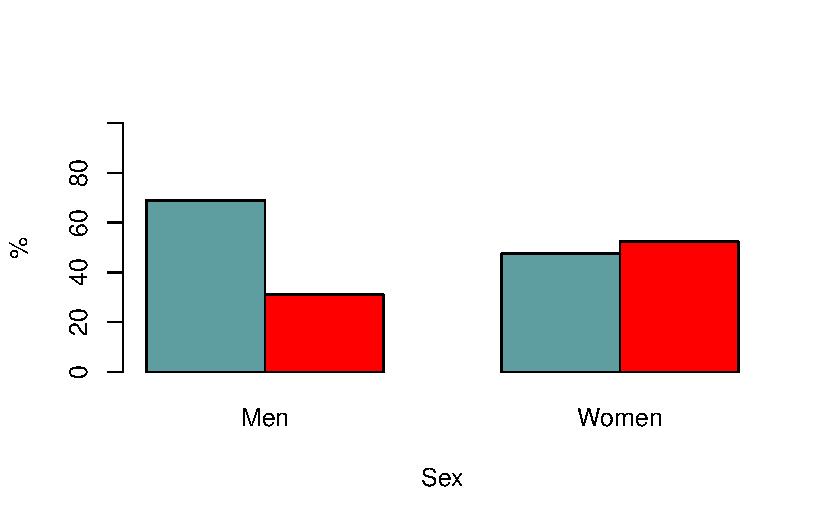
\includegraphics{./PR_4_lect_files/figure-pdf/unnamed-chunk-18-1.pdf}

}

\end{figure}

\hypertarget{gruxe1ficos.-variables-continuas.}{%
\subsubsection{Gráficos. Variables
continuas.}\label{gruxe1ficos.-variables-continuas.}}

Algo similar va a ocurrir con respecto a las posibilidades gráficas en
la descripción univariada.

Desarrollamos aquí los gráficos vistos durante las clases.

\hypertarget{histograma}{%
\paragraph{Histograma}\label{histograma}}

\begin{Shaded}
\begin{Highlighting}[]
\FunctionTok{hist}\NormalTok{(iam}\SpecialCharTok{$}\NormalTok{Age) }\CommentTok{\# las opciones ayudan a mejorar la presentación. }
\end{Highlighting}
\end{Shaded}

\begin{figure}[H]

{\centering 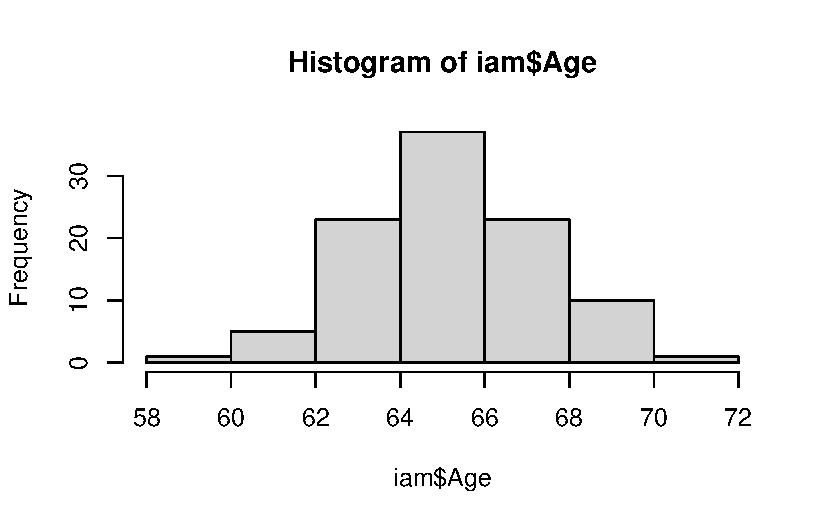
\includegraphics{./PR_4_lect_files/figure-pdf/unnamed-chunk-19-1.pdf}

}

\end{figure}

\begin{Shaded}
\begin{Highlighting}[]
\FunctionTok{hist}\NormalTok{(iam}\SpecialCharTok{$}\NormalTok{Age,}\AttributeTok{freq=}\NormalTok{F,}\AttributeTok{col=}\StringTok{"blue"}\NormalTok{,}\AttributeTok{xlab=}\StringTok{"Edad"}\NormalTok{) }\CommentTok{\#prob=T es lo mismo que freq=F}
\FunctionTok{lines}\NormalTok{(}\FunctionTok{density}\NormalTok{(iam}\SpecialCharTok{$}\NormalTok{Age)) }\CommentTok{\# para que dibuje la función de densidad. Necesita prob=T (*)}
\end{Highlighting}
\end{Shaded}

\begin{figure}[H]

{\centering 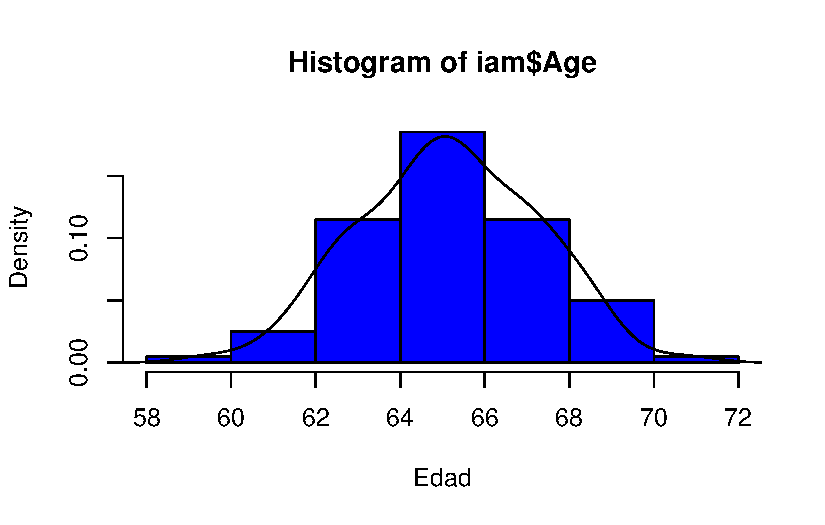
\includegraphics{./PR_4_lect_files/figure-pdf/unnamed-chunk-19-2.pdf}

}

\end{figure}

Se puede sofisticar algo más.

Esta representación fusiona los dos histogramas y juega con la
transparencia para comparar su distribuciones.

\begin{Shaded}
\begin{Highlighting}[]
\FunctionTok{hist}\NormalTok{(iam}\SpecialCharTok{$}\NormalTok{Age[iam}\SpecialCharTok{$}\NormalTok{Sex}\SpecialCharTok{==}\StringTok{"Men"}\NormalTok{],}\AttributeTok{freq=}\NormalTok{F,}\AttributeTok{col=}\FunctionTok{rgb}\NormalTok{(}\DecValTok{1}\NormalTok{,}\DecValTok{0}\NormalTok{,}\DecValTok{0}\NormalTok{,}\DecValTok{1}\SpecialCharTok{/}\DecValTok{5}\NormalTok{),}\AttributeTok{xlab=}\StringTok{\textquotesingle{}Age\textquotesingle{}}\NormalTok{,}\AttributeTok{main=}\StringTok{\textquotesingle{}Histogram of Age by Sex\textquotesingle{}}\NormalTok{)}
\FunctionTok{hist}\NormalTok{(iam}\SpecialCharTok{$}\NormalTok{Age[iam}\SpecialCharTok{$}\NormalTok{Sex}\SpecialCharTok{==}\StringTok{"Women"}\NormalTok{],}\AttributeTok{freq=}\NormalTok{F,}\AttributeTok{col=}\FunctionTok{rgb}\NormalTok{(}\DecValTok{0}\NormalTok{,}\DecValTok{0}\NormalTok{,}\DecValTok{1}\NormalTok{,}\DecValTok{1}\SpecialCharTok{/}\DecValTok{5}\NormalTok{),}\AttributeTok{add=}\NormalTok{T,}\AttributeTok{xlab=}\StringTok{\textquotesingle{}Age\textquotesingle{}}\NormalTok{)}
\end{Highlighting}
\end{Shaded}

\begin{figure}[H]

{\centering 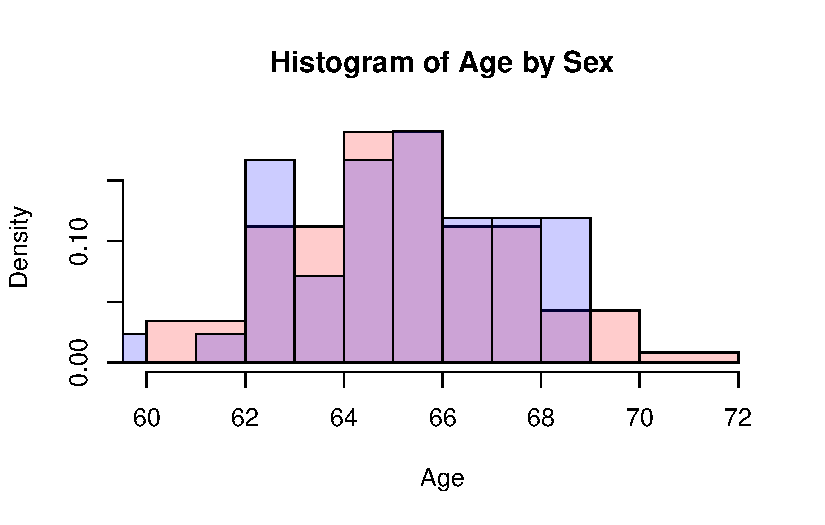
\includegraphics{./PR_4_lect_files/figure-pdf/unnamed-chunk-20-1.pdf}

}

\end{figure}

\begin{Shaded}
\begin{Highlighting}[]
\CommentTok{\#Es necesario usar freq=T porque si saca las absolutas el grupo más grande destacará sobre el grupo más pequeño.}
\end{Highlighting}
\end{Shaded}

\hypertarget{boxplot}{%
\paragraph{Boxplot}\label{boxplot}}

\hypertarget{una-variable.}{%
\subparagraph{Una variable.}\label{una-variable.}}

\begin{Shaded}
\begin{Highlighting}[]
\FunctionTok{boxplot}\NormalTok{(iam}\SpecialCharTok{$}\NormalTok{Age)}
\end{Highlighting}
\end{Shaded}

\begin{figure}[H]

{\centering 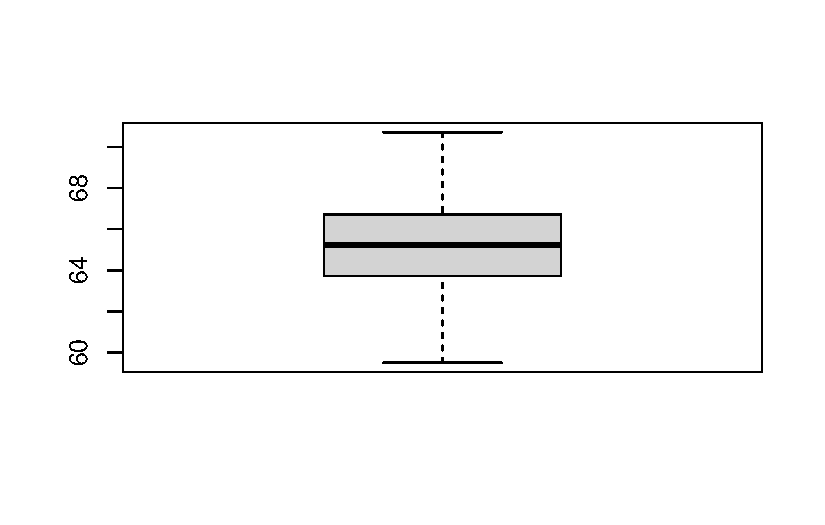
\includegraphics{./PR_4_lect_files/figure-pdf/unnamed-chunk-21-1.pdf}

}

\end{figure}

\begin{Shaded}
\begin{Highlighting}[]
\FunctionTok{boxplot}\NormalTok{(iam}\SpecialCharTok{$}\NormalTok{Age,}\AttributeTok{col=}\StringTok{"red"}\NormalTok{)}
\FunctionTok{text}\NormalTok{(}\FloatTok{1.25}\NormalTok{,}\FunctionTok{median}\NormalTok{(iam}\SpecialCharTok{$}\NormalTok{Age),}\FunctionTok{round}\NormalTok{(}\FunctionTok{median}\NormalTok{(iam}\SpecialCharTok{$}\NormalTok{Age),}\DecValTok{2}\NormalTok{)) }\CommentTok{\# función gráfica de bajo nivel.}
\end{Highlighting}
\end{Shaded}

\begin{figure}[H]

{\centering 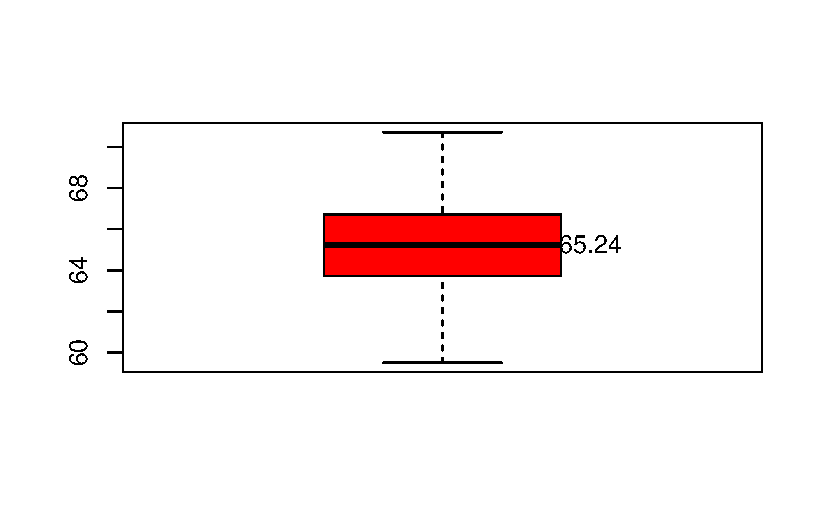
\includegraphics{./PR_4_lect_files/figure-pdf/unnamed-chunk-21-2.pdf}

}

\end{figure}

\hypertarget{por-grupos-de-otra-variable-categuxf3rica.}{%
\subparagraph{Por grupos de otra variable
categórica.}\label{por-grupos-de-otra-variable-categuxf3rica.}}

Incluimos algunas ociones de configuración.

Las etiquetas salen porque las hemos deficido en el factor, de otra
forma saldrían los valores (0,1)

\begin{Shaded}
\begin{Highlighting}[]
\FunctionTok{boxplot}\NormalTok{(}\AttributeTok{formula=}\NormalTok{Age}\SpecialCharTok{\textasciitilde{}}\NormalTok{Sex,}\AttributeTok{data=}\NormalTok{iam,}
        \AttributeTok{col=}\FunctionTok{c}\NormalTok{(}\StringTok{\textquotesingle{}orange\textquotesingle{}}\NormalTok{,}\StringTok{\textquotesingle{}purple\textquotesingle{}}\NormalTok{)}
\NormalTok{        )}
\end{Highlighting}
\end{Shaded}

\begin{figure}[H]

{\centering 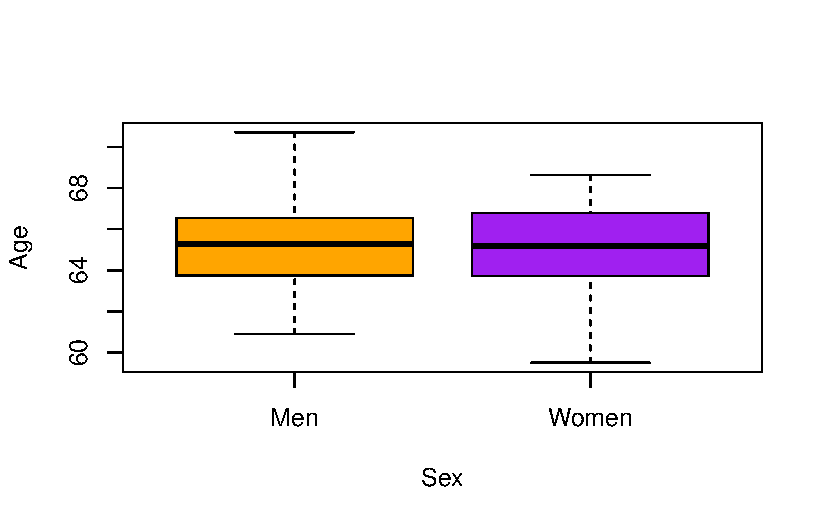
\includegraphics{./PR_4_lect_files/figure-pdf/unnamed-chunk-22-1.pdf}

}

\end{figure}

\hypertarget{stemleaf}{%
\paragraph{Stem\&Leaf}\label{stemleaf}}

Lo incluyo por cuestiones históricas y porque realmente aporta
información que el histograma no, pero es raro ya ver este gráfico.

\begin{Shaded}
\begin{Highlighting}[]
\FunctionTok{stem}\NormalTok{(iam}\SpecialCharTok{$}\NormalTok{Age)}
\end{Highlighting}
\end{Shaded}

\begin{verbatim}

  The decimal point is at the |

  58 | 5
  60 | 92579
  62 | 1235567788890114557799
  64 | 0112334455577788890112233344445555799
  66 | 002334456788802222233455
  68 | 1122344662
  70 | 7
\end{verbatim}

\hypertarget{gruxe1fico-q-q.}{%
\paragraph{Gráfico Q-Q.}\label{gruxe1fico-q-q.}}

Gráfica cuantil-cuantil frente a distribución normal.

Este gráfico es muy útil y sirve para analizar visualmente si una
distribución empírica (nuestros datos observados) sigue razonablemente
bien una distribución normal\footnote{En realidad se puede comparar con
  otras distribuciones teóricas, pero la que nos interesa aquí es la
  distribución normal}. Cuando la sigue, los puntos se distribuyen cerca
de la línea.

Para ello enfrentan los datos observados frente a los cuantiles que
ocuparían en una distribución, en este caso normal.

Las coordenadas en cada eje para cada punto se construyen de la
siguiente manera\footnote{Si no recuerdo mal, SPSS representa este
  gráfico invirtiendo los ejes, pero la interpretación es muy similar.}.

En el eje de ordenadas (eje y) representa la posición que ocupan los
valores observados expresada en cuantiles desde el centro de la
distribución empírica. En el eje de abscisas (eje x) se representa la
posición que ocuparían dichos valores en una distribución teórica normal
perfecta con la misma media y desviación típica que la distribución
empírica.

Si la distancia (expresada en cuantiles) a la que está un punto
observado en la distribución empírica coincidiese perfectamente con la
distancia (expresada en cuantiles) a la que estaría ese mismo punto en
una distribución normal perfecta con la misma media y desviación típica
que la de la distribución empírica, todos los puntos se colocarían en la
diagonal diagonal. Si se apartan, es que los puntos no están donde se
les espera, informando de asimetrías en las colas, distribuciones
bimodales, existencia de valores atípicos\ldots{}

Hace falta cierta experiencia para interpretar los detalles finos, pero
es un gráfico bastante intuitivo para identificar problemas con la
normalidad de la variable incluso al ojo menos experimentado.

\begin{Shaded}
\begin{Highlighting}[]
\NormalTok{qqnorm }\CommentTok{\#(Gráfico cuantil{-}cuantil de distribución de variable problema frente a distribución normal con misma media y desviación típica que la de la variable problema).}
\end{Highlighting}
\end{Shaded}

\begin{verbatim}
function (y, ...) 
UseMethod("qqnorm")
<bytecode: 0x000002caec894148>
<environment: namespace:stats>
\end{verbatim}

\begin{Shaded}
\begin{Highlighting}[]
\FunctionTok{qqnorm}\NormalTok{(iam}\SpecialCharTok{$}\NormalTok{Age)}
\FunctionTok{qqline}\NormalTok{(iam}\SpecialCharTok{$}\NormalTok{Age)}
\end{Highlighting}
\end{Shaded}

\begin{figure}[H]

{\centering 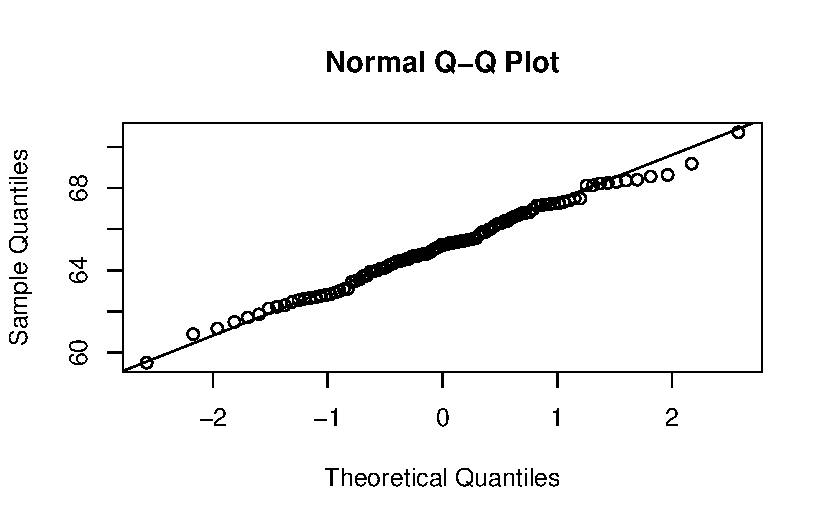
\includegraphics{./PR_4_lect_files/figure-pdf/unnamed-chunk-24-1.pdf}

}

\end{figure}

\hypertarget{gruxe1fico-de-dispersiuxf3n-o-scatter-plot.}{%
\subsection{Gráfico de dispersión o scatter
plot.}\label{gruxe1fico-de-dispersiuxf3n-o-scatter-plot.}}

En este representamos la relación bivariada entre dos variables
cuantitativas, preferentemente continuas.

\begin{Shaded}
\begin{Highlighting}[]
\FunctionTok{plot}\NormalTok{(iam}\SpecialCharTok{$}\NormalTok{Age,iam}\SpecialCharTok{$}\NormalTok{bmi,}\AttributeTok{main=}\StringTok{\textquotesingle{}Scatter plot BMI by Age\textquotesingle{}}\NormalTok{,}
     \AttributeTok{xlab=}\StringTok{\textquotesingle{}Age [yrs.]\textquotesingle{}}\NormalTok{,}
     \AttributeTok{ylab=}\FunctionTok{expression}\NormalTok{(}\FunctionTok{paste}\NormalTok{(}\StringTok{\textquotesingle{}Body Mass Index [\textquotesingle{}}\NormalTok{,Kg}\SpecialCharTok{/}\NormalTok{m}\SpecialCharTok{\^{}}\DecValTok{2}\NormalTok{,}\StringTok{\textquotesingle{}]\textquotesingle{}}\NormalTok{)) }\CommentTok{\#Es posible insertar fórmulas, aunque no siempre es fácil.}
\NormalTok{)}
\end{Highlighting}
\end{Shaded}

\begin{figure}[H]

{\centering 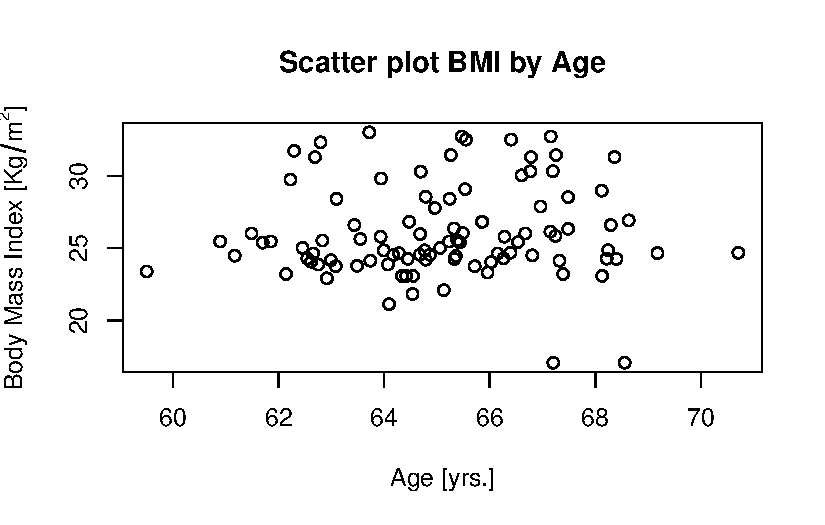
\includegraphics{./PR_4_lect_files/figure-pdf/unnamed-chunk-25-1.pdf}

}

\end{figure}

Si tuviésemos que ir una a una, supondría mucho trabajo. Existen
funciones que nos pueden devolver múltiples tipos de relación
simultáneamente.

\begin{Shaded}
\begin{Highlighting}[]
\FunctionTok{pairs}\NormalTok{(iam[,}\FunctionTok{c}\NormalTok{(}\StringTok{\textquotesingle{}Age\textquotesingle{}}\NormalTok{,}\StringTok{\textquotesingle{}Height\textquotesingle{}}\NormalTok{,}\StringTok{\textquotesingle{}Weight\textquotesingle{}}\NormalTok{,}\StringTok{\textquotesingle{}bmi\textquotesingle{}}\NormalTok{)])}
\end{Highlighting}
\end{Shaded}

\begin{figure}[H]

{\centering 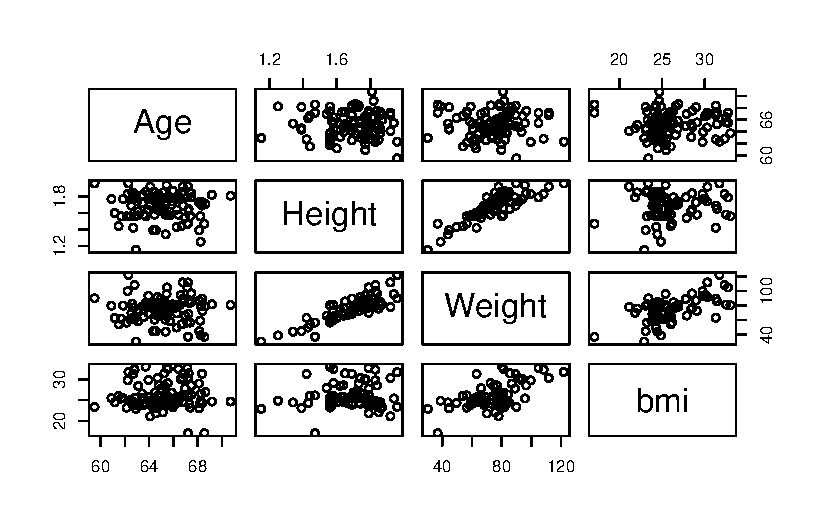
\includegraphics{./PR_4_lect_files/figure-pdf/unnamed-chunk-26-1.pdf}

}

\end{figure}

Como pasaba con las tablas, estos gráficos no son aún
\emph{`Publication-ready Graphs'}. Dado que este tipo de gráficos no son
necesarios para superar el bloque, si da tiempo hablaremos de cómo
crearlos en la última sesión.

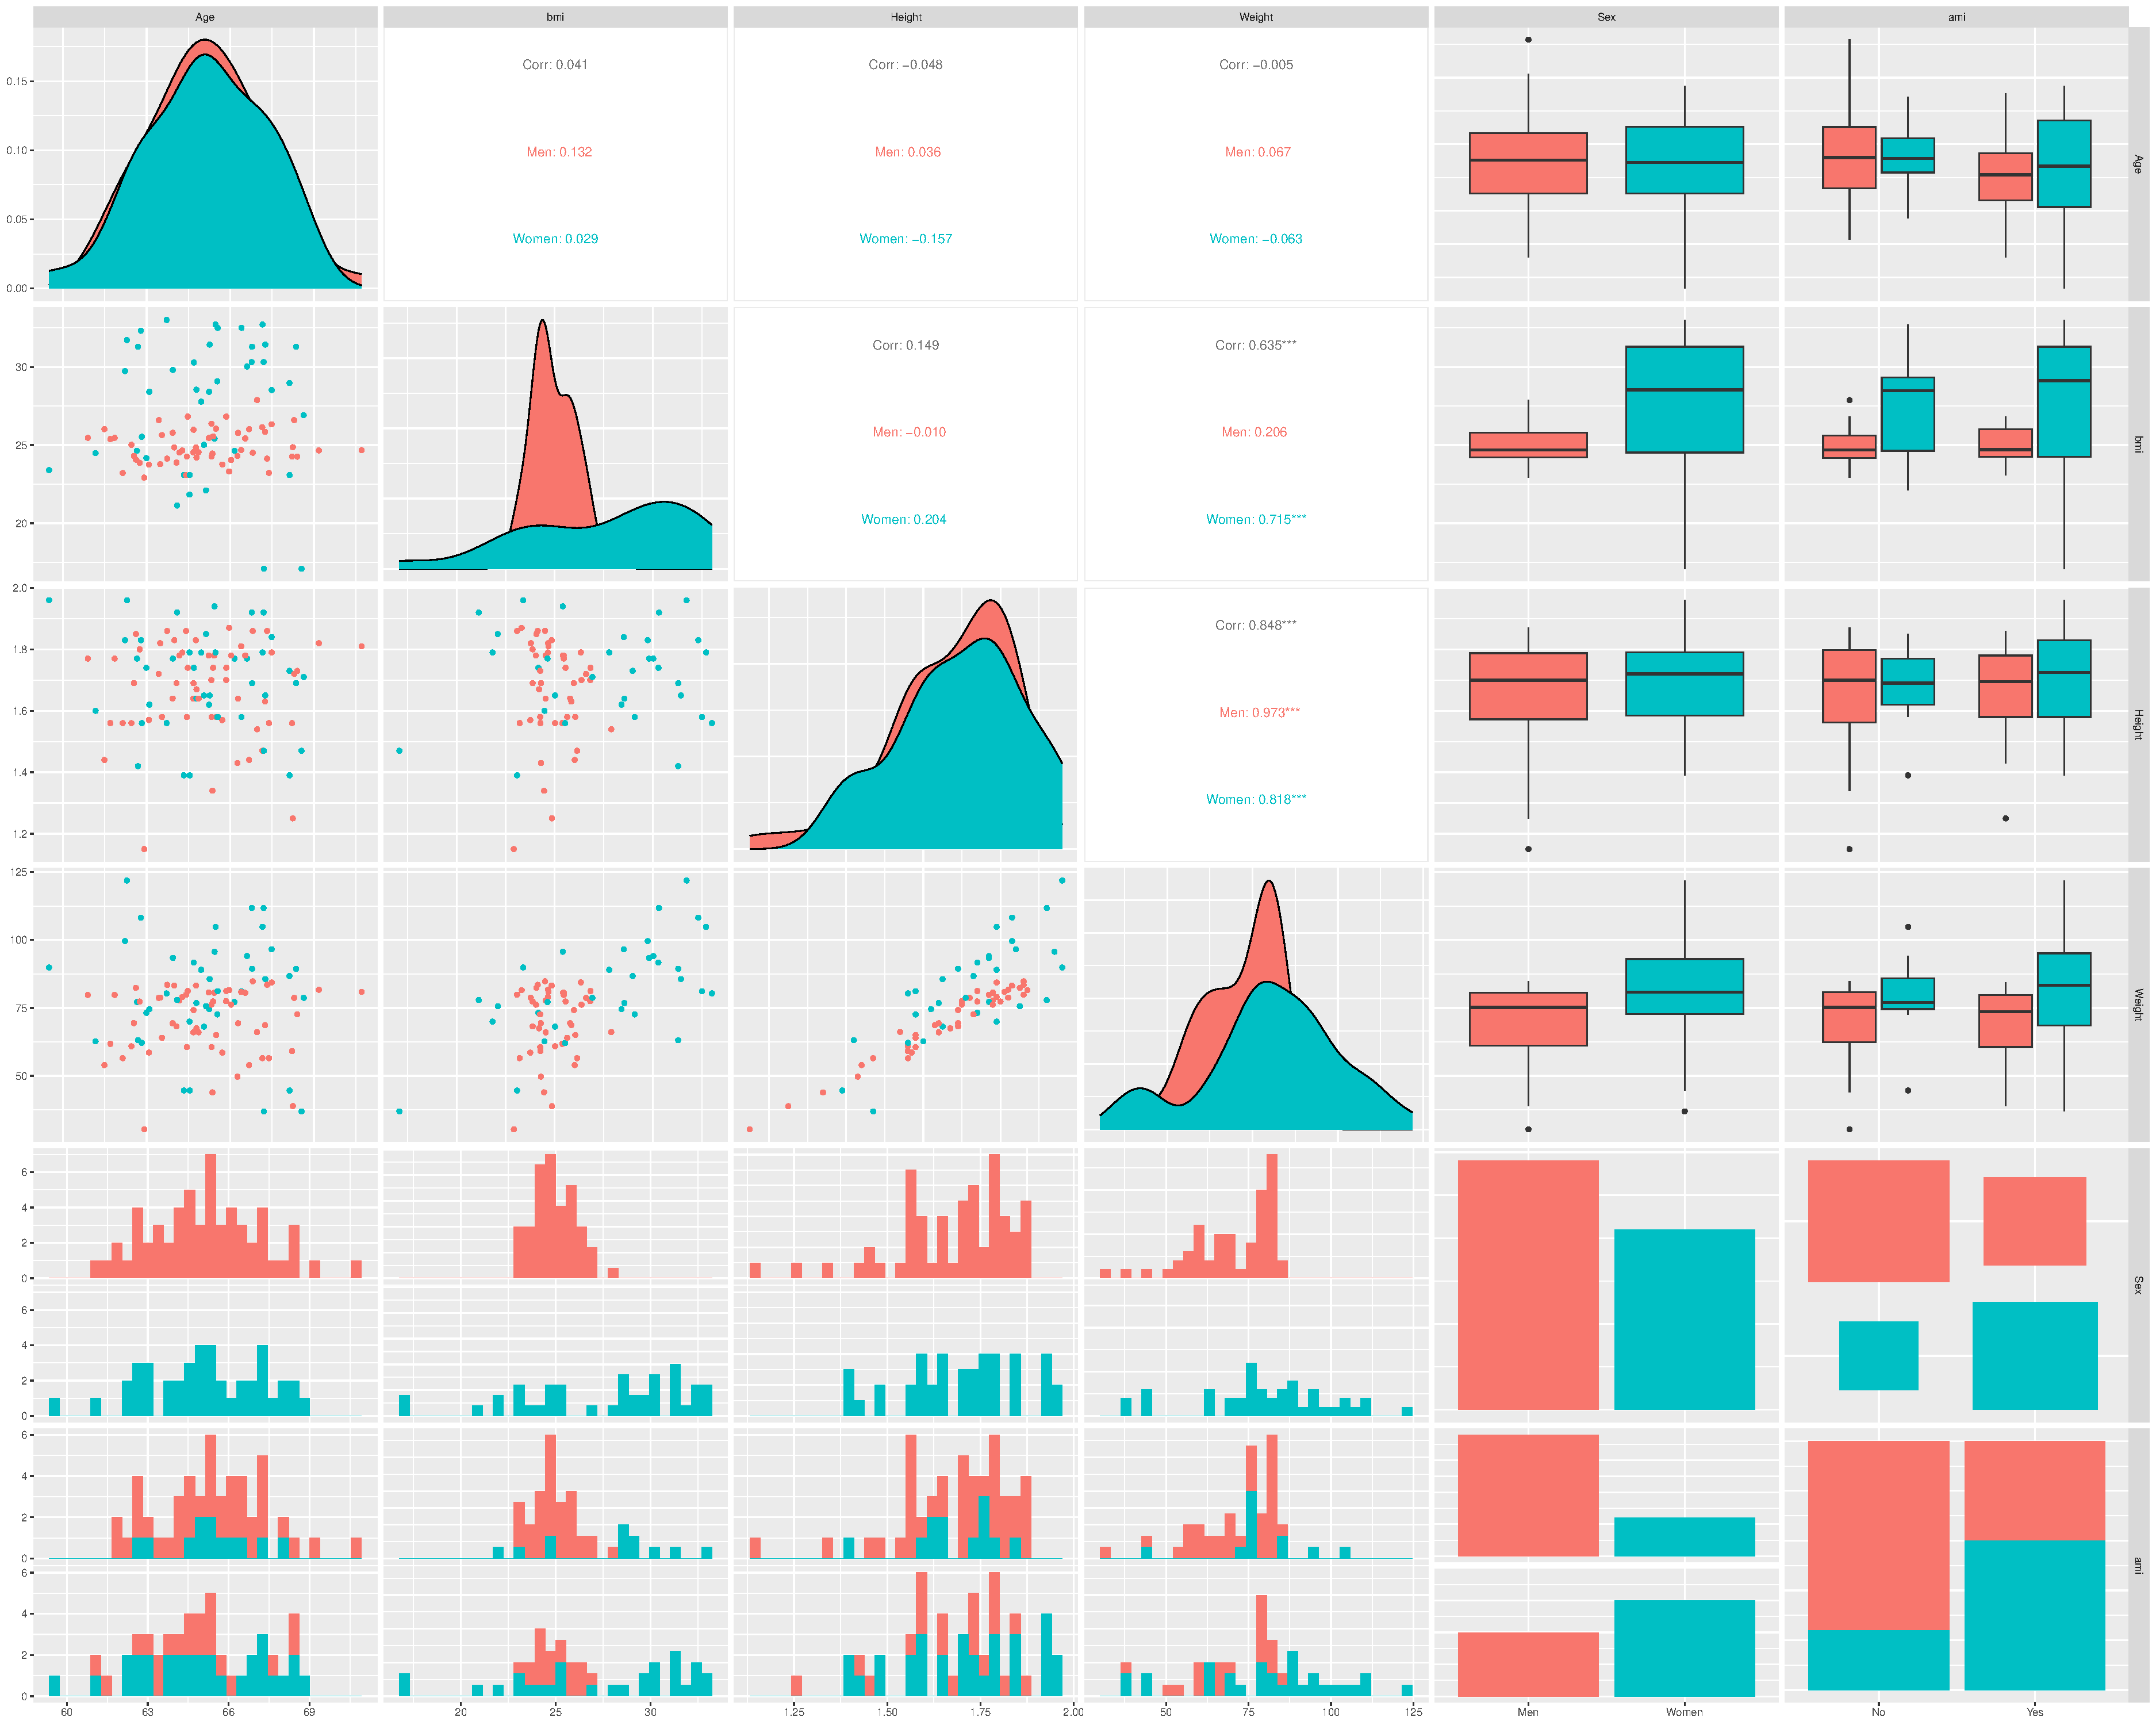
\includegraphics{./PR_4_lect_files/figure-pdf/unnamed-chunk-27-1.pdf}

\bookmarksetup{startatroot}

\hypertarget{references}{%
\chapter*{References}\label{references}}
\addcontentsline{toc}{chapter}{References}

\markboth{References}{References}

\hypertarget{refs}{}
\begin{CSLReferences}{1}{0}
\leavevmode\vadjust pre{\hypertarget{ref-bromanDataOrganizationSpreadsheets2018}{}}%
Broman, Karl W., and Kara H. Woo. 2018. {``Data Organization in
Spreadsheets.''} \emph{The American Statistician} 72 (1): 2--10.
\url{https://doi.org/10.1080/00031305.2017.1375989}.

\leavevmode\vadjust pre{\hypertarget{ref-gandrudReproducibleResearchRStudio2020}{}}%
Gandrud, Christopher. 2020. \emph{Reproducible Research with R and
RStudio}. Boca Raton, FL.

\leavevmode\vadjust pre{\hypertarget{ref-grolemundDataScience2017}{}}%
Grolemund, Garrett, and Hadley Wickham. 2017. \emph{R for Data Science}.
1st edition. Sebastopol, CA: O'Reilly Media.
\url{http://r4ds.had.co.nz/}.

\leavevmode\vadjust pre{\hypertarget{ref-kelionExcelWhyUsing2020}{}}%
Kelion, Leo. 2020. {``Excel: Why Using Microsoft's Tool Caused Covid-19
Results to Be Lost.''} \emph{BBC News}, October.
\url{https://www.bbc.com/news/technology-54423988}.

\leavevmode\vadjust pre{\hypertarget{ref-ruiz8020Data2017}{}}%
Ruiz, Armand. 2017. {``The 80/20 Data Science Dilemma.''}
\emph{InfoWorld}.
\url{https://www.infoworld.com/article/3228245/the-80-20-data-science-dilemma.html}.

\leavevmode\vadjust pre{\hypertarget{ref-thecarpentriesFormattingProblemsData}{}}%
The Carpentries. n.d. {``Formatting Problems \textendash{} Data
Organization in Spreadsheets for Ecologists.''} Accessed December 1,
2022.
\url{https://datacarpentry.org/spreadsheet-ecology-lesson/02-common-mistakes.html}.

\leavevmode\vadjust pre{\hypertarget{ref-wickhamTidyData2014}{}}%
Wickham, Hadley. 2014. {``Tidy Data.''} \emph{Journal of Statistical
Software} 59 (September): 1--23.
\url{https://doi.org/10.18637/jss.v059.i10}.

\end{CSLReferences}



\end{document}
